\ProvidesFile{thesis.tex}[2022-07-13 PurdueThesis thesis.tex file]

%
%  Be sure to sign up for the PurdueThesis mailing list at
%      https://engineering.purdue.edu/ECN/mailman/listinfo/purduethesis-list
%  so you learn of new versions of this software.  You must be on that
%  mailing list to receive help with this software.
%
%  This is the template root file for an example thesis (for master's
%  degree) or dissertation (for a PhD).  From now on "thesis" will
%  refer to both of these unless stated otherwise.
%
%  Search for "IMPORTANT" below to see three important comments.  One
%  concerns how to fix errors you get from using the "|" character.
%
%  LaTeX systems include auxiliary programs to do bibliographies,
%  indexes, etc.  The latexmk program runs the fewest programs needed
%  to update your thesis.  latexmk runs automatically on Overleaf.  If
%  you're LaTeXing your document on a non-Overleaf system you may need
%  to run latexmk manually.
%
%  To make a final PDF file before you turn in your thesis do
%      latexmk -g thesis
%  This makes sure than everything is done for your final version.
%
%  References cited below:
%
%  TM2017 is short for Thesis Manual 2017:
%    A Manual for the Preparation of Graduate Theses,
%    eighth revised edition,
%    Thesis and Dissertation Office,
%    Purdue University,
%    2017,
%    revised August 30, 2017,
%    http://www.purdue.edu/gradschool/documents/thesis/graduate-thesis-manual.pdf,
%    last retrieved on May, 8, 2021.
%
%  In this file, change the example information to your information.
%

% institution
% Choose an institution name from the following list:
%     VALUE                   COMMENT
%     Purdue University
%     Indiana University
%     University of Hawaii    don't include the 'okina character here,
%                             it will get printed automatically
%     University of Nevada    the real name is
%                                  University of Nevada, Reno
%                             but use this and use \ZZcampus below
%                             for consistency with other entries
\def\ZZinstitution{Purdue\space University}


% campus
% Choose a campus from the following list:
%     VALUE               COMMENT
%     Bloomington
%     Fort\space Wayne
%     Hammond
%     Indianapolis
%     Manoa               don't include the macron character here,
%                         it will get printed automatically
%     Reno
%     Westville
%     West\space Lafayette
\def\ZZcampus{West\space Lafayette}


% program
% Choose a program from the following list:
%     VALUE
%     Aeronautics and Astronautics
%     Agricultural and Biological Engineering
%     Agricultural Economics
%     Agronomy
%     American Studies
%     Animal Sciences
%     Anthropology
%     Art and Design
%     Aviation and Transportation Technology
%     Basic Medical Sciences
%     Biochemistry
%     Biological Sciences
%     Biology
%     Biomedical Engineering
%     Botany and Plant Pathology
%     Chemical Engineering
%     Chemistry
%     Chemistry and Chemical Biology
%     Child Development and Family Studies
%     Civil and Mechanical Engineering
%     Civil Engineering
%     Communication
%     Communications
%     Comparitive Pathobiology
%     Computer and Information Science
%     Computer and Information Technology
%     Computer Graphics Technology
%     Computer Science
%     Construction Management Technology
%     Consumer Science
%     Curriculum and Instruction
%     Earth, Atmospheric, and Planetary Sciences
%     Economics
%     Educational Studies
%     Electrical and Computer Engineering
%     Engineering Education
%     Engineering Technology
%     English
%     Entomology
%     Food Science
%     Forensic and Investigative Sciences
%     Forestry and Natural Resources
%     Health and Kinesiology
%     Health Sciences
%     History
%     History and Philosphy
%     Horticulture
%     Hospitality and Tourism Management
%     Human Development and Family Studies
%     Industrial and Physical Pharmacy
%     Industrial Engineering
%     Interdisciplinary Biomedical Studies Program
%     Interdisciplinary Studies (Comparitive Literature)
%     Languages and Cultures
%     Linguistics
%     Management
%     Materials Engineering
%     Mathematical Sciences
%     Mathematics
%     Mechanical and Energy Engineering
%     Mechanical Engineering
%     Mechanical and Civil Engineering
%     Medicinal Chemistry and Molecular Pharmacology
%     Nuclear Engineering
%     Nursing
%     Nutrition Science
%     Organizational Behavior and Human Resource Management
%     Pharmacy Practice
%     Philosophy
%     Philosophy and Literature
%     Physics
%     Physics and Astronomy
%     Political Science
%     Psychological Sciences
%     Public Health
%     Sociology
%     Speech, Language, and Hearing Sciences
%     Statistics
%     Technology Leadership and Innovation
%     Theatre
%     Veterinary Clinical Sciences
%     Youth Development and Agricultural Education
\def\ZZprogram{Electrical and Computer Engineering}

% degree
% Choose a degree from the following list:
%     Doctor of Audiology
%     Doctor of Nursing Practice
%     Doctor of Philosophy
%     Master of Arts
%     Master of Fine Arts
%     Master of Library Science
%     Master of Science
%     Master of Science in Agriculture
%     Master of Science in Aviation and Aerospace Management
%     Master of Science in Aeronautics and Astronautics
%     Master of Science in Agricultural and Biological Engineering
%     Master of Science in Building Construction Management
%     Master of Science in Biomedical Engineering
%     Master of Science in Chemical Engineering
%     Master of Science in Civil Engineering
%     Master of Science in Electrical and Computer Engineering
%     Master of Science in Engineering
%     Master of Science in Education
%     Master of Science in Human Resources Management
%     Master of Science in Industrial Engineering
%     Master of Science in Industrial Technology
%     Master of Science in Mechanical Engineering
%     Master of Science in Materials Engineering
%     Master of Science in Nuclear Engineering
\def\ZZdegree{Doctor of Philosophy}

% author
% Put your name here.
\def\ZZauthor{Mark Senn}

% document
% Choose a document from the following list:
%     A Directed Research Project
%     A Dissertation
%     A Master's Bypass Report
%     A Preliminary Report
%     A Thesis
\def\ZZdocument{A Thesis}

% graduation
% Chose a month from
%     May
%     August
%     December
% followed by a space
% then choose a year from 2020 to 2030.
\def\ZZgraduation{August 2022}

% title
% If you need to manually split the title,
% over several lines do, for example,
% \def\ZZtitle{%
%   % The "[-5pt]" is to correct a problem with vertical spacing.
%   This is the first line of the Title\\[-5pt]
%   This is the second line of the Title\\
%   This is the third line of the Title%
% }
\def\ZZtitle{THIS IS THE THESIS TITLE}


% showcolophon
% Print the ap-colophon.tex file at the end of the document?
% THE SUBMITTED COPY OF YOUR THESIS MUST BE RUN WITH ZZshowcolophon = {false}.
\def\ZZshowcolophon{false}

% showdiagonalline
% Show a diagonal line from lower left to center
% of main printed part of page?
% THE SUBMITTED COPY OF YOUR THESIS MUST BE RUN WITH ZZshowdiagonalline = {false}.
\def\ZZshowdiagonalline{false}

% showgridlines
% Show grid lines on main printed part of page?
% Vertical and horizontal grid lines are put
% in the normal printed part of the page---this
% includes lines where the margins are.
% THE SUBMITTED COPY OF YOUR THESIS MUST BE RUN WITH ZZshowgridlines = {false}.
\def\ZZshowgridlines{false}

% showmarginlines
% Show margin lines on the edge of the normal printed part of the page?
% Margin lines show where the margins are.
% THE SUBMITTED COPY OF YOUR THESIS MUST BE RUN WITH ZZshowmarginlines = {false}.
%     VALUE    MEANING
%     false    don't show marginlines
%     true     show marginlines
\def\ZZshowmarginlines{false}

% showtimestamp
% Show, for example, a "compiled on  Tuesday  2021-03-02  17:16:24-04"
% timestamp in the upper right corner of page?
%     VALUE    MEANING
%     false    don't show timestamp
%     true     show timestamp
% THE SUBMITTED COPY OF YOUR THESIS MUST BE RUN WITH ZZshowtimestamp = {false}.
\def\ZZshowtimestamp{false}

% todonotes
% Set things up for todonotes.
%     VALUE    MEANING
%     false    don't put todo notes in PDF file
%     true     put 0.8 inch wide todo notes in PDF file
%     wide     put 3.8 inch wide todo notes in PDF file, do not send
%              todonotes = wide output to a printer
% THE SUBMITTED COPY OF YOUR THESIS MUST BE RUN WITH todonotes = {false}.
\def\ZZtodonotes{false}

% Mark Senn uses an `optional-debugging-code.tex file' but does not
% distribute it.  The following line won't do anything if you don't
% have an optional-debugging-code.tex file so you can leave it the
% way it is.
\InputIfFileExists{optional-debugging-code.tex}{}{}

% The \includeonly command can be used to only include some
% files that have \include commands below.  This is handy
% to only include some files so your document will LaTeX
% faster or if you're trying to narrow down where an error
% occurs.  You can use
%     \includeonly{ch-introduction}
% to only include ch-introduction.tex, or
%     \includeonly{ch-introduction,ap-about-appendices}
% to include ch-introduction.tex and ap-about-appendices.tex.
% More files can be added---just put ',' between the names.
% Comment out the following line before submitting the
% final copy of your thesis.
% \includeonly{...}


\documentclass{PurdueThesis}

\def\ZZatinformation{}
% If you are at the Hammond or Westville campus
% remove the "%" from the begining of the next line.
%\def\ZZatinformation{~at~Purdue~Northwest}

% PurdueThesis.cls loads the rotating package which loads the graphicx
% package.  From page 12 of "Packages in the `graphics' bundle", 2021-03-05,
% retrieved 2021-06-16, at https://texdoc.org/serve/grfguide.pdf/0
%     \graphicspath{<dir-list>}
%
%         This optional declaration may be used to specify a list of
%         directories in which to search for graphics files.  The
%         format is the same as for the LaTeX 2e primitive \input@path.
%         A list of directories, each in a {} group (even if there is
%         only one in the list).  For example:
%             \graphicspath{{eps/}{tiff/}}
%         would cause the system to look in the subdirectories eps and
%         tiff of the current directory.  (All modern TeX systems use /
%         as the directory separator, even on Windows.)
%
%         The default setting of this path is \input@path that is:
%         graphics files will be found whereever TeX files are found.
%
% Look in the "graphics" subfolder for graphics files.
% This is done to reduce the number of files in the main thesis folder
% so the ones in there are easier to find.
\graphicspath{{graphics/}}

% Look in the "packages" subfolder for packages.
% This is done to reduce the number of files in the main thesis folder
% so the ones in there are easier to find.
\makeatletter
  \def\input@path{{packages/}}
\makeatother

%
% Configure bibliography.
%
% To override the default choices picked by \ConfigureBibliography, change,
% for example,
%     \ConfigureBibliography
% to
%     % \ConfigureBibliography
%     \usepackage[backend=biber, citestyle=apa, dashed=false, sortcites=true, style=apa]{biblatex}
%     \addbibresource{all-biblatex.bib}
%     See
%         https://tex.stackexchange.com/questions/134191/line-breaks-of-long-urls-in-biblatex-bibliography
%     \setcounter{biburllcpenalty}{7000}
%     \setcounter{biburlucpenalty}{8000}
% Detailed information for what ConfigreBibliography
% does is in PurdueThesis.cls.
\ConfigureBibliography

% If you don't want to ignore urldate fields,
% comment out (put "%" before) the next ten lines.
\DeclareSourcemap
  {
    \maps[datatype=bibtex]
      {
        % Ignore "urldate = {...}" in .bib files.
        % See the first complete example on page 201 of
        %     https://mirrors.rit.edu/CTAN/macros/latex/contrib/biblatex/doc/biblatex.pdf
        \map { \step[fieldset=urldate, null] }
      }
  }

% To let {\bfseries\scshape text} work as expected.
% See
%     https://tex.stackexchange.com/questions/27411/small-caps-and-bold-face
\usepackage{bold-extra}

% For chemical figures.
\usepackage{chemfig}

% For typesetting cryptography pseudocode, algorithms, and protocols.
% See
%     https://mirror.las.iastate.edu/tex-archive/macros/latex/contrib/cryptocode/cryptocode.pdf
\usepackage
[
  n,            % or lambda
  advantage,
  operators,
  sets,
  adversary,
  landau,
  probability,
  notions,
  logic,
  ff,
  mm,
  primitives,
  events,
  complexity,
  oracles,
  asymptotics,
  keys,
]
{cryptocode}

% IMPORTANT
% Define
%    \VerbatimInput[options]{filename}
%    \begin{VerbatimOut}{filename} ... \end{VerbatimOut}.
\usepackage{fancyvrb}
  % Define a special character as an abbreviation to enclose verbatim
  % text.  For example, the next line allows one to type "|word|"
  % instead of, for example, "\verb+word+".  PROBLEM: USING | IN
  % MATHEMATICS WITH "\DefineShortVerb{\|}" WILL CAUSE AN ERROR.  If you
  % want to use a "|" in math mode comment out the
  % "\DefineShortVerb{\|}" and see these about how to get the correct
  % horizontal spacing:
  %     https://tex.stackexchange.com/questions/52901/why-is-mid-so-called
  %     https://ctan.math.washington.edu/tex-archive/macros/latex/contrib/braket/braket.pdf
  \DefineShortVerb{\|}

% For \InpuutIfFileExists.
\usepackage{filehook}

% So "_" will work in URLs when using BibTeX.
\usepackage[T1]{fontenc}

% For testing.
\usepackage{listings}

% For chemical equations.
% See
%     https://ctan.org/pkg/mhchem?lang=en
% From the "Package documentation" linked-to document
%     mhchem needs a couple of other packages.
%     For instance, expl3, amsmath and calc.
\usepackage[version=4]{mhchem}
  % If I'm loading the package to just define a few new commands I'll indent
  % two spaces right after loading the package and define the few new
  % commands here.  If I'm defining more than a few commands I usually do it
  % after loading all the packages.
  % Define "\nitrate" to be the chemical symbol for nitrate.
  \newcommand{\nitrate}{\ce{NO3{-}}}
  % Define "\pnitrate" (short for "parenthesized nitrate") to be the chemical
  % symbol for nitrate surrounded by parentheses.
  \newcommand{\pnitrate}{(\nitrate)}
  % "Define \vpnitrate" (short for "verbose parenthesized nitrate") to be
  % the word "nitrate" followed by a space followed by the chemical symbol
  % for nitrate with parentheses around it.
  \newcommand{\vpnitrate}{nitrate (\nitrate)}

% For
%     \cancel
%     \highlight
% See
%     http://mirrors.ctan.org/macros/latex/contrib/siunitx/siunitx.pdf
% pages 11--12.
 \usepackage{cancel}


% Redefine description, enumerate, and itemize lists.
% See
%     https://mirrors.concertpass.com/tex-archive/macros/latex/contrib/enumitem/enumitem.pdf
% \usepackage{enumitem}
% \setlist[itemize]{leftmargin=7pt,rightmargin=24pt}



% This gets rid of
%     [5] (./thesis.toc
%     ! Undefined control sequence.
%     \vbox_set:Nn ...box:D {\color_group_begin: #2\par
%                                                       \color_group_end: }
%     l.32 ...}Basic Circuit Components}{31}{section.67}
%                                                       %
%     ?
% and
%     [6]
%     ! Undefined control sequence.
%     \vbox_set:Nn ...box:D {\color_group_begin: #2\par
%                                                       \color_group_end: }
%     l.61 ...rline {P.1}Frenchspacing}{67}{section.445}
%                                                       %
%     ?
% errors.
% See
%     https://github.com/latex3/latex2e/issues/73
\usepackage{etoc}

% Define \setmaxprintline{number_of_columns}.
% \usepackage{hardwrap}

% For indexing.  Making an index is optional.
% Make these commands available:
%     COMMAND           DESCRIPTION
%     \index{string}    put "string" in index information
%     \makeindex        save information to make the index
%     \printindex       print the index
% See
%     https://ctan.org/pkg/makeidx?lang=en
% for more information.
\usepackage{makeidx}
  % By default \index ignores its argument.
  % This activates indexing.
  \makeindex
  % The "chapter name" for the index.
  \renewcommand{\indexname}{INDEX}

% The mathtools package
% (see http://mirror.utexas.edu/ctan/macros/latex/required/amsmath/amsmath.pdf)
% loads the amsmath package which defines the
%     align
%     align*
%     alignat
%     alignat*
%     equation
%     equation*
%     flalign
%     flalign*
%     gather
%     gather*
%     multitaper
%     multitaper*
%     split
% environments and extends amsmath by defining many other commands.
% See
%     https://ctan.org/pkg/amsmath
% for information about amsmath and
%     http://ctan.math.washington.edu/tex-archive/macros/latex/contrib/mathtools/mathtools.pdf
% for information about mathtools.
\usepackage{mathtools}

% Define \includemedia.
\usepackage{media9}

% Define \begin{multicols}{number_of_columns} ... \end{multicolumns}.
% Used in ap-text.tex.
\usepackage{multicol}

% Define \ditto.
\usepackage{pa-ditto}

% Define \FigureDash.
% \FigureDash is a dash the width of a digit in the current font.
\usepackage{pa-figure-dash}

% For PurdueThesis, PuTh, TeX, LaTeX, etc. related logos.
\usepackage{pa-logos}

% The ISO 80000-2:2019 standard recommends the following.
% The pa-mismath package is loaded to provide these features.
%
% The "d" in, for example, "dx" mathematical integrals should use a
% roman "d".  "\di x" expands to "\,mathrm{d}\/x" to do this
% automatically.
%
% Put e, i, j, and pi in an upright font to indicate they are
% constants.  I had thesis.tex set up to do this automatically and got
% complaints that i was not in a math italic font.  By default I'm now
% setting things up so e and pi are set in an upright font
% automatically and i and j are set in a math italic font.
% IN MATH MODE
%     INPUT   OUTPUT                      INPUT   OUTPUT
%     e       upright e (constant)        \ite    math italic e (variable)
%     i       math italic i (variable)    \i      upright i (constant)
%     j       math italic j (variable)    \j      upright j (constant
%     \pi     upright pi (constant)       \itpi   math italic pi (variable)
\usepackage{pa-mismath}
  \enumber
  \pinumber
  \newcommand{\ite}{\mit{e}}

% Define \MyRepeat{what}{repeat}.
% Repeat "what" "repeat" number of times.
\usepackage{pa-repeat}

% Define \FloatBarrier.
% \FloatBarrier process all unproccesed floats (tables, figures, etc.).
\usepackage{placeins}

% Define \hl.
% Undefine \st so soul will load without an error.
% I hope \st wasn't used for something important!
\let\st\relax
\usepackage{soul}

% Define \textcent.
\usepackage{textcomp}

% !!! This doesn't work yet, figure it out later.
% For \textprimstress.
% \usepackage{tipa}

% Needed for chapter "Graphics", section "TikZ and PGF".
\usepackage{tikz}
  % Needed to customize arrows.
  \usetikzlibrary{arrows.meta}
  % For electrical diagrams.
  % Uses the TikZ package.
  % The circuitikz name is short for "circuit TikZ".
  \usepackage{circuitikz}
  %
  \usepackage{menukeys}
  %
  % Needed for 3D TikZ stuff.
  \usetikzlibrary{3d}
  %
  % Needed for pa-typographic-conventions package.
  \usetikzlibrary{calc,shadows,shapes.misc,shapes.symbols}
  %
  % Needed for putting text along a path.
  \usetikzlibrary{decorations.text}
  %
  % Draw TikZ decorations.
  % Needed for at least the Kalman filter system model graphic.
  \usetikzlibrary{decorations.pathmorphing} % noisy shapes
  %
  % Fit shapes to coordinates.
  % Needed for at least the Kalman filter system model graphic.
  \usetikzlibrary{fit}
  %
  % Draw the background after the foreground.
  \usetikzlibrary{backgrounds}	% drawing the background after the foreground

% IMPORTANT
% Needed for the Feynman diagram in ap-physics.tex.
% Tikz-feynman requires LuaLaTeX instead of pdflatex be run.
\usepackage[compat=1.1.0]{tikz-feynman}

% The vertical space between a table heading and the table contents
% in a tabular environment.
\newcommand{\tabularspace}{\noalign{\vspace*{2pt}}}

% For \sfrac, used to do slanted fractions, similar to, e.g., 1/2,
% but 1 is small and high and 2 is small and low.
\usepackage{xfrac}


% Define \I.
% \I1 does \indent once, \I2 does \indent twice, etc.
\newcommand{\I}[1]{\MyRepeat{\indent}{#1}}

% Define \MyI.
% Typeset my input.
\long\def\MyI#1%
  {%
    {%
      \fontsize{8}{10}\tt
      \VerbatimInput
        [
          firstnumber = 1,
          numbers     = left,
          xleftmargin = 0.33in,
        ]%
        {#1}
    }%
  }

% Define \MyIO.
% Typeset my input and output.
% The input will all be on the same page.
% The output may be split over multiple pages.
\newcommand{\MyIO}
  {%
    \input{z.out}

    {%
      \ZZbaselinestretch{1}
      \fontsize{8}{9.6}\tt
      \VerbatimInput
        [
          firstnumber = 1,
          numbers     = left,
          xleftmargin = 0.33in,
        ]
        {z.out}
    }
    \FloatBarrier
  }

% Define \MyIOS.
% Typeset my input and output.
% The input may be split over multiple pages.
% The output may be split over multiple pages.
% This doesn't work right:
%     o  Putting a \vbox around the input and output
%        does not allow todoindex entries to be listed.
%     o  Using \vfilneg at beginning and end of definition
%        screws up vertical spacing.
% \newcommand{\MyIOS}
% {%
%   \input{z.out}
%
%   {%
%     \fontsize{8}{10}\tt
%     \VerbatimInput
%     [
%       firstnumber = 1,
%       numbers     = left,
%       xleftmargin = 0.33in,
%     ]{z.out}%
%   }
% }

% Define \MyIOT.
% Typset my input and output together on the same page.
% This doesn't work right:
%     o  Putting a \vbox around the input and output
%        does not allow todoindex entries to be listed.
%     o  Using \vfilneg at beginning and end of definition
%        screws up vertical spacing.
% \def\MyIOT
% {%
%   \vfilneg
%   % \vbox
%   {%
%     \input{z.out}%
%     \fontsize{8}{10}\tt
%     \VerbatimInput[
%       firstnumber = 1,
%       numbers     = left,
%       xleftmargin = 0.33in,
%     ]{z.out}%
%   }%
%   \FloatBarrier
%   \vfilneg
% }

% Define \NL (newline) so LaTeX goes to the next output line.
% Just doing \\ complains
%     ! LaTeX Error: There's no line here to end.
% \mbox{} is an empty math box.
\newcommand{\NL}{\mbox{}\\}

% In this document I use in-line tables a lot.
% These are tables that are put in the document
% where I want them to appear and they don't
% use \begin{table} ... \end{table}

\newenvironment{inlinetable}
  {%
    \begingroup
      \singlespace
      \mbox{}\\[-9pt]%
      \noindent
      \hspace*{2\parindent}%
      \ignorespaces
  }
  {%
      \mbox{}\\
    \endgroup
  }

% Print a list of files used and their version numbers in the log file.
\listfiles


% \def\bibindent{0em}
% Customize the bibliography.
% \DefineBibliographyStrings{english}{
%   urlfrom = {URLFROM},
%   urlseen = {URLSEEN}
% }

% For typographical conventions stuff including
%     \Emph{...}
%     \First{...}
%     \Keys{...}
%     \Literal{...}
%     \Menu{...}
%     \Place{...}
%     \Shell{...}
% This must be after
%     \usepackage{tikz}
\usepackage{pa-typographic-conventions}

% For the \begin{example} ... \end{example} environment
% used in ap-linguistics.tex.
\usepackage{covington}
\usepackage{slgloss}

% "CTAN---Comprehensive" did not get hyphenated and extended
% into the right margin when using BibLaTeX and the apa style.
% These did not change it:
%     \hyphenation{Com-pre-hen-sive}
%     \hyphenation{CTAN---Com-pre-hen-sive}
% I changed    publisher = {CTAN---Comprehensive TeX Archive Network},
% to           publisher = {CTAN---Com\-pre\-hen\-sive TeX Archive Network},
% in my all-biblatex.bib file and it worked as expeceted.
% If you need to change the hyphenation points of a word in the text
% you can do, for example,
%     \hyphenation{ve-ry-od-dly-hy-phen-at-ed}


\begin{document}

% Set the table of contents depth.
% USE    TO HAVE THE FOLLOWING in THE TABLE OF CONTENTS.
% 0      chapters
% 1      the above plus sections
% 2      the above plus subsections
% 3      the abeve plus subsubsections
\setcounter{tocdepth}{3}

\maketitle

% Define front matter
%     dedication
%     acknowledgments
%     preface
%     table of contents
%     list of tables
%     list of figures
%     list of symbols
%     abbreviations
%     nomenclature
%     glossary
%     abstract
\ProvidesFile{ch-front.tex}[2022-07-13 front matter chapter]
%
%  This is ``front matter'' for the thesis.
%
%  REFERENCES
%
%    TCMOS17
%      The Chicago Manual of Style Online, 17th edition.
%      https://www.chicagomanualofstyle.org/home.html
%      retrieved on 2020-02-29
%
%    TEMPL
%      Thesis and Disertation Office Templates.
%      https://www.purdue.edu/gradschool/research/thesis/templates.html
%      retrieved on 2020-02-29
%
%    WNNCD
%    Webster's Ninth New Collegiate Dictionary.
%

%
%   Only Purdue University uses this page
%
%   Comment out \begin{statement} through \end{statement}
%   if you are not at Purdue University.
%
% Statement of Thesis/Dissertation Approval Page
% This page is REQUIRED.  The page should be numbered "2"
% and should NOT be listed in your TABLE OF CONTENTS.
\begin{statement}
  % Delete or add \entry commands as needed for all committe members.
  \entry{Dr.~John Doe, Chair}{School of Aeronautics and Astronautics}
  \entry{Dr.~Jane Doe}{School of Aeronautics and Astronautics}
  \entry{Dr.~Jim Doe}{School of Aeronautics and Astronautics}
  % There should be one \approvedby command containing the
  % "FORM 9 THESIS FORM HEAD NAME HERE" (from TEMPL, retrieved on 2020-03-01).
  \approvedby{Dr.~Buck Doe}
\end{statement}

% Dedication page is optional.
% A name and often a message in tribute to a person or cause.
% References: WEB9 332.
\begin{dedication}
  To graduate students
\end{dedication}

% Acknowledgements page is optional but most theses include
% a brief statement of appreciation or recognition of special
% assistance.
\begin{acknowledgments}
  Purdue University's Engineering Computer Network
  and Graduate School helped fund \PurdueThesisLogo\ development.
\end{acknowledgments}

% The preface is optional.
% References: TCMOS17 1.49, WEB9 927.
\begin{preface}
  This is the preface.
\end{preface}

% The Table of Contents is required.
% The Table of Contents will be automatically created for you
% using information you supply in
%     \chapter
%     \section
%     \subsection
%     \subsubsection
%     commands.
\pdfbookmark{TABLE OF CONTENTS}{Contents}
\tableofcontents

% If your thesis has tables, a list of tables is required.
% The List of Tables will be automatically created for you using
% information you supply in
%     \begin{table} ... \end{table}
% environments.
\listoftables

% If your thesis has figures, a list of figures is required.
% The List of Figures will be automatically created for you using
% information you supply in
%     \begin{figure} ... \end{figure}
% environments.
\listoffigures

% If your thesis has listings, a list of listings is required.
% The List of Listings will be automatically created for you using
% information you supply in
%     \begin{ZZlisting} ... \end{ZZlisting}
% environments.
\ZZlistoflistings

% If your thesis has protocols, you may want to do a list of protocols.
% The List of Protocols will be automatically created for you using
% information you supply in
%     \begin{protocol} ... \end{protocol}
% environments.
\listofprotocols

% If your thesis has schemes, you may want to do a list of schemes.
% The List of Schemes will be automatically created for you using
% information you supply in
%     \begin{scheme} ... \end{scheme}
% environments.
\listofschemes

% List of Symbols is optional.
\begin{symbols}
  \(m\)& mass\cr
  \(v\)& velocity\cr
\end{symbols}

% List of Abbreviations is optional.
\begin{abbreviations}
  abbr& abbreviation\cr
  bcf& billion cubic feet\cr
  BMOC& big man on campus\cr
\end{abbreviations}

% Nomenclature is optional.
\begin{nomenclature}
  alanine& 2-Aminopropanoic acid\\
  gasoline& a transparent,
    petroleum-derived flammable liquid that is used primarily
    as a fuel in most spark-ignited internal combustion engines
    \cite{wikipedia-gasoline}\\
  valine& 2-Amino-3-methylbutanoic acid\\
  Valvoline& Valvoline Inc.~is an American manufacturer
    and distributor of Valvoline-brand automotive oil,
    additives,
    and lubricants.
    It also owns the Valvoline Instant Oil Change
    and Valvoline Express Care chains of car repair centers.
    As of 2016,
    it is the second largest oil change service provider in the United States
    with 10\% market share
    and 1,050 locations.
    \cite{wikipedia-valvoline}\\
  \mbox{}\\
  \rlap{you can divide these into categories if you want}\\
  \mbox{}\\
  \rlap{\bfseries Biology}\\
  alanine& 2-Aminopropanoic acid\\
  valine& 2-Amino-3-methylbutanoic acid\\
  \rlap{\bfseries Transportation}\\
  gasoline& a transparent,
    petroleum-derived flammable liquid that is used primarily
    as a fuel in most spark-ignited internal combustion engines
    \cite{wikipedia-gasoline}\\
  Valvoline& Valvoline Inc.~is an American manufacturer
    and distributor of Valvoline-brand automotive oil,
    additives,
    and lubricants.
    It also owns the Valvoline Instant Oil Change
    and Valvoline Express Care chains of car repair centers.
    As of 2016,
    it is the second largest oil change service provider in the United States
    with 10\% market share
    and 1,050 locations.
    \cite{wikipedia-valvoline}
\end{nomenclature}

% Glossary is optional.
\begin{glossary}
  philtrum& the groove between the nose and upper lip\\
  septem& the cartilage in the nose that separates the nostrils\\
  supercalifragilisticexpialidocious&
    a nonsense word,
    originally used esp.~by children,
    and typically expressing excited approbation:
    fantastic,
    fabulous
    \cite{oed-super...}\\
  test entry&
    This is a a long test sentence.
    This is a a long test sentence.
    This is a a long test sentence.
    This is a a long test sentence.
    This is a a long test sentence.
    This is a a long test sentence.
    This is a a long test sentence.
    This is a a long test sentence.
    This is a a long test sentence.
    This is a a long test sentence.\\
  test entry&
    This is a a long test sentence.
    This is a a long test sentence.
    This is a a long test sentence.
    This is a a long test sentence.
    This is a a long test sentence.
    This is a a long test sentence.
    This is a a long test sentence.
    This is a a long test sentence.
    This is a a long test sentence.
    This is a a long test sentence.
    This is a a long test sentence.
    This is a a long test sentence.
    This is a a long test sentence.
    This is a a long test sentence.
    This is a a long test sentence.
    This is a a long test sentence.
    This is a a long test sentence.
    This is a a long test sentence.
    This is a a long test sentence.
    This is a a long test sentence.
    This is a a long test sentence.
    This is a a long test sentence.
    This is a a long test sentence.
    This is a a long test sentence.
    This is a a long test sentence.
    This is a a long test sentence.
    This is a a long test sentence.
    This is a a long test sentence.
    This is a a long test sentence.
    This is a a long test sentence.
    This is a a long test sentence.
    This is a a long test sentence.
    This is a a long test sentence.
    This is a a long test sentence.
    This is a a long test sentence.
    This is a a long test sentence.
    This is a a long test sentence.
    This is a a long test sentence.
    This is a a long test sentence.
    This is a a long test sentence.\\
\end{glossary}

% Abstract is required.
% Reference: PU 17.
\begin{abstract}%
  \PurdueThesisLogo\ is a \LaTeX\ document class used for
  master's bypass reports,
  master's theses,
  PhD dissertations,
  and PhD preliminary reports.
  This template demonstrates how to use \PurdueThesisLogo.

\end{abstract}


%
% Put chapter \include commands here.
%

% Introductions may precede the first chapters or major divisions of theses.
% Reference: TM2017, page 31.
\ProvidesFile{ch-introduction.tex}[2022-07-10 introduction chapter]

\chapter{INTRODUCTION}

{\sl\TeXLogo\/} is a typesetting system for the creation of beautiful books---%
and especially for books that contain lots of mathematics
\cite[page v]{knuth2012}.

{\sl\LaTeXLogo\/} is a software system for typesetting documents
\cite[back cover]{lamport1994}.
It extends \TeX\ with more natural chapter,
section,
etc.~commands that are easier to use.
\LaTeX\ has document classes for
articles,
books,
reports,
etc.

{\sl\LuaLaTeXLogo\/} adds
the Lua scripting language,
\MetaPostLogo
\cite{metapost-on-the-web},
OpenType font capability,
and UTF-8
\cite{wikipedia-utf-8}
text encoding for Unicode
\cite{wikipedia-unicode}
to \LaTeXLogo.

{\sl\PurdueThesisLogo\/}
({\sl\PuThLogo} for short---rhymes with tooth)
is a \LaTeX\ document class used for Purdue theses,
dissertations,
master’s bypass reports,
and PhD preliminary reports.
This template demonstrates how to use PurdueThesis.
PurdueThesis is intended to support all Purdue campuses,
programs,
and graduate degrees.

Figure \ref{fi:lualatex-system-flowchart} shows a simplified \LuaLaTeXLogo\ System Flowchart.
Overleaf
\cite{overleaf}
uses latexmk
\cite{latexmk}
to run
|biblatex| or |bibtex|,
|makeindex|,
and |pdflatex| automatically
so the minimum amount of work is done.
On Linux,
MacOS,
and Windows you can run the programs individually
or use |latexmk|---I recommend using |latexmk|.
  
\begin{figure}
  \centering
  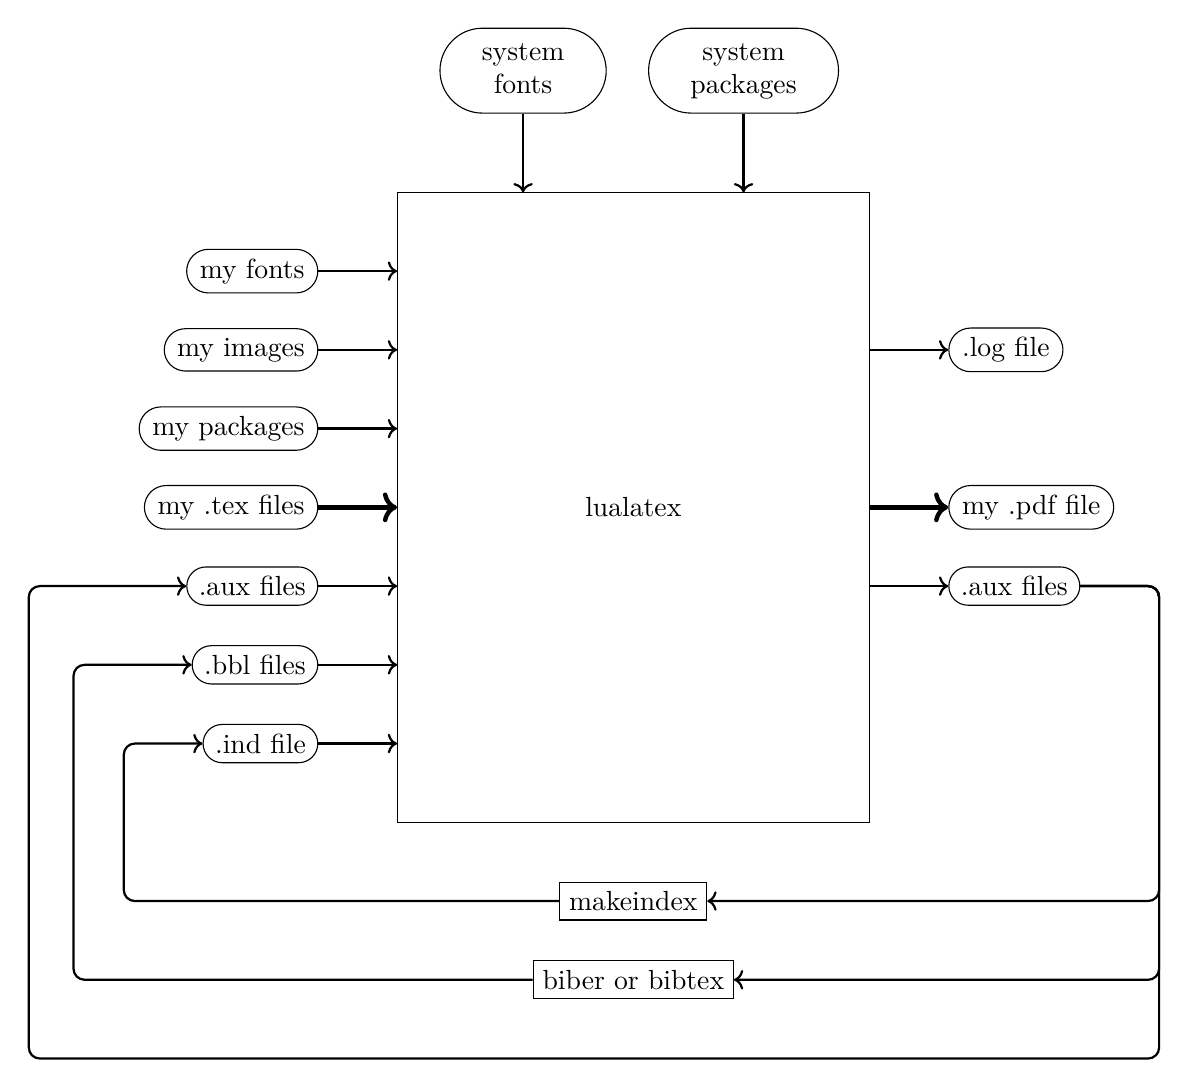
\begin{tikzpicture}{scale=0.9}

    \tikzset{font={\fontsize{10pt}{12pt}\selectfont}}

    % Large rectangle.
    \coordinate (pdflatex-nw-c) at (0,8);  \coordinate (pdflatex-ne-c) at (6,8);
    \coordinate (pdflatex-sw-c) at (0,0);  \coordinate (pdflatex-se-c) at (6,0);

    % Draw large rectangle.
    \draw (pdflatex-sw-c) -- (pdflatex-nw-c) -- (pdflatex-ne-c) -- (pdflatex-se-c) -- cycle;

    % West edge of rectangle.
    \coordinate (my-fonts-c)       at (0,7);  \coordinate (my-fonts-w-c)     at ($(my-fonts-c)     + (-1,0)$);
    \coordinate (my-images-c)      at (0,6);  \coordinate (my-images-w-c)    at ($(my-images-c)    + (-1,0)$);
    \coordinate (my-packages-c)    at (0,5);  \coordinate (my-packages-w-c)  at ($(my-packages-c)  + (-1,0)$);
    \coordinate (my-tex-files-c)   at (0,4);  \coordinate (my-tex-files-w-c) at ($(my-tex-files-c) + (-1,0)$);
    \coordinate (w-aux-files-c)    at (0,3);  \coordinate (w-aux-files-w-c)  at ($(w-aux-files-c)  + (-1,0)$);
      \coordinate (w-aux-files-w-w-c)         at ($(w-aux-files-w-c) + (-1,0)$);
    \coordinate (bbl-files-c)      at (0,2);  \coordinate (bbl-files-w-c)    at ($(bbl-files-c)    + (-1,0)$);
    \coordinate (ind-file-c)       at (0,1);  \coordinate (ind-file-w-c)     at ($(ind-file-c)     + (-1,0)$);

    % North edge of rectangle.
    \coordinate (system-fonts-c)    at (1.6,8);  \coordinate (system-fonts-n-c)    at ($(system-fonts-c)    + (0,1)$);
    \coordinate (system-packages-c) at (4.4,8);  \coordinate (system-packages-n-c) at ($(system-packages-c) + (0,1)$);

    % East edge of rectangle.
    \coordinate (log-file-c)      at (6,6);  \coordinate (log-file-e-c)      at ($(log-file-c) + (1,0)$);
    \coordinate (my-pdf-file-c)   at (6,4);  \coordinate (my-pdf-file-e-c)   at ($(my-pdf-file-c) + (1,0)$);
    \coordinate (e-aux-files-c)   at (6,3);  \coordinate (e-aux-files-e-c)   at ($(e-aux-files-c) + (1,0)$);
      \coordinate (e-aux-files-e-e-c)         at ($(e-aux-files-e-c) + (1,0)$);

    % Draw arrows on west side.
    \draw [thick, ->]       (my-fonts-w-c)     -- (my-fonts-c);
    \draw [thick, ->]       (my-images-w-c)    -- (my-images-c);
    \draw [thick, ->]       (my-packages-w-c)  -- (my-packages-c);
    \draw [ultra thick, ->] (my-tex-files-w-c) -- (my-tex-files-c);
    \draw [thick, ->]       (w-aux-files-w-c)  -- (w-aux-files-c);
    \draw [thick, ->]       (bbl-files-w-c)    -- (bbl-files-c);
    \draw [thick, ->]       (ind-file-w-c)     -- (ind-file-c);

    % Draw arrows on north side.
    \draw [thick, ->] (system-fonts-n-c)    -- (system-fonts-c);
    \draw [thick, ->] (system-packages-n-c) -- (system-packages-c);

    % Draw arrows on east side.
    \draw [thick, ->]       (log-file-c)    -- (log-file-e-c);
    \draw [ultra thick, ->] (my-pdf-file-c) -- (my-pdf-file-e-c);
    \draw [thick, ->]       (e-aux-files-c) -- (e-aux-files-e-c);

    % Print file extensions on west side.
    \draw (my-fonts-w-c)     node[rounded rectangle, draw, left] {my fonts};
    \draw (my-images-w-c)    node[rounded rectangle, draw, left] {my images};
    \draw (my-packages-w-c)  node[rounded rectangle, draw, left] {my packages};
    \draw (my-tex-files-w-c) node[rounded rectangle, draw, left] {my .tex files};
    \draw (w-aux-files-w-c)  node[rounded rectangle, draw, left] (w-aux-files-w-n) {.aux files};
    \draw (bbl-files-w-c)    node[rounded rectangle, draw, left] (w-bbl-files-w-n) {.bbl files};
    \draw (ind-file-w-c)     node[rounded rectangle, draw, left] (w-ind-file-w-n)  {.ind file};

    % Print labels on north side.
    \draw (system-fonts-n-c)    node[rounded rectangle, draw, above] {\begin{tabular}{c}system\\fonts\end{tabular}};
    \draw (system-packages-n-c) node[rounded rectangle, draw, above] {\begin{tabular}{c}system\\packages\end{tabular}};

    % Print file extensions on east side.
    \draw (log-file-e-c)      node[rounded rectangle, draw, right] {.log file};
    \draw (my-pdf-file-e-c)   node[rounded rectangle, draw, right] {my .pdf file};
    \draw (e-aux-files-e-c)   node[rounded rectangle, draw, right] (e-aux-files-e-n) {.aux files};

    % Print program names.
    \node at ($(my-tex-files-c)!0.5!(my-pdf-file-c)$) {lualatex};
    \node[rectangle, draw] at (3,-1) (makeindex-n) {makeindex};
    \node[rectangle, draw] at (3,-2) (biber-or-bibtex-n) {biber or bibtex};

    % Draw lines on west side of big rectangle.
    \draw [rounded corners, thick, <-] (w-aux-files-w-n.west) -- ++(-2,0)   -- ++(0,-6) -- (0,-3);
    \draw [rounded corners, thick, <-] (w-bbl-files-w-n.west) -- ++(-1.5,0) -- ++(0,-4) -- (biber-or-bibtex-n.west);
    \draw [rounded corners, thick, <-] (w-ind-file-w-n.west)  -- ++(-1,0)   -- ++(0,-2) -- (makeindex-n.west);

    % Draw line on east side of big rectangle.
    \draw [rounded corners, thick, ->] (e-aux-files-e-n.east) -- ++(1,0) -- ++(0,-4) -- (makeindex-n.east);
    \draw [rounded corners, thick, ->] (e-aux-files-e-n.east) -- ++(1,0) -- ++(0,-5) -- (biber-or-bibtex-n.east);
    \draw [rounded corners, thick]     (e-aux-files-e-n.east) -- ++(1,0) -- ++(0,-6) -- (0,-3);

  \end{tikzpicture}
  \caption{Simplifed \LuaLaTeXLogo\ System Flowchart}
  \label{fi:lualatex-system-flowchart}
\end{figure}

The
Thesis and Dissertation Office \cite{thesis-and-dissertation-office-resources}
wrote a formatting manual
and Microsoft Word templates
for Purdue theses.

\section{Typographic Conventions}

{
  \newlength{\Parindent}
  \setlength{\Parindent}{\parindent}
  \newcommand{\Indent}{\advance\leftskip by \Parindent}
  \parindent = 0pt

  \newcommand{\Describe}[2]{%
    {\Indent \Indent #1\endgraf}%
    {\Indent \Indent \Indent #2\endgraf}%
  }

  {%
    \Indent The following typographic conventions
    are used in this document.
    These conventions were influenced by
    \cite{wireshark-users-guide,dijk2000,weh2016}.
    There are no quotes in the typographic conventions.\endgraf
  }

  % Admonitions information is in \cite{wireshark-users-guide}.
  % Admonitions are not supported yet.

  % Dialog and window buttons information is in \cite{wireshark-users-guide}.
  % Dialog and window buttons are not supported yet.

  \Describe
  {\Emph{Emphasis}, \First{First Use}, and \Title{Title}}
  {%
    Emphasis: You \Emph{must} do this.

    First Use: The sensor was installed in an \First{ekayak}.
    An ekayak is an electric kayak.

    Title: He read \Title{The Grapes of Wrath}
    and watched \Title{Citizen Kane}.%
  }

  \Describe
  {\Keys{Keyboard} \Keys{Keys}}
  {%
    \Keys{Control + A} means press the Control key and A key at the same time.
    \Keys{A} \Keys{B} means press key A and then press key B.%
  }

  % Can't use \verb iside an arguement to \Describe.
  \Describe
  {{\tt Literal Element}}
  {%
    Literal elements include checkboxes,
    code,
    environment variables,
    file names,
    function names,
    \LaTeX\ input,
    output,
    variable names,
    and verbatim input (except for commands typed on the command line).
    {\tt\char'40} is used to indicate a space
    if it is not clear where spaces are.
  }
  \index{.@"\verb*+ + (visible space)}
  \index{"\verb+"\char'40+}

  \Describe
  {\Menu{Menu > Submenu > Item}}
  {%
    To make sure smooth scrolling is on go to
    \Menu{Edit > Settings}
    and make sure the
    {\tt Use smooth scrolling}
    checkbox is checked.%
  }

  \Describe
  {\Place{Placeholder}}
  {Placeholders need to be replaced with real input.}

  \Describe
  {\Shell{shell command}}
  {Command typed on the command line by the user.}

}


\section{Writing in English Information}

\subsection{Logical punctation}

I use logical punctuation
  \cite{yagoda2011}:\\
  \I2 The sign said ``Buses Only''.\\
instead of\\
  \I2 The sign said ``Buses Only.''\\
so quoted material,
and only quoted material,
is inside quotes.
This is relatively new and not many people use it.
Your major professor may not like this style.
Check with them before you decide to use this.


\subsection{Serial comma}
\ix{, (comma)//comma//serial comma}

I use the serial comma:\\
  \I2 apple, berry, and cherry\\
instead of\\
  \I2 apple, berry and cherry\\
because I find it easier
to see the list items
when they are separated by commas.
The serial comma is also known as the
Oxford comma,
Harvard comma,
or series comma.

\section{\LaTeX-related information}

\subsection{Input reading rules}

\LaTeX\ uses the following rules when reading input:
\begin{itemize}
  \item the end of a line is equivalent to a space
  \item spaces at the beginning of a line are ignored
  \item a blank line ends a paragraph
\end{itemize}

% The itemize environment takes up lots of space---sometimes
% I like to compress the layuot as shown below.

\subsection{Input preparation conventions}

In \LaTeX\ typing

\begin{verbatim}
As \(h\) approaches 0 in the limit, the last fraction can be shown to go
 to zero.  This is true because the area of the red portion of excess re
gion is less than or equal to the area of the tiny black-bordered rectan
gle.  More precisely, \[\left|f(x)-\frac{A(x+h)-A(x)}h\right|-\frac{\lef
t|\text{Red Excess}\right|}h\le\frac{h\big(f(x+h_1)-f(x+h_2)\big)}h=f(x+
h_1)-f(x+h_2),\] where \(x+h_1\) and \(x+h_2\) are points where \(f\) re
aches its maximum and its minimum, respectively, in the interval \([x,x+
h]\).
\end{verbatim}

gives exactly the same output as

\begin{verbatim}
As \(h\) approaches 0 in the limit,
the last fraction can be shown to go to zero.
This is true because the area of the red portion of excess region
is less than or equal to the area of the tiny black-bordered rectangle.
More precisely,
\[
  \left |
    f(x)
    -
    \frac {A(x+h)-A(x)} {h}
  \right |
  -
  \frac {\left|\text{Red Excess}\right|} {h}
  \le
  \frac {h\big(f(x+h_1)-f(x+h_2)\big)} {h}
  =
  f(x+h_1)
  -
  f(x+h_2),
 \]
 where \(x+h_1\)
 and \(x+h_2\) are points where \(f\) reaches its maximum and its minimum,
 respectively,
 in the interval \([x, x + h]\).
\end{verbatim}


I've used \LaTeX\ over~30 years
and use these personal conventions
to prepare input.
Using these conventions leads
to many short lines,
but I find those easier
to read and edit.
Do whatever works best for you.

\I2 start input lines with\\
  \I3 the first word of a sentence\\
  \I3 |(|\\
  \I3 |and|\\
  \I3 |but|\\
  \I3 |from|\\
  \I3 |or|\\
  \I3 |to|

\NL
\I2 end input lines with\\
  \I3 sentence-ending periods\\
  \I3 phrase-ending commas\\
  \I3 phrase-ending colons\\
  \I3 phrase-ending semicolons\\
  \I3 |)|\\
  \I3 |\\|\\
  \I3 |\\[|\textit{dimension}|]|

\NL
\I2 put these on a line of their own\\
  \I3 |\begin{|\textit{environment name}|}|\\
  \I3 |\end{|\textit{environment name}|}|\\
  \I3 short parenthetical remark


\section{Filenames}
\ix{filenames}

There are several different name styles for file names:\ix{camelCase//kebab-case//PascalCase//snake\_case}

\begin{inlinetable}
  \begin{tabular}{@{}ll@{}}
    \toprule
    \textbf{Name}& \textbf{Why it's called that}\\
    \midrule
    camelCase& |C| is taller that surrounding characters, looks like camel's hump\\
    kebab-case& letters appear to be slid on shish-kebab skewer, no \Keys{Shift} needed\\
    PascalCase& popular in the Pascal programming language\\
    snake\_case& looks like a snake, is kebab-case except |-| is changed to |_|\\
    \bottomrule
  \end{tabular}
\end{inlinetable}

\vspace*{6pt}
\textcolor{red}{I recommend you only use kebab-case file names}
that consist of only lowercase letters,
zero or more digits,
zero or more |-| characters
(but no consecutive |-| characters),
and a single period.
You won't need to use \Keys{Shift} then.

\textcolor{red}{Do not put spaces in your file names.}
It makes it easier to run your thesis on other computer operating systems.
Linux, MacOS, and Windows are operatings systems.

I like
to start all chapter file names with |ch-|.
Chapter names are everything
from the beginning of the thesis through the last chapter.
Chapters include all front matter in addition
to all chapters.

Appendix names start with |ap-|
and are everything after the last chapter including any bibliography,
colophon,
indices,
and vita.

Graphics files specific to your thesis start
with |gr-| and go in the graphics folder.
Non-thesis graphics files retain their normal names
and go in the graphics folder.

\LaTeX\ package files specific to your thesis  start
with |pa-| and go in the packages folder.
Non-thesis packages retain their normal names
and go in the packages folder.


\section{Special input characters}

% \UndefineShortVerb{\|}
% \DefineShortVerb{\;}  % so ";verbatim;" will be verbatim
% \noindent
% {
%   \setlength{\tabcolsep}{8.5pt}
%   \begin{tabular}{@{}llllllllll@{}}
%   \multicolumn{10}{@{}l}{These ten input characters are special:\hfil}\\
%   \kern\parindent& ;#;&  ;$;&  ;%;&  ;&;&  ;\;&            ;^;&         ;_;&  ;{;&  ;};&  ;~;\\
%   \multicolumn{10}{@{}l}{Type\hfil}\\
%   \kern\parindent& ;\#;& ;\$;& ;\%;& ;\&;& ;$\backslash$;& ;\char'136;& ;\_;& ;\{;& ;\};& ;\char'176;\\
%   \multicolumn{10}{@{}l}{to get this output\hfil}\\
%   \kern\parindent& \#&   \$&   \%&   \&&   $\backslash$&   \char'136&   \_&   \{&   \}&   \char'176\\
% \end{tabular}
% }
% \UndefineShortVerb{\;}
% \DefineShortVerb{\|}  % so "|verbatim|" will be verbatim

{
  \DefineShortVerb{\;}  % so ";verbatim;" will be verbatim
  \setlength{\tabcolsep}{9pt}
  \noindent
  \hspace*{\parindent}\begin{tabular}{@{}lllllllllll@{}}
    \multicolumn{10}{@{}l}{These ten input characters are special:\hfil}\\
    \kern\parindent ;#;&  ;$;&  ;%;&  ;&;&  ;\;&            ;^;&         ;_;&  ;{;&  ;};&  ;~;\\
    \multicolumn{10}{@{}l}{Type\hfil}\\
    \kern\parindent ;\#;& ;\$;& ;\%;& ;\&;& ;$\backslash$;& ;\char'136;& ;\_;& ;\{;& ;\};& ;\char'176;\\
    \multicolumn{10}{@{}l}{to get this output\hfil}\\
    \kern\parindent \#&   \$&   \%&   \&&   $\backslash$&   \char'136&   \_&   \{&   \}&   \char'176\\
  \end{tabular}
}


\section{Spacing after periods}

A lowercase letter followed by a period\ix{. (period)//spacing!after period}
is treated like the end of a sentence
with approximately two spaces following the period.
To not make it the end of a sentence put |\|
or |~| after the period.
See table below.

An uppercase letter followed by a period\ix{. (period)//spacing!after period}
is treated like a person's middle initial
with approximately one space following the period.
To make it the end of a sentence put |\@|
before the period.
See table below.

\begin{inlinetable}
  \begin{tabular}{@{}lll@{}}
    \toprule
    \textbf{Input}& \textbf{Output}& \textbf{Comment}\\
    \midrule
    \noalign{\vspace{2pt}}
    |Dr. Doe|&  Dr. Doe&  too much space after |Dr.|\\
    |Dr.\ Doe|& Dr.\ Doe& correct, |Dr.| and |Doe| can be on different lines\\
    |Dr.~Doe|&  Dr.~Doe&  correct, |Dr.| and |Doe| will be on same line,\\
    & & I recommend using this\\
    \noalign{\vspace{6pt}}
    |at NASA.  The|&   at NASA.  The&   not enough space after |NASA.|\\
    |at NASA\@.  The|& at NASA\@.  The& correct\\
    \bottomrule
  \end{tabular}
  \index{Dr.~Doe}
  \index{Doe}
  \index{\verb+~+ (tilde)}
  \index{tilde (\verb+~+)}
  \index{NASA}
  \index{\verb*+\ +}
  \index{\verb+"\"@+}
  \index{period!space after}
  \index{initials}
\end{inlinetable}


\section{Avoid Complexity}

I like the first paragraph below the best:

\begin{itemize}
  \item
    One or more lowercase letters followed
    by a period is treated like the end of a sentence
    with approximately two spaces following the period.
    One or more uppercase letters followed
    by a period is treated like a person's middle initial
    with approximately one space following the period.
  \item
    One or more \emph{lowercase}/\emph{uppercase}
      letters followed by a period
      is treated like
      \emph{the end of a sentence}/\emph{a person's middle initial}
      with approximately
      \emph{two}/\emph{one}
      space(s) following the period.
  \item
    One or more
    \lower6pt\hbox{\rlap{\small lowercase}}%
    \raise6pt\hbox{\small uppercase}
    letters followed by a period
    is treated like
    \raise6pt\hbox{\rlap{\small a middle initial}}%
    \lower6pt\hbox{\small the end of a sentence}
    \noindent with approximately
    \raise6pt\hbox{\small \rlap{one}}%
    \lower6pt\hbox{\small two}
    space(s) following the period.
\end{itemize}

\section{Five kinds of dashes}

There are five kinds of dashes\ix{dash}

%\edef\The#1pt{#1}

\begin{inlinetable}
  \newlength{\myhyphenlen}\settowidth{\myhyphenlen}{-}%
  \newlength{\myendashlen}\settowidth{\myendashlen}{--}%
  \newlength{\myemdashlen}\settowidth{\myemdashlen}{---}%
  \newlength{\myfiguredashlen}\settowidth{\myfiguredashlen}{\FigureDash}%
  \newlength{\myminuslen}\settowidth{\myminuslen}{\(-\)}%
  \begin{tabular}{@{}llll@{}}
    \toprule
    \textbf{Name}& \textbf{Input}&                \textbf{Output}& \textbf{Width (72.27 pt/inch)}\\
    \midrule
    hyphen&        |-| (one hyphen)&              -&               \the\myhyphenlen\\
    endash&        |--| (two hyphens)&            --&              \the\myendashlen\\
    emdash&        |---| (three hyphens)&         ---&             \the\myemdashlen\\
    figure dash&   |\FigureDash|&                 \FigureDash&     \the\myfiguredashlen\\
    minus sign&    |-| (one hyphen) in math mode& \(-\)&           \the\myminuslen\\
    \bottomrule
  \end{tabular}
\end{inlinetable}

\begin{description}

  \item[hyphen]
  \ix{dash//hyphen//dash!hyphen}
    The hyphen
    is a punctuation mark used to join words
    and to separate syllables of a single word
    \cite{wikipedia-hyphen}.
    \begin{inlinetable}
      \begin{tabular}{@{}lll@{}}
        \toprule
        \textbf{Input}&   \textbf{Output}& \textbf{Comment}\\
        \midrule
        |-| (one hyphen)& -\\
        |son-in-law|&     son-in-law&      used to join words\\
        |gas-oline|&      gas-oline&       used to separate syllables, \LaTeXLogo\ hyphenates words\\
        &                 &                automatically so you may not ever use this\\
        \bottomrule
      \end{tabular}
    \end{inlinetable}

  \item[endash]
  \ix{dash//endash//dash!endash}
    The endash
    \cite{wikipedia-endash}
     is used for
    \begin{inlinetable}
      \begin{tabular}{@{}lll@{}}
        \toprule
        \textbf{Input}& \textbf{Output}& \textbf{Comment}\\
        \midrule
        |--| (two hyphens)& --\\
        |The Purdue--IU game|& The Purdue--IU game& conflict\\
        |Perth--Dubai--Boston|& Perth--Dubai--Boston& connection\\
        |Teal Road runs East--West|& Teal Road runs East--West& direction\\
        |ages 21--65|& ages 21--65& age range\\
        |June--July 1967|& June--July 1967& month range\\
        |pages 38--55|& pages 38--55& page range\\
        |1:15--2:15 p.m.|& 1:15--2:15 p.m.& time range\\
        |Purdue beat IU 35--28|& Purdue beat IU 35--28& scores\\
        \bottomrule
      \end{tabular}
    \end{inlinetable}

  \item[emdash]
    \ix{dash//emdash//dash!emdash}
    Emdashes should be used sparingly
    or not at all in formal writing.
    See 
    \cite{cmos17-emdash,wikipedia-emdash}
    for more information about emdashes.

  \item[figure dash]
  \ix{dash//figure dash//dash!figure dash}
    The figure dash
    (input: \verb|\FigureDash|)
    is used to separate digits---it's the same width
    as a digit and is used in identification numbers,
    part numbers,
    phone numbers, etc.
    Type, for example, \verb|Q6759\FigureDash 18100|
    to get ``Q6759\FigureDash 18100''.

  \item[minus sign]
  \ix{dash//minus sign//dash!minus sign}
    Used for negative numbers or subtraction in math mode.
    \begin{inlinetable}
      \begin{tabular}{@{}lll@{}}
        \toprule
        \textbf{Input}& \textbf{Output}& \textbf{Comment}\\
        \midrule
        |-|& \(-\)& (one hyphen in text math mode or display math mode)\\
        |\(-a + b\)|& \(-a + b\)& negative $a$\\
        |\(a - b\)|& \(a - b\)& subtraction\\
        \bottomrule
      \end{tabular}
    \end{inlinetable}

\end{description}

% The first use of an unusual term is \First{emphasized}.
% It is defined soon after it is emphasized.
% From http://everets.org/kevin/ten-codes.php retrieved on 2020-02-28:
%     CODE  MEANS
%     10-7  Out of service
% So, the model number is a joke.
% 10\FigureDash 7
% for this research.


\chapter{DO NOT USE THESE PACKAGES}

The
|\usepackage{|\Place{packagename}|}|
command is used to load a package.

Do not use these packages for the listed purposes.
Using them for these purposes is not compatible with \PurdueThesisLogo.

\begin{inlinetable}
% Make the total width of the table the width of the printed
% area of the page minus three paragraph indentations.
% The "X" column specification means expand that column
% to fill up the existing width.
  \begin{tabularx}{\textwidth-3\parindent}{@{}lX@{}}
    \toprule
    \textbf{Package}& \textbf{Purpose}\\
    \midrule
    babel&
      Translating ``Table of Contents'', etc\@. to foreign languages.
      Reported by Danushka Menikkumbura.
      Send email to {\tt latex@ecn.purdue.edu} if you need to
      typset multiple languages in your thesis.\\
    caption&
      Used to customize captions.
      Do not load this package, it is not compatible with \PurdueThesisLogo.\\
    subfig&
      For subfigures.
      This package is deprecated.
      Do not load this package.
      See page~\pageref{pa:subfigures} for how to do subfigures.\\
    subfigure&
      For subfigures.
      This package is deprecated.
      Do not load this package.
      See page~\pageref{pa:subfigures} for how to do subfigures.\\
    \bottomrule
  \end{tabularx}
\end{inlinetable}


% Summary and/or conclusions are optional but often used.
% The summary and/or conclusions often are the last
% the last major division(s) of the text.
% Reference: TM2017 page 32.
\ProvidesFile{ch-summary.tex}[2022-05-16 summary chapter]

\begin{VerbatimOut}{z.out}
\chapter{SUMMARY}

This is the summary chapter.


\section{First Section}

This is the first section of the summary chapter.
\end{VerbatimOut}

\MyIO


% Recommendations are optional.
% You may include recommendations as a major division if your
% subject matter and research dictate.
% Reference: TM2017 page 32.
\ProvidesFile{ch-recommendations.tex}[2022-05-16 recommedations chapter]

\chapter{RECOMMENDATIONS}

Buy low.
Sell high.


% Test \begin{refsection}...\end{refsection}.
\ProvidesFile{ch-test.tex}[2022-05-16 test chapter]

\begin{refsection}

\chapter{TEST ENVIRONMENTS AND PER-CHAPTER REFERENCES}

\verb+\cite[page v]{knuth2012}+ gives ``\cite[page v]{knuth2012}''.

\noindent
\verb+\cite[back cover]{lamport1994}+ gives ``\cite[back cover]{lamport1994}''.

\noindent
\verb+\cite{thesis2017}+ gives ``\cite{thesis2017}''.

\noindent
\verb+\cite{thesis2020}+ gives ``\cite{thesis2020}''.

This is an example of normal text.
This is an example of normal text.
This is an example of normal text.
This is an example of normal text.
This is an example of normal text.
This is an example of normal text.
This is an example of normal text.
This is an example of normal text.
This is an example of normal text.
This is an example of normal text.

\begin{definition}
  \ZZbaselinestretch{1.5}
  This is an example definition.
  This is an example definition.
  This is an example definition.
  This is an example definition.
  This is an example definition.
\end{definition}

This is an example of normal text.
This is an example of normal text.
This is an example of normal text.
This is an example of normal text.
This is an example of normal text.
This is an example of normal text.
This is an example of normal text.
This is an example of normal text.
This is an example of normal text.
This is an example of normal text.

\begin{observation}
  \ZZbaselinestretch{1.5}
  This is an example observation.
  This is an example observation.
  This is an example observation.
  This is an example observation.
  This is an example observation.
\end{observation}

This is an example of normal text.
This is an example of normal text.
This is an example of normal text.
This is an example of normal text.
This is an example of normal text.
This is an example of normal text.
This is an example of normal text.
This is an example of normal text.
This is an example of normal text.
This is an example of normal text.

\begin{proof}
  \ZZbaselinestretch{1.5}
  This is an example proof.
  This is an example proof.
  This is an example proof.
  This is an example proof.
  If \(a = b\) and \(b = c\) then \(a = c\).
\end{proof}

This is an example of normal text.
This is an example of normal text.
This is an example of normal text.
This is an example of normal text.
This is an example of normal text.
This is an example of normal text.
This is an example of normal text.
This is an example of normal text.
This is an example of normal text.
This is an example of normal text.

\begin{proposition}
  \ZZbaselinestretch{1.5}
  This is an example proposition.
  This is an example proposition.
  This is an example proposition.
  This is an example proposition.
  This is an example proposition.
\end{proposition}

This is an example of normal text.
This is an example of normal text.
This is an example of normal text.
This is an example of normal text.
This is an example of normal text.
This is an example of normal text.
This is an example of normal text.
This is an example of normal text.
This is an example of normal text.
This is an example of normal text.

\begin{theorem}
  \ZZbaselinestretch{1.5}
  This is an example theorem.
  This is an example theorem.
  This is an example theorem.
  This is an example theorem.
  This is an example theorem.
\end{theorem}

This is an example of normal text.
This is an example of normal text.
This is an example of normal text.
This is an example of normal text.
This is an example of normal text.
This is an example of normal text.
This is an example of normal text.
This is an example of normal text.
This is an example of normal text.
This is an example of normal text.

\begin{singlespace}
\def\sllnsez{[1] }
\PrintChapterBibliography
\end{singlespace}

\end{refsection}


% \immediate\setlength{\bibhang}{-3in}
% \immediate\setlength{\itemindent}{3in}
% \immediate\setlength{\rightmargin}{3in}

\makeatletter
\defbibenvironment{bibliography}
{%
  \list
  {%
    \printtext[labelnumberwidth]%
    {%
      \printfield{prefixnumber}%
      \printfield{labelnumber}%
    }%
  }%
  {%
    \setlength{\bibhang}{1in} %%%%% was 0pt
    \setlength{\itemindent}{1in}%  -\leftmargin} %%%%% was 0pt
    \setlength{\itemsep}{\bibitemsep}%
    \setlength{\leftmargin}{0pt}%  .22in} % 0.42in}
    \setlength{\parsep}{\bibparsep}%
    \setlength{\rightmargin}{0.33in}%
  }%
}
{\endlist}
{\item}
\makeatother

% \immediate\setlength{\labelnumberwidth}{1.5in} %%%%% was commented out
\setlength{\labelwidth}{1.5in}
\def\sllnsez{[999] }

{%
  % Make _ in URLs visible.
  \catcode`*=\active
  \def*{\char'137}%  \char'137 is _
  \PrintBibliography
}

% Appendices are optional.  Not all theses contain appendices.
% An appendix is used for supplementary illustrative material,
% original data, computer programs, and other material that is not
% necessarily appropriate for inclusion within the text of your
% thesis.
% Reference: TM2017 page 33.
%
% Use ``\appendix'' for one appendix or ``\appendices'' for more than
% one appendix.
\appendices

% My filename conventions:
%     FILE THAT START WITH    ARE
%     ap-                     appendices
%     ch-                     chapters
%     gr-                     graphics
%     pa-                     packages
%     z                       temporary files

% "About Appendices" appendix.
\ProvidesFile{ap-about-appendices.tex}[2022-07-10 about the appendicies appendix]

\begin{VerbatimOut}{z.out}
\chapter{ABOUT THE APPENDICES}

There are two groups of appendices.
The first group are general appendices;
the second group are domain-specific appendices.

Each example consists of some \LaTeX\ output
followed by the corresponding input lines.
Some \LaTeX\ input lines only define things
and don't produce any output.
Each chunk in the input file begins with
\verb+\begin{VerbatimOut}{z.out}+
then has the \LaTeX\ input for the example,
% Don't literally end VerbatimOut on next line.
and ends with {\tt \char'134 end\char'173 VerbatimOut\char'175},
followed by a blank line,
followed by a line that begins with
\verb+\My+.

\end{VerbatimOut}

\MyIO


\begin{VerbatimOut}{z.out}


\section{Paragraphs}

This is the first paragraph.
Paragraphs are separated by blank lines.

This is the second paragraph.


\section{Section Heading}

This is a sentence.
This is a sentence.
This is a sentence.
This is a sentence.
This is a sentence.


\subsection{Subsection heading}

This is a sentence.
This is a sentence.
This is a sentence.
This is a sentence.
This is a sentence.


\subsubsection{Subsubsection heading}

This is a sentence.
This is a sentence.
This is a sentence.
This is a sentence.
This is a sentence.
\end{VerbatimOut}

\MyIO



\begin{VerbatimOut}{z.out}


\section{Text math}

If items in a list are narrow like these Greek characters,\\
    \I2 \verb+$\alpha$, $\beta$, and $\gamma$+\\
I'd input the line like this\\
    \I2 \verb+$\alpha$,~$\beta$, and~$\gamma$+\\
where the \verb+~+ is a tie
that ties together what's before and after it on the same line of the output
\cite[page~92]{knuth2012}.

This text is the correct length to show what happens with and without ties:
$\alpha$,
$\beta$,
and $\gamma$.
See how the line gets split
and the~$\gamma$ is at the beginning of the line?

This text is the correct length to show what happens with and without ties:
$\alpha$,~$\beta$,
and~$\gamma$.
See how the line gets compressed a little bit so the~$\gamma$
is not at the beginning of the line?
\end{VerbatimOut}

\MyIO


% "Bugs" appendix.
\ProvidesFile{ap-bugs}[2022-07-11 bugs appendix]

\makeatletter
\newcommand{\MyBug}[2]
  {%
    \vspace*{6pt}
    \noindent
    {%
      \bfseries
      \ifthen{\equal{high}{#2}}{\color{red}}%
      \ifthen{\equal{low}{#2}}{\color{green}}%
      \ifthen{\equal{wait}{#2}}{\color{blue}}%
      \ifthen{\equal{done}{#2}}{\color{black}}%
      {\fontsize{9}{10}\reset@font\bf BUG}
      #1.
    }%
    \ignorespaces
  }
\makeatother

\chapter{BUGS}

This appendix lists all bugs/comments/issues/etc\@.
under the generic label `bug'.

Each bug
is assigned the next number
when it is added to this list.
I started keeping track of bugs
in this fashion
on February 26, 2022,
and some previously known bugs are included in this list.
A color indicates a bug's priority:

\begin{inlinetable}
  \newcommand{\Color}[1]{\color{#1}#1}
  \begin{tabular}{@{}ll@{}}
    \toprule
    \textbf{Priority}& \textbf{Color}\\
    \midrule
    high&    \Color{red}\\
    low&     \Color{green}\\
    waiting& \Color{blue}\\
    done&    \Color{black}\\
    \bottomrule
  \end{tabular}
\end{inlinetable}

See the
|ap-bugs.tex|
file for the \LaTeXLogo\ input for this appendix.


\section{These bugs need to be looked at}

% I need to fix the following things in \PurdueThesis.
% They are listed in bug number order.

\MyBug{1}{high}
Table of Contents is double-spaced instead of 1\sfrac12 spacing.
Tighten up section and less significant heading spacing?\\
Reported by Anita Adams Sale on 2021-03-17.

\MyBug{2}{high}
List of Figures indented \(\approx\sfrac14\) inch
more than List of Tables.\\
Reported by Anita Adams Sale on 2021-03-17.\\
Use |pdflatex| instead of |lualatex| to fix this.
Tested ok on 2022-05-06.\\
Tested bad on 2022-05-18.

\MyBug{6}{high}
APA reference style indents references too far.\\
Reported by Mark Senn on 2021-04-08.

\MyBug{8}{low}
Use ``Last Accessed: yyyy-mm-dd.'' urldate in bibliography.\\
Reported by Mark Senn on 2021-04-19.

\MyBug{9}{low}
Check that |@{}| is before the left column
and after the right column in all tables.\\
Reported by Mark Senn on 2021-04-19.

\MyBug{11}{low}
Bibliography change:
Change,
for example,
``Acoustical Science and Technology, vol.~23, no.~1''
to
``Acoustical Science and Technology {\textbf{23}} ({\textbf{1})''.\\
Reported by Daniel Joesph Carr on 2021-06-16.

\MyBug{12}{low}
Bibliography change:
Change,
for example,
|M.~Abramowitz and I.A.~Stegun, Eds.,|
to
|M.~Abramowitz and I.A.~Stegun, editors,|.\\
Reported by Daniel Joesph Carr on 2021-06-16.

\MyBug{13}{low}
Headings containing a SmallCaps font do not work.\\
Reported by Javad (Nima) Darivandpour on 2021-06-29.
See \ref{se:section-heading-with-smallcaps}.

\MyBug{14}{low}
On Overleaf only,
when using
|\def\ZZshowtimestamp{true}|,
the time and sometimes the date
are wrong at the top of the page.\\
Reported by Mark Senn on 2022-02-25.\\
This might be due to using
|\ExplSyntaxOn| \ldots |\ExplSyntaxOff|
and having |:| and/or other characters having the wrong catcode.

\MyBug{15}{low}
Reference indentation is ok if a person has 10--99 references.
Figure out how to adjusting margin for 1--9 or over 99 references.\\
Reported by Mark Senn on unknown date.

\MyBug{16}{high}
Add DTECH degree.\\
Reported by Mark Senn on unknown date.

\MyBug{19}{high}
|Bibliography| and |References| missing from navigation panel.\\
Reported by Mark Senn on 2022-02-28.

\MyBug{20}{high}
|Bibliography| and |References| should be in all caps.\\
Reported by Mark Senn on 2022-02-28.

\MyBug{21}{low}
IE students should be able
to specify IEEE
or APA bibliography format.\\
Reported by Patrick Brunese on 2022-03-04.

\MyBug{22}{high}
Table and figure captions
should be able to be justified automatically
to the width of the table or figure.
See
\begin{itemize}
\item
\href{https://latex-tutorial.com/caption-customization-latex}%
{Full guide to captions customization in \LaTeXLogo}
\item
\href{https://tex.stackexchange.com/questions/16582/center-figure-that-is-wider-than-textwidth/16584\#16584}%
{Center figure that is wider than {\tt \char92 textwidth}}
\item
\href{https://tex.stackexchange.com/questions/98971/over-wide-figure-with-caption-of-the-same-width-that-both-spill-out-of-the-right}%
{Over wide figure with caption of the same width that both spill out of the right margin and are aligned flush left}
\end{itemize}
for information on how to do this.
Reported by Daniel Carr on 2021-07-29.

\MyBug{23}{low}
The following example lines are used to specify information:
\begin{quote}
|\def\ZZinstitution{Purdue University}|\\
|\def\ZZcampus{West\space Lafayette}|\\
|\def\ZZprogram{Electrical and Computer Engineering}|\\
|\def\ZZdegree{Doctor of Philosophy}|\\
|\def\ZZdocument{A Dissertation}|\\
|\def\ZZgraduation{May 2022}|\\
\end{quote}
\vspace*{-16pt}
Make them uniform so \Keys{space}
or |\space| are used everywhere.
Reported by Mark Senn on 2022-05-18.

\MyBug{24}{high}
Convert the ametsocV6 \BibTeXLogo\ format
to \BibLaTeXLogo\ for Earth and Planetary Sciences
since \PurdueThesisLogo\ no longer supports \BibTeXLogo.
Reported by Mark Senn on 2022-05-18.


\section{These bugs are waiting on a reply from someone other than Mark Senn}

\MyBug{10}{wait}
Using
|linktoc = section|
does not work with captions with
|\frac|.\\
Reported by Mark Senn on 2021-05-27.
In the short-term,
check with Ashlee Messersmith
if {\tt linktoc = page} can be used.
If that's ok make the change
and look into changing captions from my code
to \LaTeXLogo's code.
Waiting on Ashlee Messersmith.


\section{These bugs have been rejected or fixed}

\MyBug{3}{done}
Use ``Last Accessed: dd/mm/yy.'' urldate in bibliography.\\
Reported by Priyank Kalgaonkar on 2021-04-06.\\
Answered by Mark Senn on 2022-02-27.\\
The United States uses mm/dd/yy and other countries use dd/mm/yy
\cite{cms17-ambiguous-dates}.
I recommend using what your bibliography style defines
or the unambiguous ISO 8601 standard yyyy-mm-dd
\cite{cms17-iso-dates}.

\MyBug{4}{done}
Change citation, e.g., |[6], [71]| to |[6,71]|.\\
Reported by Mark Senn on 2021-04-07.
Fixed on 2022-04-14.
Tested ok on 2022-04-14.

\MyBug{5}{done}
Change citation, e.g., |[6], [7], [8]| to |[6-8]|.\\
Reported by Mark Senn on 2021-04-07.
Fixed on 2022-04-14.
Tested ok on 2022-04-14.

\MyBug{7}{fixed}
Non-nested description environments have bold items.
Nested description environments have non-bold items.
How come?
Are the indentations correct?\\
Reported by Mark Senn on 2021-04-09.
Tested ok on 2021-05-31.

\MyBug{17}{fixed}
Allow |,| (comma) in |\title|.\\
Reported by Mark Senn on unknown date.
Tested ok on 2021-11-30.

\MyBug{18}{fixed}
Allow |\\| in |\title|.\\
Reported by Mark Senn on unknown date.
Tested ok on 2021-11-30.


% Check margins.
\ProvidesFile{ap-check-margins.tex}[2022-05-16 check margins appendix]

\begin{VerbatimOut}{z.out}
\chapter{CHECK MARGINS}
\end{VerbatimOut}

\MyIO


\begin{VerbatimOut}{z.out}
\MyRepeat{This is a sentence. }{300}
\end{VerbatimOut}

\MyIO


% Demonstrate how to do separate appendices per chapter.
\ProvidesFile{ap-chapter-appendices.tex}[2022-05-16 chapter appendices appendix]

\begin{VerbatimOut}{z.out}
\chapter{CHAPTER APPENDICES}

Using \verb+\chapterappendix+ or \verb+\chapterappendices+
in the first chapter will number sections, for example,
1.1, 1.2, 1.A.

Using \verb+\chapterappendix+ or \verb+\chapterappendices+
in the first appendix will number sections, for example,
A.1, A.2, A.A.
Only use \verb+\chapterappendix+ or \verb+\chapterappendices+
in chapters.
Using them in appendices is too confusing.

\section{This is a section headings}

This is a paragraph.

Use \verb+\chapterappendix+ or \verb+\chapterappendices+
to make sections until the end of the next chapter
be appendices.

\chapterappendix

\section{This is a chapter appendix}

This is a paragraph.
\end{VerbatimOut}

\MyIO


% Demonstrate how to do separate references per chapter.
% \ProvidesFile{ap-chapter-references.tex}[2022-05-16 chapter references appendix]

\begin{VerbatimOut}{z.out}
\begin{refsection}
\chapter{CHAPTER REFERENCES}

This is a paragraph.

\section{This is a section heading}

This is a paragraph.

\verb+\cite{reid2013}+ gives \cite{reid2013}.
\verb+\cite{test-long-title}+ gives \cite{test-long-title}.
\verb+\cite{sexon2012}+ gives \cite{sexon2012}.
\verb+\cite{test-long-titleb}+ gives \cite{test-long-titleb}.

\PrintChapterBibliography
\end{refsection}
\end{VerbatimOut}

\MyIO


% Citations and references.
\ProvidesFile{ap-citations.tex}[2022-07-10 citations and references appendix]

\begin{VerbatimOut}{z.out}
\chapter{CITATIONS AND REFERENCES}
\end{VerbatimOut}

\MyIO


\begin{VerbatimOut}{z.out}

This chapter contains information about citations
and references---how to cite a reference in the text
and the fine points of defining a bibliography
(also called ``References'')
entry.
\end{VerbatimOut}

\MyIO


\begin{VerbatimOut}{z.out}


\section{Citations}
\end{VerbatimOut}

\MyIO


\begin{VerbatimOut}{z.out}
For \LaTeX\ answers I refer to
\cite{lamport1994}
and then to
\cite{goossens1994}
or
\cite{kopka1999}.
\cite{kopka1999}
is an update to
\cite{kopka1995}.
\end{VerbatimOut}

\MyIO


\begin{VerbatimOut}{z.out}

Here is an example .bib file entry:

{\footnotesize
\begin{verbatim}
@misc{example2020,
  address   = {Imaginaryville, Indiana},
  author    = {Andrew Anteater and Bertha Bear and Charles Cheetah and Davida Deer
                and Ethan Eagle},
  date      = {2020-10-27},
  doi       = {00.0000/000-0-000-00000-0},
  editor    = {Mark Senn},
  edition   = {2},
  isbn      = {{000\FigureDash 0\FigureDash 000\FigureDash 00000\FigureDash 0}},
  publisher = {Bogus International Publishing Company},
  title     = {{Neil A.~Armstrong} Worked for {NASA}},
  url       = {https://bogus.com/bogus.html},
  urldate   = {2020-10-27},
  version   = {1.0},
}
\end{verbatim}
}
\end{VerbatimOut}

\MyIO


\begin{VerbatimOut}{z.out}

Below are some example |ieee| style \BibLaTeXLogo\ citations.
  
(%
  Different citation styles may give different results,
  for example,
  in the |apa| style,\\
  |\cite{example2020}|
  gives
  ``Anteater et al., 2020''
  and
  |\parencite{example2020}|
  gives
  ``(Anteater et al., 2020)''.
  See
  \cite{apa-style-examples}
  for more information.
  I'll document all the citation styles
  that \PurdueThesisLogo\ uses based on how
  |\ZZinstitution|,
  |\ZZcampus|,
  and |\ZZprogram| are set later.%
)

\begin{inlinetable}
  \begin{tabular}{@{}ll@{}}
    \toprule
    \textbf{Input}&                   \textbf{Output}\\
    \midrule
    \verb+\cite{example2020}+&        \cite{example2020}\\
    \verb+\cite*{example2020}+&       \cite*{example2020}\\
    \verb+\citeauthor{example2020}+&  \citeauthor{example2020}\\
    \verb+\citeauthor*{example2020}+& \citeauthor*{example2020}\\
    \verb+\citedate{example2020}+&    \citedate{example2020}\\
    \verb+\citetitle{example2020}+&   \citetitle{example2020}\\
    \verb+\citetitle*{example2020}+&  \citetitle*{example2020}\\
    \verb+\citeurl{example2020}+&     \citeurl{example2020}\\
    \verb+\citeyear{example2020}+&    \citeyear{example2020}\\
    \verb+\parencite{example2020}+&   \parencite{example2020}\\
    \verb+\textcite{example2020}+&    \textcite{example2020}\\
    \bottomrule
  \end{tabular}
\end{inlinetable}
\end{VerbatimOut}

\MyIO


\begin{VerbatimOut}{z.out}


\section{References}
\end{VerbatimOut}

\MyIO


\begin{VerbatimOut}{z.out}

Emily Spreen wrote that the following URLs are invisible in the PDF file.
They worked fine for me on 2021-04-08.
See \cite{hambleton}, \cite{gerstenmaier}, and \cite{gerstenmaier2} in the REFERENCES.

{\footnotesize
\begin{verbatim}
@misc{hambleton,
  key = {Deep Space Gateway},
  title = {{Deep Space Gateway to Open Opportunities for Distant Destinations}},
  note = {Editor: Kathryn Hambleton},
  year = {2018},
  month = {August 24,},
  howpublished = {\url{https://www.nasa.gov/feature/deep-space-gateway-to-open-...}},
  organization = {NASA},
}
\end{verbatim}
}

{\footnotesize
\begin{verbatim}
@misc{gerstenmaier,
  author = {William H. Gerstenmaier},
  title = {{Progress in Defining the Deep Space Gateway and Transport Plan}},
  month = {March},
  year = {2017},
  howpublished = {\url{https://www.nasa.gov/sites/default/files/atoms/files/...}},
  organization = {NASA},
}
\end{verbatim}
}

I suggest using the following
(added a `2' to the key so they'd have separate entries in the references.).
{\footnotesize
\begin{verbatim}
@misc{gerstenmaier2,
  author = {William H. Gerstenmaier},
  date = {2017-03},
  title = {{Progress in Defining the Deep Space Gateway and Transport Plan}},
  url = {https://www.nasa.gov/sites/default/files/atoms/files/nss_chart_v23.pdf},
  organization = {NASA},
}
\end{verbatim}
}
\end{VerbatimOut}


\MyIO


% Common mistakes.
\ProvidesFile{ap-common-mistakes.tex}[2022-07-11 common mistakes appendix]

\begin{VerbatimOut}{z.out}
\chapter{COMMON MISTAKES}

The following Headings, Mathematics, and Text
sections describe some common mistakes.


\section{Headings}

\textcite[page~289]{farkas2011}
wrote

\begin{quotation}
  The practice of stacking headings
  is routinely condemned by style manuals
  and other authorities.
  Here is a typical statement,
  taken from Houghton Mifflin's guidelines for authors.
  \begin{quotation}
    Avoid ``stacking'' heads,
    or placing two levels
    of headings together without intervening text.
    A heading cannot substitute
    for the transitional
    or introductory paragraphs
    that guide the reader through a chapter.
    Remember too that a chapter opening looks better in type
    when one
    or more paragraphs
    of text precede the first heading.
  \end{quotation}
\end{quotation}
\end{VerbatimOut}

\MyIO

\begin{VerbatimOut}{z.out}


\section{Mathematics}

\subsection{Put a little extra horizontal space before dx.}
\end{VerbatimOut}
\MyIO


\begin{VerbatimOut}{z.out}


\section{Text}
\end{VerbatimOut}

\MyIO


\begin{VerbatimOut}{z.out}

\subsection{e.g.,}
\ix{e.g.}

``e.g.'' should always be followed by a comma.
\end{VerbatimOut}

\MyIO


\begin{VerbatimOut}{z.out}

\subsection{``et al.'' is an abbreviation}
\ix{et al.}

The phrase ``et al.''
is an abbreviation
and should always be followed by a period.
It should be in the normal font for your document---%
do not italicize or underline it.
But,
it's ok if your bibliography
or citation style
is automatically italicizing it.

\begin{inlinetable}
  \begin{tabular}{@{}lll@{}}
    \toprule
    \textbf{Input}&           \textbf{Output}&        \textbf{Comment}\\
    \midrule
    |Doe et al.~used data|&   Doe et al.~used data&   my recommendation\\
    |Doe et al. used data|&   Doe et al. used data&   too much space after period,\\
    &                         &                       period acts as end of sentence\\
    |Doe et al\@. used data|& Doe et al\@. used data& spacing is right but the ``et al.''\\
    &                         &                       could occur at end of line\\
    \bottomrule
  \end{tabular}
\end{inlinetable}
\end{VerbatimOut}

\MyIO


\begin{VerbatimOut}{z.out}

\subsection{i.e.,}
\ix{i.e.}

``i.e.'' should always be followed by a comma.
\end{VerbatimOut}

\MyIO


% Defining commands.
\ProvidesFile{ap-defining-commands.tex}[2022-05-16 defining commands appendix]

\begin{VerbatimOut}{z.out}
\chapter{DEFINING COMMANDS}

The next paragraph demonstrates how to define and use a command.

\renewcommand{\t}[2]
{% The "{%" hides the space caused by the newline.  LaTeX ignores leading spaces on a line.
  Editors recommend that a #1 should never be
  followed by a #2 without some intervening text.
}

\t{chapter title}{section heading}
I suggest writing for readers.
Break the rules if necessary.
\end{VerbatimOut}

\MyIO


% Figures.
\ProvidesFile{ap-figures.tex}[2022-05-16 figures appendix]

\begin{VerbatimOut}{z.out}
\chapter{FIGURES}
\end{VerbatimOut}

\MyIO


\begin{VerbatimOut}{z.out}

The |h| specifier used in all the examples below
tells \LaTeXLogo\ to put the figure ``here''
instead of trying
to find a good spot
at the top or bottom of a page.
Specifiers can be combined,
for example,
|\begin{figure}[htbp!]|''.
\end{VerbatimOut}

\MyIO


\begin{VerbatimOut}{z.out}

The complete list of figure placement specifiers:

\begin{inlinetable}
  \begin{tabular}{@{}ll@{}}
    \toprule
    \textbf{Specifier}& \textbf{Puts Figure}\\
    \midrule
    |b|& at bottom of page\\
    |h|& here on page\\
    |p|& on separate page of figures\\
    |t|& at top of page\\
    |!|& try hard to put figure as early as possible\\
    \bottomrule
  \end{tabular}
  \index{figure!placement specifiers (\verb+b+, \verb+h+, \verb+p+, \verb+t+, {\tt \char'041})}
  \index{\verb+\begin{tabular}+}
\end{inlinetable}
\end{VerbatimOut}

\MyIO


% !!!! Label ``fi:not-centered'' is ``\ref{fi:not-centered}''.
% !!!! Label ``sf:four-parts-c'' is ``\ref{sf:four-parts-c}''.

\begin{VerbatimOut}{z.out}

% MyRepeat is defined in pa-repeat.sty.
\MyRepeat{This is the first paragraph.  }{5}
\end{VerbatimOut}

\MyIO


\begin{VerbatimOut}{z.out}

\begin{figure}
  This is the figure.
  \caption{%
    Allocation to Common Edge for
    \(p(x_i) = 1-e^{-x_iz}\)% \frac{-x_i}z}\)%
  }
\end{figure}
\end{VerbatimOut}

\MyIO



\begin{VerbatimOut}{z.out}

\begin{figure}[ht]
  \includegraphics{gr-plot.pdf}
  \caption
  {%
    By default figures are not centered.
    This is a long caption to demonstrate that captions are single spaced.
    This is a long caption to demonstrate that captions are single spaced.%
  }
  \label{fi:not-centered}
\end{figure}
\end{VerbatimOut}

\MyIO


\begin{VerbatimOut}{z.out}

\MyRepeat{This is the second paragraph.  }{10}
\end{VerbatimOut}

\MyIO


\begin{VerbatimOut}{z.out}

\begin{figure}[ht]
  \centering
  \includegraphics{gr-plot.pdf}
  \caption{Use {\tt \char'134centering\/} to center figures.}
  \label{fi:centered}
\end{figure}
\end{VerbatimOut}

\MyIO


\begin{VerbatimOut}{z.out}

\MyRepeat{This is the third paragraph.  }{15}
\end{VerbatimOut}

\MyIO


\begin{VerbatimOut}{z.out}

\begin{figure}[ht]
  \centering
  \includegraphics{gr-plot.pdf}
  \caption{This is another figuure.}
  \label{fi:another}
\end{figure}
\end{VerbatimOut}

\MyIO


\begin{VerbatimOut}{z.out}

\MyRepeat{This is the fourth paragraph.  }{10}
\end{VerbatimOut}

\MyIO


\begin{VerbatimOut}{z.out}
  
% See pages 4--5 of
%   http://mirrors.ibiblio.org/CTAN/macros/latex/contrib/caption/subcaption.pdf
% for how to use \subcaptionbox.
\begin{figure}[ht]
  % Center the entire figure (containing the two subfigures).
  \centering 
    % The \subcaptionbox for the first subfigure.
    \subcaptionbox
      % The first subcaption with a \label.
      % Use \ref{sf:two-parts-a} to print the subcaption number.
      {First subcaption.\label{sf:two-parts-a}}%
      % The first subfigure is this wide.
      [2in]%
      % This is the first subfigure.
      % You'll usually use an \includegraphics{filename}
      % inside the braces on the next line.
      {\bfseries First subfigure.}%
    % Put 0.5 inches of blank space between the subfigures.
    \hskip 0.5truein
    \subcaptionbox
      {Second subcaption.\label{sf:two-parts-b}}%
      [2in]%
      {\bfseries Second subfigure.}%
    % The caption for the entire figure (containing two subfigures).
    \caption{This figure has two subfigures arranged horizontally.}
    % The label for the entire figure.
    \label{fi:two-horizontal-parts}
\end{figure}
\ix{figure!subfigures!\(\text{1 row} \times \text{2 columns}\)}
\end{VerbatimOut}

\label{pa:subfigures}

\MyIO


\begin{VerbatimOut}{z.out}

\MyRepeat{This is the fifth paragraph.  }{10}
\end{VerbatimOut}

\MyIO


\begin{VerbatimOut}{z.out}

% See pages 4--5 of
%   http://mirrors.ibiblio.org/CTAN/macros/latex/contrib/caption/subcaption.pdf
% for how to use \subcaptionbox.
\begin{figure}[ht]
  % Center the entire figure (containing the two subfigures).
  \centering
    % The \subcaptionbox for the first subfigure.
    \vbox{\subcaptionbox  % use \vbox to stack subcaption boxes vertically
      % The first subcaption with a \label.
      % Use \ref{sf:two-vertical-parts-a} to print the subcaption number.
      {First subcaption.\label{sf:two-vertical-parts-a}}
      [2in]%
      {\bfseries First subfigure.}}%
    % Put \baselineskip blank space between the subfigures.
    \vspace*{\baselineskip}
    % The \subcaptionbox for the second subfigure.
    \vbox{\subcaptionbox  % use \vbox to stack subcaption boxes vertically
      {Second subcaption.\label{sf:two-vertical-parts-b}}
      [2in]%
      {\bfseries Second subfigure.}}%
  \caption{This figure has two subfigures arranged vertically.}
  \label{fi:two-vertical-parts}
\end{figure}
\ix{figure!subfigures!\(\text{2 rows} \times \text{1 column}\)}
\end{VerbatimOut}

\MyIO


\begin{VerbatimOut}{z.out}

\MyRepeat{This is the sixth paragraph.  }{10}
\end{VerbatimOut}

\MyIO


\begin{VerbatimOut}{z.out}
  
% See pages 4--5 of
%   http://mirrors.ibiblio.org/CTAN/macros/latex/contrib/caption/subcaption.pdf
% for how to use \subcaptionbox.
\begin{figure}[ht]
  \centering
    \subcaptionbox
      {First subcaption.\label{sf:four-parts-a}}
      [2in]%
      {\bfseries First subfigure.}%
    \hskip 0.5truein
    \subcaptionbox
      {Second subcaption.\label{sf:four-parts-b}}
      [2in]%
      {\bfseries Second subfigure.}%
    \vspace*{\baselineskip}
    \subcaptionbox
      {Third subcaption.\label{sf:four-parts-c}}
      [2in]%
      {\bfseries Third subfigure.}%
    \hskip 0.5truein
    \subcaptionbox
      {Fourth subcaption.\label{sf:four-parts-d}}
      [2in]%
      {\bfseries Fourth subfigure.}%
  \caption{This figure has four parts.}
  \label{fi:four-parts}
\end{figure}
\ix{figure!subfigures!\(\text{2 rows} \times \text{2 columns}\)}
\end{VerbatimOut}

\MyIO


\begin{VerbatimOut}{z.out}

\MyRepeat{This is the seventh paragraph.  }{10}
\end{VerbatimOut}

\MyIO


\begin{VerbatimOut}{z.out}

\newpage

\begin{figure}[ht]
  \centering 
    % Use a 5" font.
    {\fontsize{5in}{5in}\selectfont\(\hspace*{-0.07em}\sqrt 2\)}
    \caption{%
      A big ``\(\sqrt 2\)''.
      \LaTeX\ can make output big enough for T-shirts or posters.
      Square roots are printed with space before them,
      I put some negative horizontal space before this one to center it.%
    }
\end{figure}
\ix{figure!\(\sqrt 2\)}
\end{VerbatimOut}

\MyIO


\UndefineShortVerb{\|}  % so "|" in not a special character
\ix{subfigure|see{figure, subfigures}}
\DefineShortVerb{\|}  % so "|verbatim|" will be verbatim


\begin{figure}
  This is the figure.
  \caption{%
    Allocation to Common Edge for
    \(p(x_i) = 1-e^{-x_iz}\)% \frac{-x_i}z}\)%
  }
\end{figure}

\begin{VerbatimOut}{z.out}

\newpage

The remainder of this file tests having lots of figures.
There are 20 figures in this test.

\begin{figure}[ht]
  \centering
  \includegraphics[scale=0.5]{gr-metapost-tally-01.pdf}
  \caption{Test figure 1 of 20.}
  \label{fi:1of20}
\end{figure}

\begin{figure}[ht]
  \centering
  \includegraphics[scale=0.5]{gr-metapost-tally-02.pdf}
  \caption{Test figure 2 of 20.}
  \label{fi:2of20}
\end{figure}

\begin{figure}[ht]
  \centering
  \includegraphics[scale=0.5]{gr-metapost-tally-03.pdf}
  \caption{Test figure 3 of 20.}
  \label{fi:3of20}
\end{figure}

\begin{figure}[ht]
  \centering
  \includegraphics[scale=0.5]{gr-metapost-tally-04.pdf}
  \caption{Test figure 4 of 20.}
  \label{fi:4of20}
\end{figure}

\begin{figure}[ht]
  \centering
  \includegraphics[scale=0.5]{gr-metapost-tally-05.pdf}
  \caption{Test figure 5 of 20.}
  \label{fi:5of20}
\end{figure}

\begin{figure}[ht]
  \centering
  \includegraphics[scale=0.5]{gr-metapost-tally-06.pdf}
  \caption{Test figure 6 of 20.}
  \label{fi:6of20}
\end{figure}

\begin{figure}[ht]
  \centering
  \includegraphics[scale=0.5]{gr-metapost-tally-07.pdf}
  \caption{Test figure 7 of 20.}
  \label{fi:7of20centered7}
\end{figure}

\begin{figure}[ht]
  \centering
  \includegraphics[scale=0.5]{gr-metapost-tally-08.pdf}
  \caption{Test figure 8 of 20.}
  \label{fi:8of20}
\end{figure}

\begin{figure}[ht]
  \centering
  \includegraphics[scale=0.5]{gr-metapost-tally-09.pdf}
  \caption{Test figure 9 of 20.}
  \label{fi:9of20}
\end{figure}

\begin{figure}[ht]
  \centering
  \includegraphics[scale=0.5]{gr-metapost-tally-10.pdf}
  \caption{Test figure 10 of 20.}
  \label{fi:10of20}
\end{figure}

\begin{figure}[ht]
  \centering
  \includegraphics[scale=0.5]{gr-metapost-tally-11.pdf}
  \caption{Test figure 11 of 20.}
  \label{fi:11of20}
\end{figure}

\begin{figure}[ht]
  \centering
  \includegraphics[scale=0.5]{gr-metapost-tally-12.pdf}
  \caption{Test figure 12 of 20.}
  \label{fi:12of20}
\end{figure}

\begin{figure}[ht]
  \centering
  \includegraphics[scale=0.5]{gr-metapost-tally-13.pdf}
  \caption{Test figure 13 of 20.}
  \label{fi:13of20}
\end{figure}

\begin{figure}[ht]
  \centering
  \includegraphics[scale=0.5]{gr-metapost-tally-14.pdf}
  \caption{Test figure 14 of 20.}
  \label{fi:14of20}
\end{figure}

\begin{figure}[ht]
  \centering
  \includegraphics[scale=0.5]{gr-metapost-tally-15.pdf}
  \caption{Test figure 15 of 20.}
  \label{fi:15of20}
\end{figure}

\begin{figure}[ht]
  \centering
  \includegraphics[scale=0.5]{gr-metapost-tally-16.pdf}
  \caption{Test figure 16 of 20.}
  \label{fi:16of20}
\end{figure}

\begin{figure}[ht]
  \centering
  \includegraphics[scale=0.5]{gr-metapost-tally-17.pdf}
  \caption{Test figure 17 of 20.}
  \label{fi:17of20}
\end{figure}

\begin{figure}[ht]
  \centering
  \includegraphics[scale=0.5]{gr-metapost-tally-18.pdf}
  \caption{Test figure 18 of 20.}
  \label{fi:18of20}
\end{figure}

\begin{figure}[ht]
  \centering
  \includegraphics[scale=0.5]{gr-metapost-tally-19.pdf}
  \caption{Test figure 19 of 20.}
  \label{fi:19of20}
\end{figure}

\begin{figure}[ht]
  \centering
  \includegraphics[scale=0.5]{gr-metapost-tally-20.pdf}
  \caption{Test figure 20 of 20.}
  \label{fi:20of20}
\end{figure}
\end{VerbatimOut}

\MyIO


% Frequently Asked Questions.
\ProvidesFile{ap-frequently-asked-questions}[2022-07-09 frequently asked questions appendix]

\makeatletter
  \newcommand{\MyAnswer}
    {%
      \vspace*{3pt}
      \noindent
      {\fontsize{9}{10}\reset@font\textbf{ANSWER}}\space\space
    }

  \newcommand{\MyFaq}[2]
    {%
      \vspace*{6pt}
      \noindent
      {%
        \bfseries
        \ifthen{\equal{high}{#2}}{\color{red}}%
        \ifthen{\equal{low}{#2}}{\color{green}}%
        \ifthen{\equal{wait}{#2}}{\color{blue}}%
        \ifthen{\equal{done}{#2}}{\color{black}}%
        {\fontsize{9}{10}\reset@font\bf FAQ}
        #1.
      }%
      \ignorespaces
    }

  \newcommand{\MyFollowup}
    {%
      \vspace*{3pt}
      \noindent
      {\fontsize{9}{10}\reset@font\textbf{FOLLOWUP}}\space\space
    }
\makeatother
  
\chapter{FREQUENTLY ASKED QUESTIONS}

This appendix lists all frequently asked questions.
Each frequently asked question
is assigned the next number
when it is added to this list.
I started keeping track
of frequently asked questions
in this fashion
on March 1, 2022.

\begin{inlinetable}
  \newcommand{\Color}[1]{\color{#1}#1}
  \begin{tabular}{@{}ll@{}}
    \toprule
    \textbf{Priority}& \textbf{Color}\\
    \midrule
    high&    \Color{red}\\
    low&     \Color{green}\\
    waiting& \Color{blue}\\
    done&    \Color{black}\\
    \bottomrule
  \end{tabular}
\end{inlinetable}

See the
|ap-frequently-asked-questions.tex|
file for the \LaTeXLogo\ input for this appendix.

The subsection headings below are what part of the document
the question is about.

\subsection*{Everywhere}

\MyFaq{1}{done}
The \LaTeXLogo\ input\\
\I2 \verb+$a | b$+\\
(Mark Senn recommends using \verb+\(a | b\)+ instead)
gives\\
\I2 |! LaTeX Error: Command \ttfamily invalid in math mode.|\\
Reported by Negin Karisani.

\MyAnswer
In thesis.tex, change\\
\I2 \verb+\DefineShortVerb{\|} % so "|verbatim|" will be verbatim+\\
to\\
\I2 \verb+% \DefineShortVerb{\|} % so "|verbatim|" will be verbatim+

\subsection*{Table of Contents}

\MyFaq{2}{done}
I want text instead of page number to be the link
in the table of contents.\\
Asked by Danushka Menikkumbura on 2022-03-11.

\MyAnswer
In PurdueThesis.cls change
|linktoc = page|
to
|linktoc = section|.
I do not recommend doing this because
\begin{itemize}
  \item
    you'll need to put this change
    in new PurdueThesis.cls files in the future
  \item
    people are used to using page numbers instead
    of chapter/section/etc.~titles for where they
    start
\end{itemize}


% Graphics.
\ProvidesFile{ap-graphics.tex}[2022-05-16 graphics appendix]

\begin{VerbatimOut}{z.out}
\chapter{GRAPHICS}

There are many ways to make graphics for \LaTeXLogo.
I like to use a system that uses \LaTeXLogo\ fonts
so the appearance of the output is professional.
\end{VerbatimOut}

\MyIO


\begin{VerbatimOut}{z.out}

\section{MATLAB programming language}
\ix{MATLAB programming language}

\def\gray#1{\colorbox{gray!15}{#1}}
\def\lightred#1{\colorbox{red!15}{#1}}
\def\lightgreen#1{\colorbox{green!20}{#1}}
\lightgreen{%
  By default,
  MATLAB supports a subset of TeX markup
  \cite{mathworks-help-center-text-properties}.
}

%\newenvironment{inlinegraphics}
%  {%
%    \vspace{\baselineskip}
%  }
%  {%
%    \vspace{\baselineskip}
%  }
  
%\begin{inlinegraphics}
  \includegraphics{gr-matlab.pdf}
%\end{inlinegraphics}

This is the |misc/gr_matlab.m| input file:
\MyI{misc/gr_matlab.m}

I typed, on Linux,
\Shell{matlab -nodisplay -nodesktop -nosplash -r gr\_matlab}
in the |misc| subdirectory
to make the |graphics/gr-matlab.pdf| output file.
\end{VerbatimOut}

\MyIO


\begin{VerbatimOut}{z.out}

\section{\protect\METAPOSTLogo\ programming language}
\index{METAPOST@\METAPOSTLogo}  
\todoindex{\METAPOSTLogo}

\lightgreen{\MetaPostLogo\ uses \LaTeX\ fonts.}
\todoindex{\MetaPostLogo}

\includegraphics{gr-metapost-kim-1.pdf}
\hspace*{0.1truein}
\includegraphics{gr-metapost-kim-2.pdf}

This is the |misc/gr-metapost-kim.mp| input file:
\MyI{misc/gr-metapost-kim.mp}

I typed, on Linux,\\
\hspace*{3\parindent}\Shell{mpost gr-metapost-kim}\\
\hspace*{3\parindent}\Shell{epstopdf gr-metapost-kim-1.mps;  epstopdf gr-metapost-kim-2.mps}\\
\hspace*{3\parindent}\Shell{mv -i gr-metapost-kim-1.pdf gr-metapost-kim-2.pdf ../graphics}\\
to run \MetaPostLogo\ and
make two PDF files,
|gr-metapost-kim-1.pdf|
and\\
|gr-metapost-kim-2.pdf|,
and move them to the graphics subfolder.
\end{VerbatimOut}

\MyIO


\begin{VerbatimOut}{z.out}

\subsection{Tally example}
\label{ss:tally-example}

Whenever I use files with numbers in them I like to put leading zeros
in the names so they will be listed in order in the directory.

These 20 graphics (|gr-metapost-tally-01.pdf| through |gr-metapost-tally-20.pdf|)

\vspace*{6pt}

{%
  % Let * represent zero or more spaces!
  % Method 1: \def\g#1{ requires using \g*{10} for 10.
  %           Two shifted characters, { and } are needed.
  % Method 2: \def\g#1/{ requires using \g*10/ for 10.
  %           One unshifted character, / is needed.
  \def\g#1/{\includegraphics[scale=0.5]{gr-metapost-tally-#1.pdf}}%

  % Note that tabular* instead of tabular is used below.
  %   The {\textwidth} makes the total width of the table the width
  % of the printed area of the page.
  %   The @{\kern2\parindent} puts blank space the width of two
  % paragraph indents before the first column.
  %   The @{extracolsep{\fill}} adds \fill space between all subsequent
  % columns.
  %   The lll left justifies the next three columns.
  % after the column.
  %   The @{\kern2\parindent} puts blank space the width of two
  % paragraph indents before the first column.
  \begin{tabular*}{\textwidth}{@{\kern2\parindent}@{\extracolsep{\fill}}lll@{\kern2\parindent}}%
    \g 01/& \g 02/& \g 03/\\
    \g 04/& \g 05/& \g 06/\\
    \g 07/& \g 08/& \g 09/\\
    \g 10/& \g 11/& \g 12/\\
    \g 13/& \g 14/& \g 15/\\
    \g 16/& \g 17/& \g 18/\\
    \g 19/& \g 20/\\
  \end{tabular*}%
}
\noindent were produced by

\MyI{misc/gr-metapost-tally.mp}

\end{VerbatimOut}

\MyIO


\begin{VerbatimOut}{z.out}
\section{Python programming language}
\ix{Python programming language}

\lightgreen{Python can be set up to use \LaTeX\ fonts.}

\includegraphics{gr-python2.pdf}

This is the |misc/gr-python2.py| input file:
\MyI{misc/gr-python2.py}

I typed, on Linux,
\Shell{./gr-python2.py}
in the |misc| subdirectory
to make the |graphics/gr-py|\\
|thon2.pdf| output file.
\end{VerbatimOut}

\MyIO



\begin{VerbatimOut}{z.out}

\section{R programming language}
\ix{R programming language}

\lightgreen{R can be set up to use \LaTeX\ fonts.}

\input{gr-r.tex}

This is the |misc/gr-r.R| input file:
\MyI{misc/gr-r.R}

I typed, on Linux,
\Shell{R CMD BATCH gr-r}
in the |misc| subdirectory to make the |gr-r.tex| outfile file.
\end{VerbatimOut}

\MyIO


\begin{VerbatimOut}{z.out}

\section{\TikZLogo\ \LaTeX\ package}
\index{TikZ@\TikZLogo\ \LaTeX\ package}  
\todoindex{\TikZLogo\ \LaTeX\ package}

\lightgreen{\TikZLogo\ uses \LaTeX\ fonts.}
\end{VerbatimOut}

\MyIO


\begin{VerbatimOut}{z.out}

\subsection{Clock example}
\index{clock \TikZLogo\ example}
\todoindex{clock \TikZLogo\ example}
\end{VerbatimOut}

\MyIO


\begin{VerbatimOut}{z.out}

\index{TikZ@\TikZLogo}

\hbox to\textwidth{%
  \hfil
  % The idea for this clock was originally from a Google+ posting by Afamefuna ``Ferdy'' Ibeabuchia.
  \begin{tikzpicture}
    \def\CenterRadius{0.04cm}
    \def\InnerTickRadius{3.6cm}
    \def\OuterTickRadius{3.8cm}
    % Make \LR be an abbreviation for \LabelRadius so the
    % lines below will fit within the width of the page.
    \def\LabelRadius{4.5cm}      \let\LR=\LabelRadius
    \def\HourHandRadius{2.5cm}   \def\HourHandBase{0.3cm}
    \def\MinuteHandRadius{3cm}   \def\MinuteHandBase{0.4cm}
    \def\SecondHandRadius{3.5cm} \def\SecondHandBase{0.5cm}
    \def\DS{\displaystyle}
    \fill (0,0) circle (\CenterRadius);
    \foreach \i in {0,30,...,330}
    \draw (\i:\InnerTickRadius)--(\i:\OuterTickRadius);
    \node at (  0:\LR) {$\DS \qquad \sqrt9 + 9 - 9$};        %  3
    \node at ( 30:\LR) {$\DS \frac{9+9}9$};                  %  2
    \node at ( 60:\LR) {$\DS \frac{\sqrt9\sqrt9}9$};         %  1
    \node at ( 90:\LR) {$\DS 9 + \frac9{\sqrt9}$};           % 12
    \node at (120:\LR) {$\DS \frac{99}9$};                   % 11
    \node at (150:\LR) {$\DS 9 + \frac99$};                  % 10
    \node at (180:\LR) {$\DS \sqrt[\scriptstyle 9]{9^9}$};   %  9
    \node at (210:\LR) {$\DS 9 - \frac99$};                  %  8
    \node at (240:\LR) {$\DS 9 - \sqrt9 + \lceil.9\rceil$};  %  7
    \node at (270:\LR) {$\DS 9 - \frac9{\sqrt9}$};           %  6
    \node at (300:\LR) {$\DS \sqrt9\,! - \frac99$};          %  5
    \node at (330:\LR) {$\DS \sqrt9 + \frac99$};             %  4
    % In the following
    %   ABBREVIATION    DESCRIPTION
    %   deg             degrees
    %   min             minutes
    %   sec             seconds
    % for second hand:
    %   (9 sec/60 sec) * 360 deg = 54 deg;
    %   90 deg - 54 deg = 36 deg
    \draw[rotate around={36:(0,0)}]
      (-\SecondHandBase,\SecondHandBase) -- (\SecondHandRadius,0)
        -- (-\SecondHandBase,-\SecondHandBase) -- cycle;
    % for minute hand:
    %   (9 min/60 min) * 360 deg = 54 deg;
    %   90 deg - 54 deg = 36 deg
   \draw[rotate around={36:(0,0)}]
     (-\MinuteHandBase,\MinuteHandBase) -- (\MinuteHandRadius,0)
       -- (-\MinuteHandBase,-\MinuteHandBase) -- cycle;
    % for hour hand:
    %   (9 min * (60 sec/1 min)) + 9 sec) / 3600 sec
    %     = 549 sec / 3600 sec = 0.1525
    %   The hour hand is 0.1525 of the way from 9:00 to 10:00.
    %   Each hour is 30 degrees on the clock, so the hour hand
    %   position is
    %     30 deg * 0.1525 = 4.575 deg past 9:00
    %   180 deg - 4.575 deg = 175.425 deg
    \draw[rotate around={175.425:(0,0)}]
      (-\HourHandBase,\HourHandBase) -- (\HourHandRadius,0)
      -- (-\HourHandBase,-\HourHandBase) -- cycle;
  \end{tikzpicture}
  \hfil
}
\end{VerbatimOut}

\MyIO


\begin{VerbatimOut}{z.out}

\newpage

\subsection{Counter example}
\index{Counter \TikZLogo\ example}
\todoindex{Counter \TikZLogo\ example}

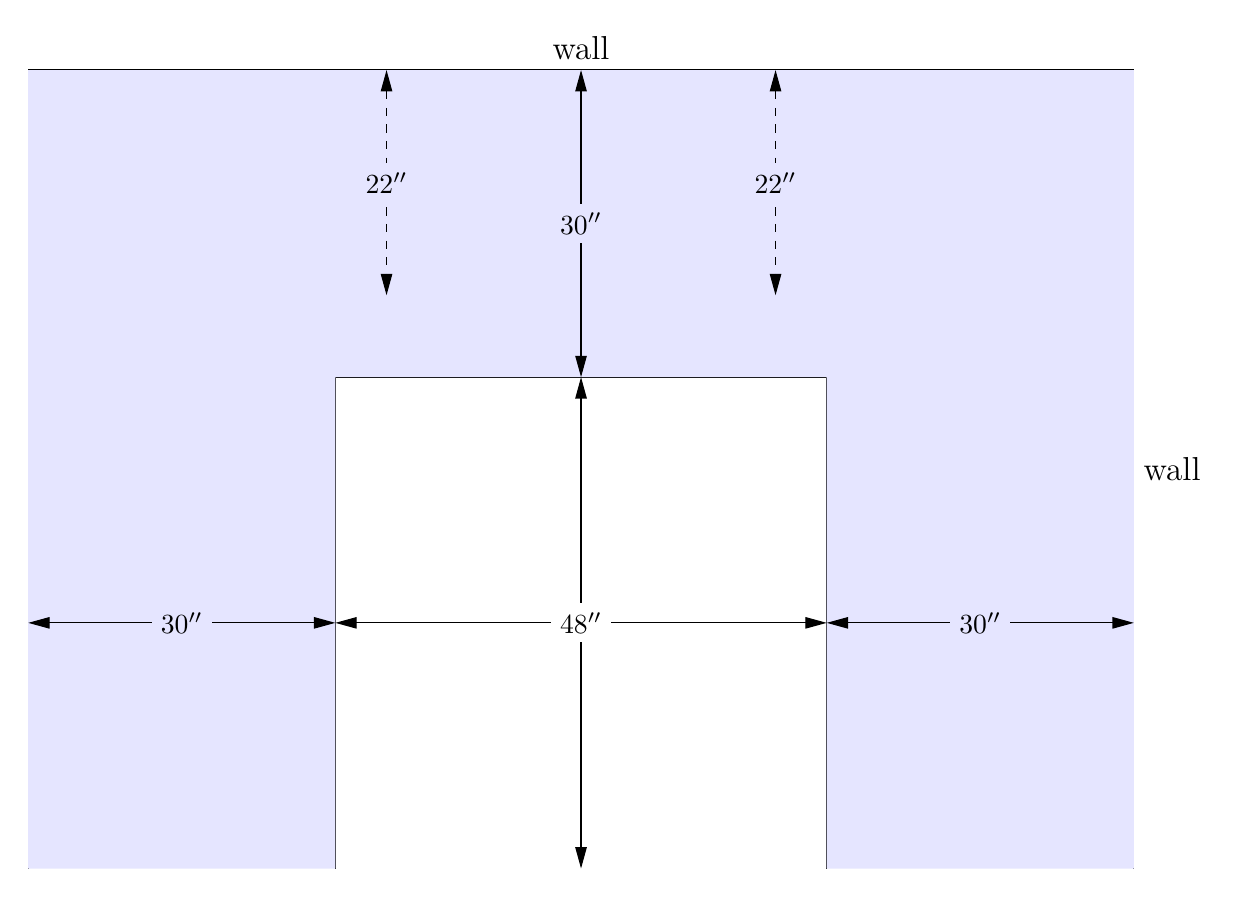
\begin{tikzpicture}[scale=0.13]
  % Define points.
  \coordinate   (p11) at (  0, 78);
    \coordinate (p14) at ( 35, 78);
    \coordinate (p15) at ( 54, 78);
    \coordinate (p16) at ( 73, 78);
    \coordinate (p19) at (108, 78);
  \coordinate   (p24) at ( 35, 67);
    \coordinate (p26) at ( 73, 67);
  \coordinate   (p35) at ( 54, 63);
  \coordinate   (p44) at ( 35, 56);
    \coordinate (p46) at ( 73, 56);
  \coordinate   (p53) at ( 30, 48);
    \coordinate (p55) at ( 54, 48);
    \coordinate (p57) at ( 78, 48);
  \coordinate   (p69) at (108, 39);
  \coordinate   (p71) at (  0, 24);
    \coordinate (p72) at ( 15, 24);
    \coordinate (p73) at ( 30, 24);
    \coordinate (p75) at ( 54, 24);
    \coordinate (p77) at ( 78, 24);
    \coordinate (p78) at ( 93, 24);
    \coordinate (p79) at (108, 24);
  \coordinate   (p81) at (  0,  0);
    \coordinate (p83) at ( 30,  0);
    \coordinate (p85) at ( 54,  0);
    \coordinate (p87) at ( 78,  0);
    \coordinate (p89) at (108,  0);
  % Put "wall" above drawing.
  \draw (p15) node[above] {\large wall};
  % Plot outer edge.
  \draw (p81) -- (p11) -- (p19) -- (p89);
  % Plot inner edge.
  \draw (p83) -- (p53) -- (p57) -- (p87);
  % Color the counter. 
  \fill[blue!10] (p81) -- (p11) -- (p19) -- (p89) -- (p87) -- (p57) -- (p53) -- (p83) -- cycle;
  % Vertical measurement lines.
  \draw[dashed, arrows = {Stealth[inset=0pt, angle=30:8pt]-Stealth[inset=0pt, angle=30:8pt]}]
    (p14) -- (p44);
  \draw (p24) node[fill=blue!10] {$22''$};
  \draw[arrows = {Stealth[inset=0pt, angle=30:8pt]-Stealth[inset=0pt, angle=30:8pt]}] (p15) -- (p55);
  \draw (p35) node[fill=blue!10] {$30''$};
  \draw[dashed, arrows = {Stealth[inset=0pt, angle=30:8pt]-Stealth[inset=0pt, angle=30:8pt]}]
    (p16) -- (p46);
  \draw (p26) node[fill=blue!10] {$22''$};
  \draw[arrows = {Stealth[inset=0pt, angle=30:8pt]-Stealth[inset=0pt, angle=30:8pt]}] (p55) -- (p85);
  % Horizontal measurement lines.
  \draw[arrows = {Stealth[inset=0pt, angle=30:8pt]-Stealth[inset=0pt, angle=30:8pt]}] (p71) -- (p73);
  \draw (p72) node[fill=blue!10] {$30''$};
  \draw[arrows = {Stealth[inset=0pt, angle=30:8pt]-Stealth[inset=0pt, angle=30:8pt]}] (p73) -- (p77);
  \draw (p75) node[fill=white] {$48''$};
  \draw[arrows = {Stealth[inset=0pt, angle=30:8pt]-Stealth[inset=0pt, angle=30:8pt]}] (p77) -- (p79);
  \draw (p78) node[fill=blue!10] {$30''$};
  % Put "wall" to the right of drawing.
  \draw (p69) node[right] {\large wall};
\end{tikzpicture}
\end{VerbatimOut}

\MyIO


\begin{VerbatimOut}{z.out}

\subsection{Fourier transform example}
\index{Fourier transform \TikZLogo\ example}
\todoindex{Fourier transform \TikZLogo\ example}
  
The Fourier transform decomposes a function
into the frequencies that make it up.
The inverse Fourier transformation combines the contributions
of all the different frequencies to recover the original function.

(Mark Senn {\tt\char'074}mark@purdue.edu{\tt\char'076} wrote sales@aavos.be on 2021-09-03
to ask permission
to use
\href{https://aavos.eu/glossary/fourier-transform/}{Fourier transform}
as the starting point
for an example \TikZLogo\ figure.  
Dominique Demurie {\tt\char'074}sales@aavos.be{\tt\char'076} replied
on 2021-09-06 with
``I think it is not an original drawing from us either.
We had it for years on our website,
but I cannot remember where we got it from.
We don't mind you using it for a thesis.'')

% Run this with
%     pdflatex --shell-escape t
% That makes the t.table.* files.
%
% See
%     https://ctan.math.washington.edu/tex-archive/graphics/pgf/base/doc/pgfmanual.pdf
%     PAGE    TOPIC
%      655    decorations.text library to draw text 
%     1221    animations
%
% for text decorations, which includes text along a path information.
% Also see
%     https://tex.stackexchange.com/questions/427454/tikz-3dplot-and-rotation-of-coordinates
%     https://tex.stackexchange.com/questions/67573/tikz-shift-and-rotate-in-3d
%     http://tug.ctan.org/graphics/pgf/contrib/tikz-3dplot/tikz-3dplot_documentation.pdf
%     https://tex.stackexchange.com/questions/45848/rotate-node-text-and-use-relative-positioning-in-tikz
  
% was scale = 2
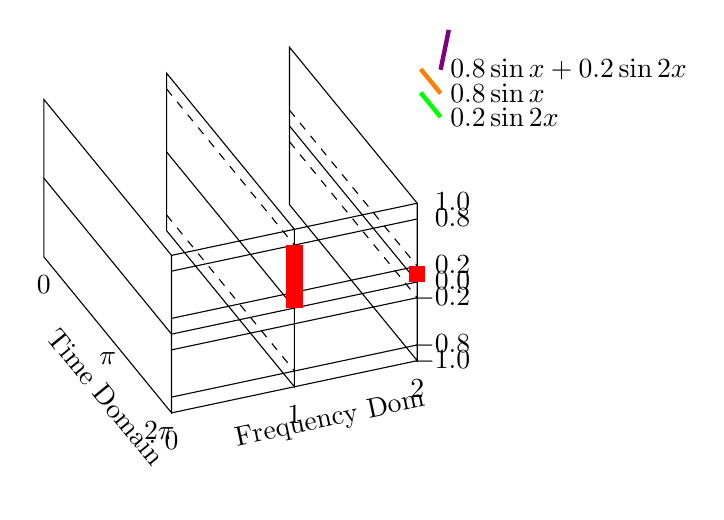
\begin{tikzpicture}[domain=0:6.283185, rotate around y=-55, scale=1]

  % total plot
  \begin{scope}[canvas is xy plane at z=0]
    \node[below=3pt] at (0,        -1) {0};
    \node[below=3pt] at (3.141593, -1) {$\pi$};
    \node[below=5pt] at (5.683185, -1) {$2\pi$};
    \draw[ultra thick,color=violet] plot[id=total,smooth] function{0.8*sin(x)+0.2*sin(8*x)};
    \draw[thin,color=black] (0,-1) -- (0,1) -- (6.283185,1) -- (6.283185,-1) -- cycle;
    \draw[thin,color=black] (0,0) -- (6.283185,0);
    \path[decorate,decoration={text along path,
% |\LARGE|
      text={Time Domain}}] (0.1,-2) -- (6.283185,-2); 
    % $s(t)$
  \end{scope}

  % tall plot
  \begin{scope}[canvas is xy plane at z=-1.5]
    \draw[dashed] (0,0.8) -- (6.283185,0.8);
    \draw[dashed] (0,-0.8) -- (6.283185,-0.8);
    \draw[thick,color=orange] plot[id=tall,smooth] function{0.8*sin(x)};
    \draw[thin,color=black] (0,-1) -- (0,1) -- (6.283185,1) -- (6.283185,-1) -- cycle;
    \draw[thin,color=black] (0,0) -- (6.283185,0);
  \end{scope}

  % short plot
  \begin{scope}[canvas is xy plane at z=-3.0]
    \draw[dashed] (0, 0.2) -- (6.283185,  0.2);
    \draw[dashed] (0,-0.2) -- (6.283185, -0.2);
    \draw[thick,color=green] plot[id=short,smooth] function{0.2*sin(2*x)};
    \draw[thin,color=black] (0,-1) -- (0,1) -- (6.283185,1) -- (6.283185,-1) -- cycle;
    \draw[thin,color=black] (0,0) -- (6.283185,0);
  \end{scope}

  % frequency plot
  \begin{scope}[canvas is zy plane at x=6.283185]
    \node[below=3pt] at ( 0.0,-1) {0};
    \node[below=3pt] at (-1.5,-1) {1};
    \node[below=3pt] at (-3.0,-1) {2};
    \draw[thin,color=black] (0,-1.0) -- (-3.0,-1.0);  \node[above=-9pt] at (-3.3,-1.0) {$-1.0$};
    \draw[thin,color=black] (0,-0.8) -- (-3.0,-0.8);  \node[above=-9pt] at (-3.3,-0.8) {$-0.8$};
    \draw[thin,color=black] (0,-0.2) -- (-3.0,-0.2);  \node[above=-9pt] at (-3.3,-0.2) {$-0.2$};
    \draw[thin,color=black] (0, 0.0) -- (-3.0, 0.0);  \node[above=-9pt] at (-3.3, 0.0) {$\phantom{-}0.0$};
    \draw[thin,color=black] (0, 0.2) -- (-3.0, 0.2);  \node[above=-9pt] at (-3.3, 0.2) {$\phantom{-}0.2$};
    \draw[thin,color=black] (0, 0.8) -- (-3.0, 0.8);  \node[above=-9pt] at (-3.3, 0.8) {$\phantom{-}0.8$};
    \draw[thin,color=black] (0, 1.0) -- (-3.0, 1.0);  \node[above=-9pt] at (-3.3, 1.0) {$\phantom{-}1.0$};
    \draw[line width=6pt,color=red] (-1.5,0) -- (-1.5,0.8);
    \draw[line width=6pt,color=red] (-3.0,0) -- (-3.0,0.2);
    \path[decorate,decoration={text along path,
% |\LARGE|
      text={Frequency Domain}}] (-0.8,-1.6) -- (-3.0,-1.6); 
    % $S(\omega)$
  \end{scope}

  %% legend
  %% Wolfram Language code:
  %%     In[1]:= ry[theta_] :=
  %%     {
  %%         {Cos[theta Degree],  0, Sin[theta Degree]},
  %%         {0,                  1, 0},
  %%         {-Sin[theta Degree], 0, Cos[theta Degree]}
  %%     }
  %%
  %%     ry[55] . {Pi, 0.7, -3.5}
  %%     # Out[] = {-1.06509, 0.7, -4.58096}
  %%     ry[55] . {(3/4)Pi, 0.7, -3.5}
  %%     # Out[] = {-1.51557, 0.7, -3.9376}

  \draw[ultra thick,color=violet] (2.45782, 1.7, -4.33538) -- (1.06509, 0.7, -4.58096);
    \node[right] at                                            (1.06509, 0.7, -4.58096) {$0.8\sin x + 0.2\sin 2x$};
  \draw[ultra thick,color=orange] ( 0.08509, 0.4, -4.58096) -- (1.06509, 0.4, -4.58096);
    \node[right] at                                            (1.06509, 0.4, -4.58096) {$0.8\sin x$};
  \draw[ultra thick,color=green]  ( 0.08509, 0.1, -4.58096) -- (1.06509, 0.1, -4.58096);
    \node[right] at                                            (1.06509, 0.1, -4.58096) {$0.2\sin 2x$};
\end{tikzpicture}
\end{VerbatimOut}

\MyIO


\begin{VerbatimOut}{z.out}

\subsection{Glider example}
\ix{Hirzel, Alex}
\index{glider \TikZLogo\ example}
\todoindex{glider \TikZLogo\ example}

The glider
is a pattern from the Game of Life,
and it's used as an emblem representing the hacker community.

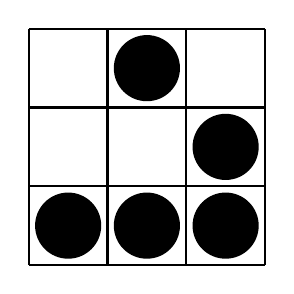
\begin{tikzpicture}[thick]
  \draw (0,0) grid (3,3);
  \foreach \c in {(0,0), (1,0), (2,0), (2,1), (1,2)}
    \fill \c + (0.5,0.5) circle (0.42);
\end{tikzpicture}
\end{VerbatimOut}

\MyIO


\begin{VerbatimOut}{z.out}


\subsection{Tree example}
\ix{???, ???}
\index{tree \TikZLogo\ example}
\todoindex{tree \TikZLogo\ example}

{
  \def\f#1#2{$\displaystyle\frac #1#2$}
  \begin{tikzpicture}%
  [%
    level 1/.style={sibling distance=60mm},
    level 2/.style={sibling distance=30mm},
    level 3/.style={sibling distance=15mm}
  ]
    \node {\f 11}
      child {node {$\displaystyle\frac 12$}
        child {node {\f 13}
          child {node {\f 14}}
          child {node {\f 48}}
        }
        child {node {\f 32}
          child {node {\f 35}}
          child {node {\f 52}}
        }
      }
      child {node {\f 21}
        child {node {\f 23}
          child {node {\f 25}}
          child {node {\f 53}}
        }
        child {node {\f 31}
          child {node {\f 34}}
          child {node {\f 41}}
        }
      };
  \end{tikzpicture}    
\end{VerbatimOut}

\MyIO


\begin{VerbatimOut}{z.out}
The node with value \f nd
\begin{inlinetable}
  \begin{tabular}{@{}llll@{}}
    \bfseries with additional conditions& \bfseries has& \bfseries with value\\
    \noalign{\vspace{2pt}}
    (none)&                     left child&     \f n{{n+d}}\\
    \noalign{\vspace{12pt}}
    (none)&                     right child&    \f {{n+d}}d\\
    \noalign{\vspace{12pt}}
    $n<d$&                      parent&         \f n{{d-n}}\\
    \noalign{\vspace{12pt}}
    $n=d$&                      no parent&      (not applicable)\\
    \noalign{\vspace{12pt}}
    $n>d$&                      parent&         \f {{n-d}}d\\
  \end{tabular}
\end{inlinetable}
\end{VerbatimOut}

\MyIO


\begin{VerbatimOut}{z.out}


\subsection{Yin and yang example}

This Yin and yang example was done by Thomas G. Kristensen \cite{kristensen}.
This is the ``traditional Taijitu symbol from Chinese philosophy''.
\ix{Kristensen, Thomas G.//Taijitu symbol//Yin and yang symbol}

\index{TikZ@\TikZLogo}  
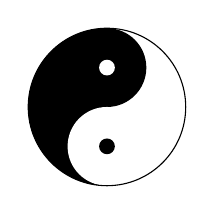
\begin{tikzpicture}
  % Yin and yang
  % Author: Thomas G. Kristensen
  
  % color one half of a unit circle                                              
  \begin{scope}
    \clip (0,0) circle (1cm);
    \fill[black] (0cm,1cm) rectangle (-1cm, -1cm);
  \end{scope}

  % fill heads                                                                   
  \fill[black] (0,0.5) circle (0.5cm);
  \fill[white] (0,-0.5) circle (0.5cm);

  % fill eyes                                                                    
  \fill[white] (0,0.5) circle (0.1cm);
  \fill[black] (0,-0.5) circle (0.1cm);

  % outer line                                                                   
  \draw (0,0) circle (1cm);

\end{tikzpicture}
\end{VerbatimOut}

\MyIO


\begin{VerbatimOut}{z.out}

\section{Wolfram Language (Mathematica uses this)}
\ix{Mathematica}
\ix{Wolfram Language}

\lightgreen{Wolfram Language can be set up to use \LaTeX\ fonts.}

\includegraphics{gr-mathematica.pdf}

This is the |misc/gr-mathematica.ma| input file
\MyI{misc/gr-mathematica.ma}

I typed, on Linux,
\Shell{math < gr-mathematica.ma}
in the |misc| subdirectory
to make the |graphics/gr-mathematica.pdf| output file.
\end{VerbatimOut}

\MyIO


% Ignore these references.
\ProvidesFile{ap-ignore-these-references.tex}[2022-05-16 ignore these references appendix]

\begin{VerbatimOut}{z.out}
\chapter{IGNORE THESE REFERENCES---THEY ARE WRONG}
\end{VerbatimOut}

\MyIO


\begin{VerbatimOut}{z.out}

You may have seen these references on the web.
Ignore them---they're wrong.

\noindent
\textbf{Purdue Online Writing Lab, IEEE Reference List}
\cite{owl}

The IEEE
(The world's largest technical professional organization
for the advancement
of technology)
has changed their references format from,
for example,

\noindent
\begin{tabular}{@{}ll@{}}
\noalign{\vspace*{6pt}}
  [1]& W. K. Chen, Linear Networks and Systems. Belmont, CA: Wadsworth Press,\\
  \multispan{2}{2003.\hfil}\\
\noalign{\vspace*{6pt}}
\noalign{\noindent to}
\noalign{\vspace*{6pt}}
  [1]& W. K. Chen, Linear Networks and Systems. Belmont, CA: Wadsworth Press,\\
  & 2003.\hfil\\
\noalign{\vspace*{6pt}}
\end{tabular}
See
\cite[page~2]{ieeedataport}.
\end{VerbatimOut}

\MyIO


% BL  @online{owl,
% BT  @misc{owl,
%     author  = {Purdue Online Writing Lab},
%     title   = {IEEE Reference List},
%     url     = {https://owl.purdue.edu/owl/research_and_citation/ieee_style/reference_list.html},
% BL  urldate = {2022-03-17},
% }
% 
% BL  @online{ieeedataport,
% BT  @misc{ieeedataport,
%     author  = {IEEEDataPort},
%     title   = {How too Cite References: IEEE Documentation Style},
%     url     = {https://ieee-dataport.org/sites/default/files/analysis/27/IEEE%20Citation%20Guidelines.pdf},
% BL  urldate = {2022-03-17},
% }  


% Logos.
\ProvidesFile{ap-logos.tex}[2022-07-11 logos appendix]

\begin{VerbatimOut}{z.out}
\chapter{LOGOS}

These logos are defined in |pa-logos.sty|:

\begin{inlinetable}
  \begin{tabular}{@{}ll@{}}
    \toprule
    \textbf{Input}& \textbf{Output}\\
    \midrule
    % From thesis.tex
    %     \newcommand{\tabularspace}{\noalign{\vspace*{2pt}}}
    % \tabularspace
    \noalign{\vspace{2pt}}
    |\AMSmathLogo|& \AMSmathLogo\\[2pt]
    |\BibLaTeXLogo|& \BibLaTeXLogo\\[2pt]
    |\BiberLogo|& \BiberLogo\\[2pt]
    |\CalligraphicAMSLaTeXLogo|& \CalligraphicAMSLaTeXLogo\\[2pt]
    |\CircuiTikZLogo|& \CircuiTikZLogo\\[2pt]
    |\CTANLogo|& \CTANLogo\\[2pt]
    |\LaTeXLogo|& \LaTeXLogo\\[2pt]
    |\LuaLaTeXLogo|& \LuaLaTeXLogo\\[2pt]
    |\METAFONTLogo|& \METAFONTLogo\\[2pt]
    |\METAPOSTLogo|& \METAPOSTLogo\\[2pt]
    |\MetaPostLogo|& \MetaPostLogo\\[2pt]
    |\NonCalligraphicAMSLaTeXLogo|& \NonCalligraphicAMSLaTeXLogo\\[2pt]
    |\PurdueThesisLogo|& \PurdueThesisLogo\\[2pt]
    |\PuThLogo|& \PuThLogo\\[2pt]
    |\siunitxLogo|& \siunitxLogo\\[2pt]
    |\TeXLogo|& \TeXLogo\\[2pt]
    |\TeXLiveLogo|& \TeXLiveLogo\\[2pt]
    |\TikZLogo|& \TikZLogo\\[2pt]
    |\TEXUsersGroupLogo|& \TeXUsersGroupLogo\\[2pt]
    |\TUGboatLogo|& \TUGboatLogo\\[2pt]
    \bottomrule
  \end{tabular}
\end{inlinetable}
\end{VerbatimOut}

\MyIO


% Numbers, units, and quantities.
\ProvidesFile{ap-numbers.tex}[2022-07-09 numbers, units, and etc. appendix]

%  Primary sources:
%      See https://www.bipm.org/utils/common/pdf/si-brochure/SI-Brochure-9-EN.pdf.
%      See https://www.nist.gov/pml/special-publication-811/nist-guide-si-chapter-4-two-classes-si-units-and-si-prefixes.
%
%  Notes:
%      See https://www.iso.org/standard/60241.html.

\begin{VerbatimOut}{z.out}
\chapter{NUMBERS, UNITS, AND ETC.}

The \siunitxLogo\ \LaTeX\ package
\cite{wright2022}
can be used
to correctly typeset
numbers,
units,
combined units,
quantities (numbers with units or combined units),
etc.
\end{VerbatimOut}

\MyIO


%xx Note to self: scientific prefixes, scientific suffixes, tables.
%xx
%xx \begin{VerbatimOut}{z.out}
%xx
%xx \section{Number Examples}
%xx \end{VerbatimOut}
%xx
%xx \MyIO
%xx
%xx \begin{VerbatimOut}{z.out}
%xx
%xx \section{Unit Examples}
%xx \end{VerbatimOut}
%xx
%xx \MyIO
%xx
%xx \noindent\begin{tabular}{@{}lll@{}}
%xx   \textbf{Input}& \textbf{Output}& \textbf{Comment}\\
%xx   \tabularspace
%xx   \verb+\si{\kg}+& \si{\kg}& kilogram\\
%xx   \verb+\si{\m}+& \si{\m}& meter\\
%xx   \verb+\si{\kg\per\m\squared}+&
%xx     \si{\kg\per\m\squared}&
%xx     \(= \si{\kg}/\si{\m\squared}\)\\
%xx \end{tabular}
%xx \end{VerbatimOut}
%xx
%xx \MyIO
%xx
%xx \begin{VerbatimOut}{z.out}
%xx
%xx \section{Combined Number and Unit Examples}
%xx \end{VerbatimOut}
%xx
%xx \MyIO
%xx
%xx \begin{VerbatimOut}{z.out}
%xx \begin{tabular}{@{}lll@{}}
%xx   \textbf{Input}& \textbf{Output}& \textbf{Comment}\\
%xx   \tabularspace
%xx   \verb+\SI{12}{\kg}+& \SI{12}{\kg}& 12 kilograms\\
%xx   \verb+\SI{34}{\m}+&  \SI{34}{\m}& 34 meters\\
%xx   % The next input line is too wide for the margins
%xx   % so I'm splitting it into pieces.
%xx   \verb+\SI{4.5e3}{\kg\per\m\squared}+&
%xx     \SI{4.5e3}{\kg\per\m\squared}&
%xx     \(= \num{4.5e3}\,\si{\kg}/\si{\m\squared}\)\\
%xx \end{tabular}
%xx \end{VerbatimOut}
%xx
%xx \MyIO
%xx
%xx \begin{VerbatimOut}{z.out}
%xx
%xx How many seconds are in a non-leap year that does not have any leap seconds?
%xx % I tried several things and couold not get \cancel to work with \per.
%xx % Mark Senn    2019-12-29
%xx \begin{align*}
%xx            \frac{\SI{365}{\cancel\d}}{\si{\y}}
%xx     \times \frac{\SI{24}{\cancel\h}}{\si{\cancel\d}}
%xx     \times \frac{\SI{60}{\cancel\min}}{\si{\cancel\h}}
%xx     \times \frac{\SI{60}{\s}}{\si{\cancel\min}}
%xx     % From http://www.emerson.emory.edu/services/latex/latex_119.html
%xx     %     Spacing in Math Mode
%xx     %     In a math environment, LaTeX ignores the spaces you type
%xx     %     and puts in the spacing that it thinks is best. LaTeX formats
%xx     %     mathematics the way it's done in mathematics texts. If you
%xx     %     want different spacing, LaTeX provides the following four
%xx     %     commands for use in math mode:
%xx     %         \; - a thick space
%xx     %         \: - a medium space
%xx     %         \, - a thin space
%xx     %         \! - a negative thin space
%xx     & = \num{31536000}\;\frac{\si{\s}}{\si{\y}}\\
%xx     & = \SI{31536000}{\s\per\y}\\
%xx     & \approx \SI{3e7}{\s\per\y}\\
%xx     & \approx \text{30 million\,}\si{\s\per\y}\\
%xx \end{align*}
%xx \end{VerbatimOut}
%xx
%xx \MyIO
%xx
%xx % Information in this section is consistent with [SIUNITX-20220607].
%xx % Checked on 2022-06-17.



\begin{VerbatimOut}{z.out}


\section{Numbers}
\end{VerbatimOut}

\MyIO


\begin{VerbatimOut}{z.out}

\subsection{Number Examples}

\begin{inlinetable}
  \begin{tabular}{@{}lll@{}}
    \toprule
    \textbf{Input}& \textbf{Output}& \textbf{Comment}\\
    \midrule
    |\num{3.45d-4}|&         \num{3.45d-4}\\
    |\num{-0.12345}|&        \num{-0.12345}&               note the small space after the |3|\\
    |\num{-0.1234}|&         \num{-0.1234}&                note no space between the |3| and |4|\\
    |\num{-.123}|&           \num{-.123}&                  the |0.| is inserted automatically\\
    |\num{.123}|&            \num{.123}&                   the |0.| is inserted automatically\\
    |\num{0.123}|&           \num{0.123}\\
    |\num{0.1234}|&          \num{0.1234}&                 note no space between the |3| and |4|\\
    |\num{0.12345}|&         \num{0.12345}&                note the small space after the |3|\\
    |\num{123}|&             \num{123}\\
    |\num{1234}|&            \num{1234}\\
    |\num{12345}|&           \num{12345}&                  note the small space after the |2|\\
    |\num{2e4}|&             \num{2e4}\\
    |\num{e5}|&              \num{e5}\\
    |\num{2.34567e6}|&       \num{2.34567e6}&              note the small space after the |5|\\[6pt]
    |\numlist{10;30;50;70}|& \numlist{10;30;50;70}\\[6pt]
    |\numproduct{10 x 20}|&  \numproduct{10 x 20}\\[6pt]
    |\numrange{10}{30}|&     \numrange{10}{30}\\[6pt]
    |\complexnum{-4}|&       \complexnum{-4}\\
    |\complexnum{-3-2i}|&    \complexnum{-3-2i}\\
    |\complexnum{2+3i}|&     \complexnum{2+3i}\\
    |\complexnum{4+-5i}|&    \complexnum{4+-5i}\\
    \bottomrule
  \end{tabular}
\end{inlinetable}
\end{VerbatimOut}

\MyIO


\begin{VerbatimOut}{z.out}


\section{Units}

A unit consists of an optional prefix
followed by a unit.
\end{VerbatimOut}

\MyIO


\begin{VerbatimOut}{z.out}

\subsection{Binary Prefixes}

These binary prefixes are defined by \siunitxLogo\ and
are used for units related to computers,
data storage,
data transmission,
etc.
  
\begin{inlinetable}
  % Define a math mode version of "r" column type.
  \newcolumntype{m}{>{$}l<{$}}%
  \begin{tabular}{@{}mllll@{}}
    \toprule
    \textbf{Factor}& \textbf{Prefix}& \textbf{Pronounciation}& \textbf{Command}& \textbf{Symbol}\\
    \midrule
    2^{10}& kibi& kilobee& |\kibi|& \unit{\kibi\nounit}\\
    2^{20}& mebi& megabee& |\mebi|& \unit{\mebi\nounit}\\
    2^{30}& gibi& gigabee& |\gibi|& \unit{\gibi\nounit}\\
    2^{40}& tebi& terabee& |\tebi|& \unit{\tebi\nounit}\\
    2^{50}& pebi& pebibee& |\pebi|& \unit{\pebi\nounit}\\
    2^{60}& exbi& exbibee& |\exbi|& \unit{\exbi\nounit}\\
    2^{70}& zebi& zetabee& |\zebi|& \unit{\zebi\nounit}\\
    2^{80}& yobi& yobibee& |\yobi|& \unit{\yobi\nounit}\\
    \bottomrule
  \end{tabular}
\end{inlinetable}
\end{VerbatimOut}

\MyIO


\begin{VerbatimOut}{z.out}

\subsection{Decimal Prefixes}

These decimal prefixes are used for units that are usually not
related to computers.

\begin{inlinetable}
  \newcolumntype{m}{>{$}l<{$}}%
  \begin{tabular}{@{}mlll@{}}
    \toprule
    \textbf{Factor}& \textbf{Prefix}& \textbf{Command}& \textbf{Symbol}\\
    \midrule
    10^{-24}& yocto& |\yocto|& \unit{\yocto\nounit}\\
    10^{-21}& zepto& |\zepto|& \unit{\zepto\nounit}\\
    10^{-18}& atto&  |\atto|&  \unit{\atto\nounit}\\
    10^{-15}& femto& |\femto|& \unit{\femto\nounit}\\
    10^{-12}& pico&  |\pico|&  \unit{\pico\nounit}\\
    10^{ -9}& nano&  |\nano|&  \unit{\nano\nounit}\\
    10^{ -6}& micro& |\micro|& \unit{\micro\nounit}\\
    10^{ -3}& milli& |\milli|& \unit{\milli\nounit}\\
    10^{ -2}& centi& |\centi|& \unit{\centi\nounit}\\
    10^{ -1}& deci&  |\deci|&  \unit{\deci\nounit}\\
    10^{  1}& deca&  |\deca|&  \unit{\deca\nounit}\\   % or \deka
    10^{  2}& hecto& |\hecto|& \unit{\hecto\nounit}\\
    10^{  3}& kilo&  |\kilo|&  \unit{\kilo\nounit}\\
    10^{  6}& mega&  |\mega|&  \unit{\mega\nounit}\\
    10^{  9}& giga&  |\giga|&  \unit{\giga\nounit}\\
    10^{ 12}& tera&  |\tera|&  \unit{\tera\nounit}\\
    10^{ 15}& peta&  |\peta|&  \unit{\peta\nounit}\\
    10^{ 18}& exa&   |\exa|&   \unit{\exa\nounit}\\
    10^{ 21}& zetta& |\zetta|& \unit{\zetta\nounit}\\
    10^{ 24}& yotta& |\yotta|& \unit{\yotta\nounit}\\
    \bottomrule
  \end{tabular}
\end{inlinetable}
\end{VerbatimOut}

\MyIO


\begin{VerbatimOut}{z.out}

Here is the complete list of units defined
by the \siunitxLogo\ package:

{
  \ZZbaselinestretch{1}
  % See
  %     https://tex.stackexchange.com/questions/100351/siunitxs-micro-symbol-has-serif
  % for solution to \micro using wrong font.
  \newcommand{\q}{\quad}
  \begin{longtable}{@{}lllll@{}}%
      \caption{Units}\\
      \textbf{Name}& \textbf{Input}& \textbf{Output}& \textbf{Input}& \textbf{Output}\\[6pt]
    \endfirsthead
      \caption[]{~\emph{continued}}\\
      \textbf{Name}& \textbf{Input}& \textbf{Output}& \textbf{Input}& \textbf{Output}\\[6pt]
    \endhead
      \multicolumn{4}{@{}c@{}}{\emph{continued on next page}}%
    \endfoot
    \endlastfoot
    % Normally I'd indent the following lines but that makes them
    % to wide to print the input within the margins.
    ampere&               |\A|&    \unit{\A}&    |\ampere|&             \unit{\ampere}\\
    \q picoampere&        |\pA|&   \unit{\pA}&   |\pico\ampere|&        \unit{\pico\ampere}\\
    \q nanoampere&        |\nA|&   \unit{\nA}&   |\nano\ampere|&        \unit{\nano\ampere}\\
    \q microampere&       |\uA|&   \unit{\uA}&   |\micro\ampere|&       \unit{\micro\ampere}\\
    \q milliampere&       |\mA|&   \unit{\mA}&   |\milli\ampere|&       \unit{\milli\ampere}\\
    \q kiloampere&        |\kA|&   \unit{\kA}&   |\kilo\ampere|&        \unit{\kilo\ampere}\\[6pt]
    astronomical unit&    &        &             |\astronomicalunit|&   \unit{\astronomicalunit}\\[6pt]
    becquerel&            &        &             |\becquerel|&          \unit{\becquerel}\\[6pt]
    bel&                  &        &             |\bel|&                \unit{\bel}\\
    \q decibel&           |\dB|&   \unit{\dB}&   |\decibel|&            \unit{\decibel}\\[6pt]
    bit&                  &        &             |\bit|&                \unit{\bit}\\[6pt]
    byte&                 &        &             |\byte|&               \unit{\byte}\\[6pt]
    candela&              &        &             |\candela|&            \unit{\candela}\\[6pt]
    coulomb&              |\C|&    \unit{\C}&    |\coulomb|&            \unit{\coulomb}\\
    \q nanocoulomb&       |\nC|&   \unit{\nC}&   |\nano\coulomb|&       \unit{\nano\coulomb}\\
    \q microcoulomb&      |\uC|&   \unit{\uC}&   |\micro\coulomb|&      \unit{\micro\coulomb}\\
    \q millicoulomb&      |\mC|&   \unit{\mC}&   |\milli\coulomb|&      \unit{\milli\coulomb}\\[6pt]
    dalton&               &        &             |\dalton|&             \unit{\dalton}\\[6pt]
    day&                  &        &             |\day|&                \unit{\day}\\[6pt]
    degree (plane angle)& &        &             |\degree|&             \unit{\degree}\\
    \q minute&            &        &             |\arcminute|&          \unit{\arcminute}\\
    \q second&            &        &             |\arcsecond|&          \unit{\arcsecond}\\[6pt]
    degree Celsius&       &        &             |\degreeCelsuis|&      \unit{\degreeCelsius}\\[6pt]
    electronvolt&         |\eV|&   \unit{\eV}&   |\electronvolt|&       \unit{\electronvolt}\\
    \q millielectronvolt& |\meV|&  \unit{\meV}&  |\milli\electronvolt|& \unit{\milli\electronvolt}\\
    \q kiloelectronvolt&  |\keV|&  \unit{\keV}&  |\kilo\electronvolt|&  \unit{\kilo\electronvolt}\\
    \q megaelectronvolt&  |\MeV|&  \unit{\MeV}&  |\mega\electronvolt|&  \unit{\mega\electronvolt}\\
    \q gigaelectronvolt&  |\GeV|&  \unit{\GeV}&  |\giga\electronvolt|&  \unit{\giga\electronvolt}\\
    \q teraelectronvolt&  |\TeV|&  \unit{\TeV}&  |\tera\electronvolt|&  \unit{\tera\electronvolt}\\[6pt]
    farad&                |\F|&    \unit{\F}&    |\farad|&              \unit{\farad}\\
    \q femtofarad&        |\fF|&   \unit{\fF}&   |\femto\farad|&        \unit{\femto\farad}\\
    \q picofarad&         |\pF|&   \unit{\pF}&   |\pico\farad|&         \unit{\pico\farad}\\
    \q nanofarad&         |\nF|&   \unit{\nF}&   |\nano\farad|&         \unit{\nano\farad}\\
    \q microfarad&        |\uF|&   \unit{\uF}&   |\micro\farad|&        \unit{\micro\farad}\\[6pt]
    gram&                 |\g|&    \unit{\g}&    |\gram|&               \unit{\gram}\\
    \q femtogram&         |\fg|&   \unit{\fg}&   |\femto\gram|&         \unit{\femto\gram}\\
    \q picogram&          |\pg|&   \unit{\pg}&   |\pico\gram|&          \unit{\pico\gram}\\
    \q nanogram&          |\ng|&   \unit{\ng}&   |\nano\gram|&          \unit{\nano\gram}\\
    \q microgram&         |\ug|&   \unit{\ug}&   |\micro\gram|&         \unit{\micro\gram}\\
    \q milligram&         |\mg|&   \unit{\mg}&   |\milli\gram|&         \unit{\milli\gram}\\
    \q kilogram&          |\kg|&   \unit{\kg}&   |\kilogram|&           \unit{\kilogram}\\
    &                     &        &             |\kilo\gram|&          \unit{\kilo\gram}\\[6pt]
    gray&                 &        &             |\gray|&               \unit{\gray}\\[6pt]
    hectare&              &        &             |\hectare|&            \unit{\hectare}\\[6pt]
    henry&                |\H|&    \unit{\H}&    |\henry|&              \unit{\henry}\\
    \q femtohentry&       |\fH|&   \unit{\fH}&   |\femto\henry|&        \unit{\femto\henry}\\
    \q picohentry&        |\pH|&   \unit{\pH}&   |\pico\henry|&         \unit{\pico\henry}\\
    \q nanohentry&        |\nH|&   \unit{\nH}&   |\nano\henry|&         \unit{\nano\henry}\\
    \q microhentry&       |\uH|&   \unit{\uH}&   |\micro\henry|&        \unit{\micro\henry}\\
    \q millihentry&       |\mH|&   \unit{\mH}&   |\milli\henry|&        \unit{\milli\henry}\\[6pt]
    hertz&                |\Hz|&   \unit{\Hz}&   |\hertz|&              \unit{\hertz}\\
    \q millihertz&        |\mHz|&  \unit{\mHz}&  |\milli\hertz|&        \unit{\milli\hertz}\\
    \q kilohertz&         |\kHz|&  \unit{\kHz}&  |\kilo\hertz|&         \unit{\kilo\hertz}\\
    \q megahertz&         |\MHz|&  \unit{\MHz}&  |\mega\hertz|&         \unit{\mega\hertz}\\
    \q gigahertz&         |\GHz|&  \unit{\GHz}&  |\giga\hertz|&         \unit{\giga\hertz}\\
    \q terahertz&         |\THz|&  \unit{\THz}&  |\tera\hertz|&         \unit{\tera\hertz}\\[6pt]
    hour&                 &        &             |\hour|&               \unit{\hour}\\[6pt]
    joule&                |\J|&    \unit{\J}&    |\joule|&              \unit{\joule}\\
    \q microjoule&        |\uJ|&   \unit{\uJ}&   |\micro\joule|&        \unit{\micro\joule}\\
    \q millijoule&        |\mJ|&   \unit{\mJ}&   |\milli\joule|&        \unit{\milli\joule}\\
    \q kilojoule&         |\kJ|&   \unit{\kJ}&   |\kilo\joule|&         \unit{\kilo\joule}\\
    \q megajoule&         &        &             |\mega\joule|&         \unit{\mega\joule}\\[6pt]
    katal&                &        &             |\katal|&              \unit{\katal}\\[6pt]
    kelvin&               |\K|&    \unit{\K}&    |\kelvin|&             \unit{\kelvin}\\[6pt]
    kilowatt hour&        |\kWh|&  \unit{\kWh}&  \\[6pt]
    liter&                |\L|&    \unit{\L}&    |\liter|&              \unit{\liter}\\
    \q microliter&        |\uL|&   \unit{\uL}&   |\micro\liter|&        \unit{\micro\liter}\\
    \q milliliter&        |\mL|&   \unit{\mL}&   |\milli\liter|&        \unit{\milli\liter}\\
    \q hectoliter&        |\hL|&   \unit{\hL}&   |\hecto\liter|&        \unit{\hecto\liter}\\[6pt]
    lumen&                &        &             |\lumen|&              \unit{\lumen}\\[6pt]
    lux&                  &        &             |\lux|&                \unit{\lux}\\[6pt]
    meter&                |\m|&    \unit{\m}&    |\meter|&              \unit{\meter}\\
    \q picometer&         |\pm|&   \unit{\pm}&   |\pico\meter|&         \unit{\pico\meter}\\
    \q nanometer&         |\nm|&   \unit{\nm}&   |\nano\meter|&         \unit{\nano\meter}\\
    \q micrometer&        |\um|&   \unit{\um}&   |\micro\meter|&        \unit{\micro\meter}\\
    \q millimeter&        |\mm|&   \unit{\mm}&   |\milli\meter|&        \unit{\milli\meter}\\
    \q centimeter&        |\cm|&   \unit{\cm}&   |\centi\meter|&        \unit{\centi\meter}\\
    \q decimeter&         |\dm|&   \unit{\dm}&   |\deci\meter|&         \unit{\deci\meter}\\
    \q kilometer&         |\km|&   \unit{\km}&   |\kilo\meter|&         \unit{\kilo\meter}\\[6pt]
    minute (time)&        |\min|&  \unit{\min}&  |\minute|&             \unit{\minute}\\[6pt]
    mole&                 |\mol|&  \unit{\mol}&  |\mole|&               \unit{\mole}\\
    \q femtomole&         |\fmol|& \unit{\fmol}& |\femto\mole|&         \unit{\femto\mole}\\
    \q picomole&          |\pmol|& \unit{\pmol}& |\pico\mole|&          \unit{\pico\mole}\\
    \q nanomole&          |\nmol|& \unit{\nmol}& |\nano\mole|&          \unit{\nano\mole}\\
    \q micromole&         |\umol|& \unit{\umol}& |\micro\mole|&         \unit{\micro\mole}\\
    \q millimole&         |\mmol|& \unit{\mmol}& |\milli\mole|&         \unit{\milli\mole}\\
    \q kilomole&          |\kmol|& \unit{\kmol}& |\kilo\mole|&          \unit{\kilo\mole}\\[6pt]
    neper&                &        &             |\neper|&              \unit{\neper}\\[6pt]
    newton&               |\N|&    \unit{\N}&    |\newton|&             \unit{\newton}\\
    \q millinewton&       |\mN|&   \unit{\mN}&   |\milli\newton|&       \unit{\milli\newton}\\
    \q kilonewton&        |\kN|&   \unit{\kN}&   |\kilo\newton|&        \unit{\kilo\newton}\\
    \q meganewton&        |\MN|&   \unit{\MN}&   |\mega\newton|&        \unit{\mega\newton}\\[6pt]
    ohm&                  &        &             |\ohm|&                \unit{\ohm}\\
    \q milliohm&          |\mohm|& \unit{\mohm}& |\milli\ohm|&          \unit{\milli\ohm}\\
    \q kiloohm&           |\kohm|& \unit{\kohm}& |\kilo\ohm|&           \unit{\kilo\ohm}\\
    \q megaohm&           |\Mohm|& \unit{\Mohm}& |\mega\ohm|&           \unit{\mega\ohm}\\[6pt]
    pascal&               |\Pa|&   \unit{\Pa}&   |\pascal|&             \unit{\pascal}\\
    \q kilopascal&        |\kPa|&  \unit{\kPa}&  |\kilo\pascal|&        \unit{\kilo\pascal}\\
    \q megapascal&        |\MPa|&  \unit{\MPa}&  |\mega\pascal|&        \unit{\mega\pascal}\\
    \q gigapascal&        |\GPa|&  \unit{\GPa}&  |\giga\pascal|&        \unit{\giga\pascal}\\[6pt]
    percent&              &        &             |\percent|&            \unit{\percent}\\[6pt]
    radian&               &        &             |\radian|&             \unit{\radian}\\[6pt]
    second&               |\s|&    \unit{\s}&    |\second|&             \unit{\second}\\
    \q attosecond&        |\as|&   \unit{\as}&   |\atto\second|&        \unit{\as}\\
    \q femtosecond&       |\fs|&   \unit{\fs}&   |\femto\second|&       \unit{\fs}\\
    \q picosecond&        |\ps|&   \unit{\ps}&   |\pico\second|&        \unit{\ps}\\
    \q nanosecond&        |\ns|&   \unit{\ns}&   |\nano\second|&        \unit{\ns}\\
    \q microsecond&       |\us|&   \unit{\us}&   |\micro\second|&       \unit{\us}\\
    \q millisecond&       |\ms|&   \unit{\ms}&   |\milli\second|&       \unit{\ms}\\[6pt]
    siemens&              &        &             |\siemens|&            \unit{\siemens}\\[6pt]
    sievert&              &        &             |\sievert|&            \unit{\sievert}\\[6pt]
    steradian&            &        &             |\steradian|&          \unit{\steradian}\\[6pt]
    tesla&                &        &             |\tesla|&              \unit{\tesla}\\[6pt]
    tonne (metric ton)&   &        &             |\tonne|&              \unit{\tonne}\\[6pt]
    volt&                 |\V|&    \unit{\V}&    |\volt|&               \unit{\volt}\\
    \q picovolt&          |\pV|&   \unit{\pV}&   |\pico\volt|&          \unit{\pico\volt}\\
    \q nanovolt&          |\nV|&   \unit{\nV}&   |\nano\volt|&          \unit{\nano\volt}\\
    \q microvolt&         |\uV|&   \unit{\uV}&   |\micro\volt|&         \unit{\micro\volt}\\
    \q millivolt&         |\mV|&   \unit{\mV}&   |\milli\volt|&         \unit{\milli\volt}\\
    \q kilovolt&          |\kV|&   \unit{\kV}&   |\kilo\volt|&          \unit{\kilo\volt}\\[6pt]
    watt&                 |\W|&    \unit{\W}&    |\watt|&               \unit{\watt}\\
    \q nanowatt&          |\nW|&   \unit{\nW}&   |\nW|&                 \unit{\nano\watt}\\
    \q microwatt&         |\uW|&   \unit{\uW}&   |\micro\watt|&        \unit{\micro\watt}\\
    \q milliwatt&         |\mW|&   \unit{\mW}&   |\milli\watt|&        \unit{\milli\watt}\\
    \q kilowatt&          |\kW|&   \unit{\kW}&   |\kilo\watt|&         \unit{\kilo\watt}\\
    \q megawatt&          |\MW|&   \unit{\MW}&   |\mega\watt|&         \unit{\mega\watt}\\
    \q gigawatt&          |\GW|&   \unit{\GW}&   |\giga\watt|&         \unit{\giga\watt}\\[6pt]
    weber&                &        &             |\weber|&             \unit{\weber}\\
  \end{longtable}
}
\end{VerbatimOut}

\MyIO


\begin{VerbatimOut}{z.out}

\subsection{Unit Examples}

\begin{inlinetable}
  \begin{tabular}{@{}ll@{}}
    \toprule
    \textbf{Input}& \textbf{Output}\\
    \midrule
    |\unit{\meter}|&       \unit{\meter}\\
    |\unit{\m}|&           \unit{\m}\\
    |\unit{m}|&            \unit{m}\\[6pt]
    |\unit{\milli\meter}|& \unit{\milli\meter}\\
    |\unit{\mm}|&          \unit{\mm}\\
    |\unit{mm}|&           \unit{mm}\\
    \bottomrule
  \end{tabular}
\end{inlinetable}
\end{VerbatimOut}

\MyIO


\begin{VerbatimOut}{z.out}
  
\subsection{Defining your own unit}

% Define \c as a unit for the speed of light.
\DeclareSIUnit{\c}{\text{c}}
The speed of light in a vacuum (\unit{\c}) is defined as \qty{299792457}{m\per s}
\cite{wikipedia-speed-of-light}.
\end{VerbatimOut}

\MyIO


\begin{VerbatimOut}{z.out}


\section{Combined Unit}

Units can be combined to make a combined unit.
|\NE| (negative exponent)
and |\PE| (positive exponent)
are defined in PurdueThesis.cls.
\end{VerbatimOut}

\MyIO


\begin{VerbatimOut}{z.out}

\subsection{Combined Unit Examples}

\begin{inlinetable}
  \begin{tabular}{@{}ll@{}}
    \toprule
    \textbf{Input}& \textbf{Output}\\
    \midrule
    |\unit{\meter\per\second}|&   \unit{\meter\per\second}\\
    |\unit{\m\per\s}|&            \unit{\m\per\s}\\
    |\unit{m.s^{-1}}|&            \unit{m.s^{-1}}\\
    |\unit{m.s\NE1}|&             \unit{m.s\NE1}\\[6pt]
    |\unit{m.s^2}|&               \unit{m.s^2}\\
    |\unit{m.s\PE2}|&             \unit{m.s\PE2}\\
    \bottomrule
  \end{tabular}
\end{inlinetable}
\end{VerbatimOut}

\MyIO


\begin{VerbatimOut}{z.out}


\section{Quantity}

A quantity consists of a number with a unit or combined units.

\subsection{Quantity Examples}

\begin{inlinetable}
  \begin{tabular}{@{}ll@{}}
    \toprule
    \textbf{Input}& \textbf{Output}\\
    \midrule
    |\qty{2}{\meter}|&            \qty{2}{\meter}\\
    |\qty{3}{\m}|&                \qty{3}{\m}\\
    |\qty{4}{m}|&                 \qty{4}{m}\\[6pt]
    |\qty{2}{\meter\per\second}|& \qty{2}{\meter\per\second}\\
    |\qty{3}{\m\per\s}|&          \qty{3}{\m\per\s}\\
    |\qty{4}{m.s^{-1}}|&          \qty{4}{m.s^{-1}}\\
    |\qty{5}{m.s\NE1}|&           \qty{5}{m.s\NE1}\\
    \bottomrule
  \end{tabular}
\end{inlinetable}
\end{VerbatimOut}

\MyIO


\begin{VerbatimOut}{z.out}

Using text math mode
|\(|\ldots|\)|
so spacing around equal signs is correct:\\
\(\qty{1}{W} = \qty{1}{J.s\NE1} = \qty{1}{kg.m\PE2.s\NE3}\)
\end{VerbatimOut}

\MyIO


\begin{VerbatimOut}{z.out}

The gravitation constant,
\(G\),
is approximately
\qty{6.674e-11}{m\PE3.kg\NE1.s\NE2}
\cite{wikipedia-gravitational-constant}.
\end{VerbatimOut}

\MyIO


\begin{VerbatimOut}{z.out}

The earth's gravitation acceleration is
\qty{9.80655}{m.s\NE2}
\cite{wikipedia-gravitational-acceleration}.
\end{VerbatimOut}

\MyIO


\begin{VerbatimOut}{z.out}


\section{Etc.}

\subsection{Angles}

\begin{inlinetable}
  \begin{tabular}{@{}lll@{}}
    \toprule
    \textbf{Input}& \textbf{Output}& \textbf{Comment}\\
    \midrule
    |-\ang{10}|&    -\ang{10}\\
    |\ang{;;3}|&    \ang{;;3}\\
    |\ang{;2;}|&    \ang{;2}\\
    |\ang{1}|&      \ang{1}\\
    |\ang{1;2}|&    \ang{1;2}\\
    |\ang{1;2;3}|&  \ang{1;2;3}\\
    |\ang{10}|&     \ang{10}\\
    \bottomrule
  \end{tabular}
\end{inlinetable}
\end{VerbatimOut}

\MyIO


\begin{VerbatimOut}{z.out}

\subsection{Cancel}

Using |\textstyle| size:
\unit[per-mode = fraction]
{\cancel\kilogram\meter\per\cancel\kilogram\per\second}
\end{VerbatimOut}

\MyIO


\begin{VerbatimOut}{z.out}

Using |\displaystyle| size:
{
  \(
    \displaystyle
    \unit[per-mode = fraction]%
    {\cancel\kilogram\meter\per\cancel\kilogram\per\second}
  \)
}
\end{VerbatimOut}

\MyIO


\begin{VerbatimOut}{z.out}
  
I first tried to do this using the \siunitxLogo\ |\per| command
but couldn't figure it out.
I decided to demonstrate how to do this without using SI unit abbreviations.
\begin{align}
          \frac {365\,\cancel{\textrm{day}}}    {\textrm{year}}
  \times  \frac {24\,\cancel{\textrm{hour}}}    {\cancel{\textrm{day}}}
  \times  \frac {60\,\cancel{\textrm{minute}}}  {\cancel{\textrm{hour}}}
  \times  \frac {60\,\textrm{\textrm{second}}}  {\cancel{\textrm{minute}}}
  & = 31,536,000 \textrm{ seconds/year}\nonumber\\
  & = \qty{31536000}{s.y\NE1}\quad\text{(in SI units)}\nonumber\\
  & \approx \textrm{32 million seconds/year}\nonumber
\end{align}
\end{VerbatimOut}

\MyIO


% TODO:
% Figure out how to format this and add it to the document.
% To estimate the number of digits in the answer:
% 365 -> 3 count all digits in first number
% 24 -> 1  count all digits and subtract one if first digit is 1 through 4
% 60 -> 2
% 60 -> 2


% The International System of Units (SI)
% https://www.bipm.org/en/measurement-units/

% The International System of Units (SI): Defining constants
% https://www.bipm.org/en/measurement-units/si-defining-constants

% The International System of Units (SI): Base units
% https://www.bipm.org/en/measurement-units/si-base-units


%xx \begin{VerbatimOut}{z.out}
%xx
%xx {%
%xx   \ZZbaselinestretch{1}
%xx   \newcommand\vsp{\noalign{\vspace*{6pt}}}
%xx   % From
%xx   % https://tex.stackexchange.com/questions/31508/flushleft-with-p-option-in-tabular
%xx   %     It's necessary to use the \arraybackslash in the last column,
%xx   %     otherwise \\ would not end the table row.  You can use \newline
%xx   %     to end lines in the last column cells (and the regular \\ in
%xx   %     the other column cells).
%xx   %     ...
%xx   %     If you need it often, consider defining a new column type using
%xx   %     array features, as I did here:
%xx   %         \newcolumntype{P}[1]{>{\raggedright\arraybackslash}p{#1}}
%xx   \newcolumntype{P}[1]{>{\raggedright\arraybackslash}p{#1}}%
%xx % \begin{longtable}{@{}P{1.4in}P{1in}llP{1.8in}@{}}
%xx % \begin{longtable}{@{}P{1in}P{1in}llP{1.8in}@{}}
%xx % \begin{longtable}{@{}P{1.2in}P{1in}llP{1.8in}@{}}
%xx % \begin{longtable}{@{}P{90.72pt}P{1in}llP{1.8in}@{}}  % 1.2in (86.72pt) + 4pt = 90.72pt
%xx   \begin{longtable}{@{}P{1.4in}P{1in}llP{1.8in}@{}}% 1.2in (86.72pt) + 4pt = 90.72pt
%xx     % \aa ngstr\"om&
%xx     %   length&
%xx     %   \si{\AA}&
%xx     %   \verb+\si{\AA}+&
%xx     %   \SI{e-10}{\m}\\
%xx     bar&
%xx       pressure&
%xx       \si{\bar}&
%xx       \verb+\si{\bar}+&
%xx       \SI{e-5}{\Pa}\\
%xx     \quad millibar&
%xx       \ditto&
%xx       \si{\mbar}&
%xx       \verb+\si{\mbar}+&
%xx       \SI{e-3}{\bar}\\
%xx     speed of light&
%xx       speed&
%xx       \si{\clight}&
%xx       \verb+\si{\clight}+&
%xx       \SI{299792458}{\m\per\s}\\
%xx %   temperatures
%xx %
%xx %       \degreeCelsius
%xx %       \celsius
%xx %
%xx %       range
%xx %           \SIrange{1}{5}{\metre}
%xx %           \SIrange{1}{5}{\milli\metre}
%xx %
%xx %
%xx %   numbers
%xx %   -10^{10}           \num{-e10}
%xx %                      \num{12345.67890}
%xx %                      \num{1+-2i}
%xx %                      \num{.3.45}
%xx %
%xx %       \celsius


% Resources.
\ProvidesFile{ap-resources.tex}[2022-05-16 resources appendix]

\begin{VerbatimOut}{z.out}
\chapter{RESOURCES}

Books:
\begin{itemize}
  \item
  \citetitle{kottwitz2021}, second edition, \cite{kottwitz2021}.
\end{itemize}
  
\noindent
From the
IEEE Author Center
\cite{ieee-author-center}
\begin{itemize}
  \item
    The
    IEEE Editorial Style Manual for Authors
    \cite{ieee-editorial-style-manual-for-authors}
    contains a formal set of editorial guidelines.
  \item
    Editing Mathematics
    \cite{editing-mathematics}
    illustrates how to do mathematics.
  \item
    The
    IEEE Reference Guide
    \cite{ieee-reference-guide}
    outlines how to cite references.
\end{itemize}

\noindent
Question and Answer site:
\begin{itemize}
  \item
    \TeX\ -- \LaTeX\ Stack Exchange
    is a question and answer site
    for users of
    \TeX,
    \LaTeX,
    and related typesetting systems
    \cite{tex-stackexchange}.
\end{itemize}
\end{VerbatimOut}

\MyIO


% Tables.
\ProvidesFile{ap-tables.tex}[2022-05-16 tables appendix]

\begin{VerbatimOut}{z.out}
\chapter{TABLES}
\ix{table}
\end{VerbatimOut}

\MyIO


% \newlength{\ta}
% \newlength{\tb}
% \newlength{\tc}
% 
% \settowidth{\ta}{\vbox{\hbox{Money}\hbox{Market}}}
% \settowidth{\tb}{\vbox{\hbox{Stocks}\hbox{and}\hbox{Bonds}}}
% \settowidth{\tc}{\vbox{\hbox{Money}\hbox{Market}\hbox{and}\hbox{Stocks}}}
% 
% {
%   \renewcommand{\baselinestretch}{1}
%   \begin{table}
%     \caption{%
%       \hfil Allocation of the IRA and Keogh Wealth\hfil\break
%       \mbox{}\hfil for Investors With or Without Brokerage Accounts\hfil
%     }
%     \label{tab:ira}
%     \begin{center}
%       \begin{tabular}%
%         {%
%           |%
%           c%
%           |%
%           >{\centering\hspace{0pt}}m{\the\ta}%  Money Market
%           |%
%           c%                                    Stocks 
%           |%
%           c%                                    Bonds
%           |%
%           c%                                    Diversified
%           |%
%           >{\centering\hspace{0pt}}m{\the\tb}%  Stocks and Bonds
%           |%
%           >{\centering\hspace{0pt}}m{\the\tc}%  Money Market and Stocks
%           |%
%           c%                                    Others
%           |%
%         }
%         \hline
%         IMP&
%           Money Market&
%           Stocks&
%           Bonds&
%           Diversified&
%           Stocks and Bonds&
%           Money Market and Stocks&
%           Others\tabularnewline
%         \hline
%         1& 14.19\%& 57.71\%& 12.21\%& 4.50\%& 7.36\%& 3.04\%& 0.99\%\tabularnewline \hline
%         2& 14.08\%& 58.18\%& 12.32\%& 4.44\%& 7.30\%& 2.80\%& 0.88\%\tabularnewline \hline
%         3 &14.26\%& 58.09\%& 12.27\%& 4.50\%& 7.19\%& 2.75\%& 0.94\%\tabularnewline \hline
%         4 &13.94\%& 58.11\%& 12.14\%& 4.78\%& 7.35\%& 2.68\%& 0.99\%\tabularnewline \hline
%         5 &13.92\%& 58.13\%& 11.93\%& 4.56\%& 7.60\%& 2.98\%& 0.88\%\tabularnewline \hline
%       \end{tabular}
%     \end{center}
%     This table presents the allocations of the wealth in the IRA
%     and Keogh accounts in various asset classes.
%     Results from each set of imputed data are presented here.
%     The first column lists the number of the imputations,
%     and rest of the columns lists various allocations.
%     Entrees under each asset class show the percentage of investors
%     who have most of their IRA
%     and Keogh wealth invested in that particular asset class.
%     The asset class Diversified
%     includes stocks,
%     bonds,
%     and money market investments.
%     The asset class Others
%     include investments in various life insurance products,
%     annuities,
%     real estate, etc.
%     \medskip
%     \footnotesize SOURCE: Survey of Consumer Finances,
%     2001,
%     Federal Reserve Board,
%     USA.\par
%   \end{table}
% }


\begin{VerbatimOut}{z.out}

Here is a really simple table.
I was greatly influenced
by Herbert Voss' following ideas
on typsetting tables
\cite{voss2011}:
Use |\toprule|, |\midrule|, and |\bottomrule|.
\index{\verb+\toprule+}
\index{\verb+\midrule+}
\index{\verb+\bottomrule+}
Don't have blank horizontal space to the left
or right of body of table.
\ix{Voss, Herbert}

% "h" means put table "here"---don't let it float to top or bottom of page
\begin{table}[ht]
  \caption{The first three American Presidents.}
  \vspace*{6pt}
  \centering
    % Table format:
    %     WHAT    DESCRIPTION
    %     @{}     don't put extra space before first column
    %     r       right justify first column
    %     l       left justify second column
    %     @{}     don't put extra space after second column
    \begin{tabular}{@{}rl@{}}
      \toprule
      \bf Number& \bf Name\\
      \midrule
      1& George Washington\\
      2& John Adams\\
      3& Thomas Jefferson\\
      \bottomrule
    \end{tabular}
  \label{ta:first-three-american-presidents}
\end{table}
\ix{table}
\index{\verb+\begin{table}+}
\end{VerbatimOut}

\MyIO


\begin{VerbatimOut}{z.out}

\newpage

Here is the same table with a longer caption.

% "h" means put table "here"---don't let it float to top or bottom of page
\begin{table}[ht]
  \caption{%
    The first three American Presidents.
    This caption is
    much, much, much, much, much, much,
    much, much, much, much, much, much
    longer.%
  }
  \vspace*{6pt}
  \centering
    % Table format:
    %     WHAT    DESCRIPTION
    %     @{}     don't put extra space before first column
    %     r       right justify first column
    %     l       left justify second column
    %     @{}     don't put extra space after second column
    \begin{tabular}{@{}rl@{}}
      \toprule
      \bf Number& \bf Name\\
      \midrule
      1& George Washington\\
      2& John Adams\\
      3& Thomas Jefferson\\
      \bottomrule
    \end{tabular}
  \label{ta:first-three-american-presidents-longer-caption}
\end{table}
\end{VerbatimOut}

\MyIO


\begin{VerbatimOut}{z.out}

\newpage

\LaTeX\ can print horizontal
and vertical rules in tables.
I don't like the way this looks 
and suggest you do not use tables
with lots of horizontal and vertical lines.
\begin{table}[ht]
  \caption{The first three American Presidents with horizontal and vertical lines}
  \vspace*{6pt}
  \centering
    % Table format:
    %     WHAT    DESCRIPTION
    %     @{}     don't put any space left of first column
    %     |       print a vertical rule
    %     c       center column 
    %     |       print a vertical rule
    %     l       left justify column
    %     |       print a vertical rule
    %     @{}     don't put any space right of last column
    \begin{tabular}{@{}|c|l|@{}}
      % "\hline" prints a horizontal rule
      \hline
      \bf \#& \bf Name\\
      \hline
      1& George Washington\\
      \hline
      2& John Adams\\
      \hline
      3& Thomas Jefferson\\
      \hline
    \end{tabular}
  \label{ta:American-Presidents-with-horizontal}
\end{table}
\end{VerbatimOut}

\MyIO


\begin{VerbatimOut}{z.out}

\newpage

Here is a more complicated table.

{
  \UndefineShortVerb{\|}
\begin{table}[ht]
  \caption{C Bitwise Operators}
  \vspace*{6pt}
  \centering
    % Table format:
    %     WHAT    DESCRIPTION
    %     @{}     don't put extra space before first column
    %     c       first column is centered
    %     c       second column is centered
    %     c       third column is centered
    %     c       fourth column is centered
    %     @{}     don't put extra space after fourth column
    \begin{tabular}{@{}cccc@{}}
      \toprule
      \bf A& \bf B& \bf A\(|\)B& \bf A\&B\\[2pt]
      \midrule
      0& 0& 0& 0\\
      0& 1& 1& 0\\
      1& 0& 1& 0\\
      1& 1& 1& 1\\
      \bottomrule
    \end{tabular}
  \label{ta:C-Bitwise}
\end{table}
}
\end{VerbatimOut}

\MyIO


% Plain Tex's \halign command can be used to make tables but it is not
% worth telling users about.  LaTeX is more convenient to make tables
% with generally.
% 
% \begin{VerbatimOut}{z.out}
% 
% You can use Plain \TeX's \verb+\halign+ command to make tables also.
% If you can't do a complicated table using \LaTeX\ commands
% you may want to try using Plain \TeX\ commands.
% \LaTeX's table making commands use Plain \TeX\ commands.
% 
% \begin{table}[ht]
%   \caption{American Presidents using {\tt\char'134 halign}}
%   \hbox to \textwidth{\hss\vbox{\halign{%
%     \strut #&      % 0. \strut
%     \hfil#\qquad&  % 1. Number
%     #\hfil\cr      % 2. Name
%     %
%     & \bf Number& \bf Name\cr
%     & 1& George Washington\cr
%     & 2& John Adams\cr
%     & 3& Thomas Jefferson\cr
%   }}\hss}
%   \label{ta:American-Presidents-using}
% \end{table}
% \end{VerbatimOut}
% 
% \MyIO


\begin{VerbatimOut}{z.out}
\begin{table}[ht]
  \caption{Participant descriptors for twelve practitioners engaged in co-creation activities}
  \label{tab:22participants}
  \center
  \begin{tabular}{@{}cllS@{}}
    \toprule
    \multicolumn{1}{@{}l}{\textbf{Pseudonym}}&
      \textbf{Disciplinary Role}&
      \textbf{Company Type}&
      \multicolumn{1}{l@{}}{\textbf{\# Years of Experience}}\\
    \midrule
    \multicolumn{4}{@{}l@{}}%
    {%
      \textbf{Sequence 1:} $\text{A1.1}\to\text{B2.1}$:
      Overlapping dilemma cards to strengthen and represent%
    }\\
    \multicolumn{4}{@{}l}{ethical complexity
      through practitioner's current ecological complexity model}\\
    1P1& UX Designer& Enterprise (B2C)& 1.5\\
    1P2& Product Manager& Enterprise (B2B)& 5\\
    1P3& Data Scientist& Agency or Consultancy& 1\\
    \noalign{\vspace{8pt}}
    \multicolumn{4}{@{}l@{}}%
    {%
      \textbf{Sequence 2:} $\text{B2.1}\to\text{A1.1}$:
      Building and tracing complexity based on Dilemmas Cards%
    }\\
    \multicolumn{4}{@{}l}{to reconstruct and reflect on their experience}\\
    2P1& UX Designer& Agency or Consultancy& 8\\
    2P2& Product Manager& Agency or Consultancy& 2\\
    2P3& Software Engineer& Enterprise (B2B)& 2\\
    \bottomrule
  \end{tabular}
\end{table}
\end{VerbatimOut}

\MyIO


\begin{VerbatimOut}{z.out}

\newpage

Here is a table that is too long to fit on one page.

% This is very loosely based on page 106 of _A Guide to LaTeX_, third edition,
% by Helmut Kopka and Patrick W. Daly.
\begin{longtable}{@{}ll@{}}
    \caption{State Abbreviations}\\
    \toprule
    \bf State& \bf Abbreviation\\
    \hline
  \endfirsthead
    \caption[]{\emph{continued}}\\
    \midrule
    \bf State& \bf Abbreviation\\
    \midrule
  \endhead
    \hline
    \multicolumn{2}{r}{\emph{continued on next page}}
  \endfoot
    \bottomrule
  \endlastfoot
  Alabama& AL\\
  Alaska& AK\\
  American Samoa& AS\\
  Arizona& AZ\\
  Arkansas& AR\\
  Armed Forces Europe& AE\\
  Armed Forces Pacific& AP\\
  Armed Forces the Americas& AA\\
  California& CA\\
  Colorado& CO\\
  Connecticut& CT\\
  Delaware& DE\\
  District of Columbia& DC\\
  Federated States of Micronesia& FM\\
  Florida& FL\\
  Georgia& GA\\
  Guam& GU\\
  Hawaii& HI\\
  Idaho& ID\\
  Illinois& IL\\
  Indiana& IN\\
  Iowa& IA\\
  Kansas& KS\\
  Kentucky& KY\\
  Louisiana& LA\\
  Maine& ME\\
  Marshall Islands& MH\\
  Maryland& MD\\
  Massachusetts& MA\\
  Michigan& MI\\
  Minnesota& MN\\
  Mississippi& MS\\
  Missouri& MO\\
  Montana& MT\\
  Nebraska& NE\\
  Nevada& NV\\
  New Hampshire& NH\\
  New Jersey& NJ\\
  New Mexico& NM\\
  New York& NY\\
  North Carolina& NC\\
  North Dakota& ND\\
  Northern Mariana Islands& MP\\
  Ohio& OH\\
  Oklahoma& OK\\
  Oregon& OR\\
  Pennsylvania& PA\\
  Puerto Rico& PR\\
  Rhode Island& RI\\
  South Carolina& SC\\
  South Dakota& SD\\
  Tennessee& TN\\
  Texas& TX\\
  Utah& UT\\
  Vermont& VT\\
  Virgin Islands& VI\\
  Virginia& VA\\
  Washington& WA\\
  West Virginia& WV\\
  Wisconsin& WI\\
  Wyoming& WY\\
  \multicolumn{2}{c}{make this three pages long}\\
  \multicolumn{2}{c}{make this three pages long}\\
  \multicolumn{2}{c}{make this three pages long}\\
  \multicolumn{2}{c}{make this three pages long}\\
  \multicolumn{2}{c}{make this three pages long}\\
  \multicolumn{2}{c}{make this three pages long}\\
  \multicolumn{2}{c}{make this three pages long}\\
  \multicolumn{2}{c}{make this three pages long}\\
  \multicolumn{2}{c}{make this three pages long}\\
  \multicolumn{2}{c}{make this three pages long}\\
  \multicolumn{2}{c}{make this three pages long}\\
  \multicolumn{2}{c}{make this three pages long}\\
  \multicolumn{2}{c}{make this three pages long}\\
  \multicolumn{2}{c}{make this three pages long}\\
  \multicolumn{2}{c}{make this three pages long}\\
  \multicolumn{2}{c}{make this three pages long}\\
  \multicolumn{2}{c}{make this three pages long}\\
  \multicolumn{2}{c}{make this three pages long}\\
  \multicolumn{2}{c}{make this three pages long}\\
  \multicolumn{2}{c}{make this three pages long}\\
  \multicolumn{2}{c}{make this three pages long}\\
  \multicolumn{2}{c}{make this three pages long}\\
  \multicolumn{2}{c}{make this three pages long}\\
  \multicolumn{2}{c}{make this three pages long}\\
  \multicolumn{2}{c}{make this three pages long}\\
  \multicolumn{2}{c}{make this three pages long}\\
  \multicolumn{2}{c}{make this three pages long}\\
  \multicolumn{2}{c}{make this three pages long}\\
  \multicolumn{2}{c}{make this three pages long}\\
  \multicolumn{2}{c}{make this three pages long}\\
  \multicolumn{2}{c}{make this three pages long}\\
  \multicolumn{2}{c}{make this three pages long}\\
  \multicolumn{2}{c}{make this three pages long}\\
  \multicolumn{2}{c}{make this three pages long}\\
  \multicolumn{2}{c}{make this three pages long}\\
\end{longtable}
\end{VerbatimOut}

\MyIO


\begin{VerbatimOut}{z.out}

% The table is on the next page.

\newpage

% Set \LTcapwidth (the longtable caption width)
% to \textwidth minus 4 paragraph indent widths.
\setlength{\LTcapwidth}{\textwidth}
\addtolength{\LTcapwidth}{-4\parindent}

\newlength{\twidth}
\newlength{\theight}

\setlength{\twidth}{\textwidth}
\setlength{\theight}{\textheight}

\begin{sidewaystable}
  % The following two lines compensate for what I think is a bug.
  \setlength{\textwidth}{\theight}
  \setlength{\textheight}{\twidth}
  \caption{Sidewaystable of the first three American Presidents.}
  \vspace*{6pt}
  \centering
    \begin{tabular}{@{}rl@{}}
      \toprule
      \bf Number& \bf Name\\
      \midrule
      1& George Washington\\
      2& John Adams\\
      3& Thomas Jefferson\\
      \bottomrule
    \end{tabular}
\end{sidewaystable}
\end{VerbatimOut}

\MyIO

\begin{VerbatimOut}{z.out}
\begin{sidewaystable}
  % The following two lines compensate for what I think is a bug.
  \setlength{\textwidth}{\theight}
  \setlength{\textheight}{\twidth}
  \caption{Two tables can be placed vertically in a sidewaystable environment.}
  \vspace*{6pt}
  \centering
    \begin{tabular}{@{}rl@{}}
      \toprule
      \bf Number& \bf Name\\
      \midrule
      1& George Washington\\
      2& John Adams\\
      3& Thomas Jefferson\\
      \bottomrule
    \end{tabular}
  \vspace*{2\baselineskip}
  \caption{This is the second table in the sideways environment.}
  \vspace*{6pt}
    \begin{tabular}{@{}rl@{}}
      \toprule
      \bf Number& \bf Name\\
      \midrule
      1& George Washington\\
      2& John Adams\\
      3& Thomas Jefferson\\
      \bottomrule
    \end{tabular}
\end{sidewaystable}
\end{VerbatimOut}

\MyIO


% Plain Tex's \halign command can be used to make tables but it is not
% worth telling users about.  LaTeX is more convenient to make tables
% with generally.
% 
% \begin{VerbatimOut}{z.out}
%
% \begin{sidewaystable}
%   % The following two lines compensate for what I think is a bug.
%   \setlength{\textwidth}{\theight}
%   \setlength{\textheight}{\twidth}
%   \caption{%
%     sidewaystable
%     {\tt\cbackslash halign\copencurly}\ldots{\tt\cclosecurly\/} table%
%   }
%   \hbox to \textwidth{\hss\vbox{\halign{%
%     \strut #&      % 0. \strut
%     \hfil#\qquad&  % 1. Number
%     #\hfil\cr      % 2. Name
%     %
%     & \bf Number& \bf Name\cr
%     \noalign{\vskip 2pt}
%     & 1& George Washington\cr
%     & 2& John Adams\cr
%     & 3& Thomas Jefferson\cr
%   }}\hss}
% \end{sidewaystable}
% \end{VerbatimOut}
%
% \MyIO


\begin{VerbatimOut}{z.out}
\begin{sidewaystable}[ht]%
  % The following two lines compensate for what I think is a bug.
  \setlength{\textwidth}{\theight}%
  \setlength{\textheight}{\twidth}%
  \caption{Live Guitar Open String Testing Data - Pitch (\textit{f\textsubscript{0}})}
  \vspace*{6pt}%
  \label{ta:live-guitar}%
  % Define "Live Guitar Test" column.
  \def\lgt#1{\bf Live Guitar Test #1}
  % Define "Note", "Computed", "Measured", "%", and "Accuracy" column headings.
  \def\note{\bf Note}
  \def\cal{\bf Computed}
  \def\mea{\bf Measured}
  \def\per{\bf \%}
  \def\acc{\bf Accuracy}
  % Define "Name", "f_0 (Hz)", "Error", and "Range (\textcent)" column headings.
  \def\name{\bf Name}
  \def\fsz{\bf \textit{f\textsubscript{0}} (Hz)}
  \def\err{\bf Error}
  \def\ran{\bf Range (\textcent)}
  % Make "!" be an invisible character the width of a digit.
  % (All digits in the normal font are the same width.)
  \catcode`\!=\active    \def!{\hphantom 1}
  \hbox to \textwidth
  {%
    \hss
    % From http://zerocapcable.com/?page_id=225
    %     The units of tuning accuracy are cents. A cent is one hundredth
    %     of a semitone.  Since there are 12 semitones in an octave, there
    %     are 1200 cents in an octave.
    % The default \tabcolsep is 6.0pt.
    \setlength{\tabcolsep}{5pt}%
    \begin{tabular}{@{}cc|ccc|ccc|ccc@{}}
      \hline
      \multicolumn{2}{c|}{ }&
        \multicolumn{3}{c|}{\lgt1}&
        \multicolumn{3}{c|}{\lgt2}&
        \multicolumn{3}{c}{\lgt3}\\
      \cline{3-11}
      \note& \cal& \mea& \per& \acc& \mea& \per& \acc& \mea& \per& \acc\\
      \name& \fsz& \fsz& \err& \ran& \fsz& \err& \ran& \fsz& \err& \ran\\
      \hline
      E\textsubscript 2& !82.407& !82.333& 0.0897& $+2$& !82.616& 0.2538& $+6$& !82.474& 0.0814& $+2$\\
      A\textsubscript 2& 110.000& 110.092& 0.0836& $+2$& 110.092& 0.0836& $+2$& 110.092& 0.0836& $+2$\\
      D\textsubscript 3& 146.832& 146.789& 0.0295& $-2$& 146.789& 0.0295& $-2$& 147.239& 0.2769& $+6$\\
      G\textsubscript 3& 195.998& 196.721& 0.3690& $+8$& 195.918& 0.0407& $+2$& 196.721& 0.3690& $+8$\\
      B\textsubscript 3& 246.942& 247.423& 0.1949& $+4$& 246.517& 0.1720& $-4$& 247.423& 0.1949& $+4$\\
      E\textsubscript 4& 329.628& 331.034& 0.4267& $+8$& 331.034& 0.4267& $+8$& 331.034& 0.4267& $+8$\\
      \hline
      \multicolumn{11}{@{}l}{Thanks to Kathryn Schmidt for donating this table.}\\
    \end{tabular}
    \hss
  }
\end{sidewaystable}
\end{VerbatimOut}

\MyIO


\begin{VerbatimOut}{z.out}
% Define a control sequence to save typing.
% Let * represent zero or more spaces!
% Method 1: \def\g#1{ requires using \g*{10} for 10.
%           Two shifted characters, { and } are needed.
% Method 2: \def\g#1/{ requires using \g*10/ for 10.
%           One unshifted character, / is needed.
% Method 2 requires less work than Method 1.
\def\g#1/{\includegraphics[scale=0.5]{gr-metapost-tally-#1.pdf}}%

% Define a length for use later.
\newlength{\tlen}
\setlength{\tlen}{2\parindent}
\end{VerbatimOut}

\MyIO


\begin{VerbatimOut}{z.out}
\begin{table}[h]%
  \label{ta:first-tally-table}
  \caption
  [%
    First tally table.  Use this method.%
  ]%
  {%
    First tally table.  Use this method.  I think it is the simplest.
  }
  \vspace*{6pt}
  %   Note that tabular* instead of tabular is used below.
  %   The {\textwidth} makes the total width of the table the width
  % of the printed area of the page.
  %   The @{\kern\tlen} puts blank space the width of two paragraph indents
  % before the first column.
  %   The @{extracolsep{\fill}} adds \fill space between all subsequent
  % columns.
  %   The lll left justifies the next three columns.
  % after the column.
  %   The @{\kern\tlen} puts blank space the width of two
  % paragraph indents before the first column.
  \begin{tabular*}{\textwidth}{@{\kern\tlen}@{\extracolsep{\fill}}lll@{\kern\tlen}}%
    \g 01/& \g 02/& \g 03/\\
    \g 04/& \g 05/\\
  \end{tabular*}%
\end{table}
\end{VerbatimOut}

\MyIO


\begin{VerbatimOut}{z.out}
\begin{table}[h]
  \caption{%
    Second tally table.
    Don't use this method.
    The method used in the first tally table
    is easier to understand.%
  }%  
  \vspace*{6pt}
  %   Note that tabularx instead of tabular is used below.
  %   The {\textwidth} makes the total width of the table the width
  % of the printed area on the page.
  %   The @{\kern\tlen} puts blank space the width of two paragraph indents
  % before the first column.
  %   The XX makes the first two columns the same width including the space
  % after the column.
  %   The l left justifies the last column.
  %   The @{\kern\tlen} puts blank space the width of two paragraph indents
  % after the last column.
  \begin{tabularx}{\textwidth}{@{\kern\tlen}XXl@{\kern\tlen}}%
    \g 01/& \g 02/& \g 03/\\
    \g 04/& \g 05/\\
  \end{tabularx}%
\end{table}
\end{VerbatimOut}

\MyIO


\begin{VerbatimOut}{z.out}
\begin{table}[h!]
  \caption{
    Third tally table.
    Don't use this method.
    The method used in the first tally table
    is easier to understand.%
  }%
  \vspace*{6pt}
  \def\t #1/#2/#3/%
  {%
    \hbox to\textwidth{%
      \kern\tlen \g #1/\hfil \g #2/\hfil \g #3/\kern\tlen
    }%
  }%
  \vbox{
    \t 01/02/03/
    \hbox to\textwidth{%
      \kern\tlen \g 04/\hfil \g 05/\hfil \phantom{\g 05/}\kern\tlen
    }%
    }
  \end{table}
\end{VerbatimOut}

\MyIO
  

\begin{VerbatimOut}{z.out}


% Process all unprocessed floats.
% None of the current floats will be after the \FloatBarrier.
\FloatBarrier
\end{VerbatimOut}

\MyIO





%\newlength{\ta}
%\settowidth{\ta}{\vbox{\hbox{Money}\hbox{Market}}}
%\newlength{\tb}
%\settowidth{\tb}{\vbox{\hbox{Stocks}\hbox{and}\hbox{Bonds}}}
%\newlength{\tc}
%\settowidth{\tc}{\vbox{\hbox{Money}\hbox{Market}\hbox{and}\hbox{Stocks}}}
%
%  {\renewcommand{\baselinestretch}{1}
%\begin{table}
%  \caption{\hfil Allocation of the IRA and Keogh Wealth\hfil\break\mbox{}\hfil for Investors With or Without Brokerage Accounts\hfil}
%  \label{tab:ira}
%  \begin{center}
%    \begin{tabular}%
%      {%
%        |%
%        c%
%        |%
%        >{\centering\hspace{0pt}}m{\the\ta}%  Money Market
%        |%
%        c%                                    Stocks 
%        |%
%        c%                                    Bonds
%        |%
%        c%                                    Diversified
%        |%
%        >{\centering\hspace{0pt}}m{\the\tb}%  Stocks and Bonds
%        |%
%        >{\centering\hspace{0pt}}m{\the\tc}%  Money Market and Stocks
%        |%
%        c%                                    Others
%        |%
%      }
%      \hline
%      IMP&
%        Money Market&
%        Stocks&
%        Bonds&
%        Diversified&
%        Stocks and Bonds&
%        Money Market and Stocks&
%        Others\tabularnewline
%      \hline
%      1& 14.19\%& 57.71\%& 12.21\%& 4.50\%& 7.36\%& 3.04\%& 0.99\%\tabularnewline \hline
%      2& 14.08\%& 58.18\%& 12.32\%& 4.44\%& 7.30\%& 2.80\%& 0.88\%\tabularnewline \hline
%      3 &14.26\%& 58.09\%& 12.27\%& 4.50\%& 7.19\%& 2.75\%& 0.94\%\tabularnewline \hline
%      4 &13.94\%& 58.11\%& 12.14\%& 4.78\%& 7.35\%& 2.68\%& 0.99\%\tabularnewline \hline
%      5 &13.92\%& 58.13\%& 11.93\%& 4.56\%& 7.60\%& 2.98\%& 0.88\%\tabularnewline \hline
%    \end{tabular}
%  \end{center}
%  This table presents the allocations of the wealth in the IRA
%  and Keogh accounts in various asset classes.
%  Results from each set of imputed data are presented here.
%  The first column lists the number of the imputations,
%  and rest of the columns lists various allocations.
%  Entrees under each asset class show the percentage of investors
%  who have most of their IRA
%  and Keogh wealth invested in that particular asset class.
%  The asset class Diversified
%  includes stocks,
%  bonds,
%  and money market investments.
%  The asset class Others
%  include investments in various life insurance products,
%  annuities,
%  real estate, etc.
%  \medskip
%  \footnotesize SOURCE: Survey of Consumer Finances,
%  2001,
%  Federal Reserve Board,
%  USA.\par
%\end{table}
%  }


% Testing.
\ProvidesFile{ch-testing.tex}[2022-07-12 testing appendix]

\begin{VerbatimOut}{z.out}
\chapter{TESTING (THIS APPENDIX IS USED FOR TESTING, DOES THIS
  VERY, VERY, VERY, VERY, VERY, VERY, VERY,
  VERY, VERY, VERY, VERY, VERY, VERY, VERY,
  LONG TITLE LOOK OK?)}
\ix{Testing chapter}

Test METAPOST logo: \METAPOSTLogo.

Test some logos.
\begin{inlinetable}
  \begin{tabular}{@{}lll@{}}
    \toprule
    \textbf{Input}&       \textbf{Output}&  \textbf{Comment}\\
    \midrule
    |\PurdueThesis|&      PurdueThesis&     just ordinary text\\
    |\PurdueThesisLogo|& \PurdueThesisLogo& PurdueThesis logo, less space between\\
    &                     &                 |P| and |u|, |e| and |T|, and |T| and |h|\\
    |\PuThLogo|&          \PuThLogo&        PuTh abbreviation logo\\
    \bottomrule
  \end{tabular}
\end{inlinetable}
\end{VerbatimOut}

\MyIO


\begin{VerbatimOut}{z.out}


\section{Figure Captions}

\begin{figure}[h]
  This is the figure.
  \caption
  [This short caption is for the Table of Contents.]%
  {This potentially very long caption is for the figure.}
\end{figure}
\end{VerbatimOut}

\MyIO
  

\begin{VerbatimOut}{z.out}


\section{Apostrophes}

Test apostrophes in text mode: f', f'', and f'''.

Test apostrophes in math mode: \(f'\), \(f''\), and \(f'''\).
\end{VerbatimOut}

\MyIO


\begin{VerbatimOut}{z.out}


\section{Citations}

Test a bunch of citations:

\begin{inlinetable}
  \begin{tabular}{@{}lllll@{}}
    \cite{t001,t002,t003,t004,t005,t006,t007,t008,t009,t010}
      & \cite{t011,t012,t013,t014,t015,t016,t017,t018,t019,t020}
      & \cite{t021,t022,t023,t024,t025,t026,t027,t028,t029,t030}
      & \cite{t031,t032,t033,t034,t035,t036,t037,t038,t039,t040}
      & \cite{t041,t042,t043,t044,t045,t046,t047,t048,t049,t050}\\
    \cite{t051,t052,t053,t054,t055,t056,t057,t058,t059,t060}
      & \cite{t061,t062,t063,t064,t065,t066,t067,t068,t069,t070}
      & \cite{t071,t072,t073,t074,t075,t076,t077,t078,t079,t080}
      & \cite{t081,t082,t083,t084,t085,t086,t087,t088,t089,t090}
      & \cite{t091,t092,t093,t094,t095,t096,t097,t098,t099,t100}\\
  \end{tabular}
\end{inlinetable}

Here are some citations:
\cite{t100,t099,t001,t002,t003,t005,,t007,t008,t098}.\\
Depending on your document configuration you may get
[46--48, 50, 52, 53, 143--145].
\end{VerbatimOut}

\MyIO


\begin{VerbatimOut}{z.out}


\section{Footnote}

This is a footnote\footnote{This is a footnote.}%
\index{\verb+\footnote+}%
\ix{footnote}
\end{VerbatimOut}

\MyIO


\begin{VerbatimOut}{z.out}


\section{Section Heading with \protect\textsc{SmallCaps}}
\label{se:section-heading-with-smallcaps}  

doesn't work.
\todoerror{Section headings with {\protect\textsc{SmallCaps}} don't work.}
\todowarn{%
  Putting this section in a VerbatimOut environment
  caused a ``'! LaTeX Error: Float(s) lost.'' error.%
}

\textsc{SmallCaps} is given by |\textsc{SmallCaps}|.

S{\scriptsize MALL}C{\scriptsize APS} is given by |S{\scriptsize MALL}C{\scriptsize APS}|.
This is not an exact match with the above example but is close.
\end{VerbatimOut}

\MyIO


\begin{VerbatimOut}{z.out}


\section
  [Another Section Heading with {\protect\scshape SmallCaps}]%
  {Another Section Heading with S{\protect\scriptsize MALL}C{\protect\scriptsize APS}}

does work.
\end{VerbatimOut}

\MyIO


\begin{VerbatimOut}{z.out}


\section{To-do notes}

Make a todo comment.%
\todocomment{%
  Some people use ``to-do'',
  but I use
  ``todo''
  to be consistent with other {\tt \char'134todo}\ldots\ command names.
}

The Purdue football game is at noon tomorrow.%
\todowarn{Leave at 10am---the traffic will be terrible.}

\[
  \sum_1^n = 1, 2, \ldots, n - 1
\]%
\todoerror{\(n-1\) should be \(n\).}
\end{VerbatimOut}

\MyIO


\begin{VerbatimOut}{z.out}


\section{Cite Reference with Long Title}
  
Cite a reference with a very, very, very, \ldots long title
\cite{test-long-title}
\end{VerbatimOut}

\MyIO


\begin{VerbatimOut}{z.out}

\section{Are URLs containing underscores visible in the PDF file?}

See \cite{wikipedia-feynman-diagram}.
\end{VerbatimOut}

\MyIO


% Text.
\ProvidesFile{ap-text.tex}[2022-05-16 text appendix]

\begin{VerbatimOut}{z.out}
\chapter{TEXT}

\ix{Text}
\end{VerbatimOut}

\MyIO


\begin{VerbatimOut}{z.out}


\section{Color}

The soul package \cite{franz2003} package is loaded by |thesis.tex|.
The package defines the following commands:
\hl{%
  this text is highlighted in yellow
  and is so long it is absolutely guaranteed
  to go to the next line%
} for testing.
See the citation for much more information.

The xcolor package \cite{kern2021} package is loaded by \PurdueThesisLogo.
The package defines the following commands:
\textcolor{red}{%
  this text is printed in red
  and is so long it is absolutely guaranteed
  to go to the next line%
} for testing.
See the citation for much more information.
\end{VerbatimOut}

\MyIO
  

\begin{VerbatimOut}{z.out}

% The \sentence command is also defined in the convington package
% so I'll comment this one out.  I don't think this sentence
% command is used.
% \newcommand\sentence[1]{\MyRepeat{This is a sentence.  }{#1}}

\section{Description, enumerate, and itemize environments}
\ix{description environment//enumerate environment//itemize environment}
\index{\verb+\begin{description}+}
\index{\verb+\begin{enumerate}+}
\index{\verb+\begin{itemize}+}

The first example:

\begin{description}
  \item[elephant]
    \MyRepeat{This is the elephant item of a description environment. }{3}
  \item[frog]
    \MyRepeat{This is the frog item of a description environment. }{3}
\end{description}

\begin{enumerate}
  \item
    \MyRepeat{This is the first item of an enumerate environment. }{3}
  \item
    \MyRepeat{This is the second item of an enumerate environment. }{3}
\end{enumerate}

\begin{itemize}
  \item
    \MyRepeat{This is the first item of an itemize environment. }{3}
  \item
    \MyRepeat{This is the second item of an itemize environment. }{3}
\end{itemize}
\end{VerbatimOut}
\ix{description environment//enumerate environment//itemize environment}
\index{\verb+\begin{description}+}
\index{\verb+\begin{enumerate}+}
\index{\verb+\begin{itemize}+}

\MyIO


\begin{VerbatimOut}{z.out}
The second example:

\begin{description}
  \item[elephant]
    \MyRepeat{This is the elephant item of a level zero description environment. }{2}
    \begin{enumerate}
      \item
        \MyRepeat{This is the first item of a level one enumerate environment. }{2}
      \begin{itemize}
        \item
          \MyRepeat{This is the first item of a level two itemize environment. }{2}
        \item
          \MyRepeat{This is the first item of a level two itemize environment. }{2}
      \end{itemize}
      \item
        \MyRepeat{This is the second iitem of a level one enumerate environment. }{2}
    \end{enumerate}
  \item[frog]
    \MyRepeat{This is the frog item of a level zero description environment. }{2}
\end{description}
\end{VerbatimOut}

\MyIO


\begin{VerbatimOut}{z.out}


\section{Computer program listings}

\lstset{language=Pascal}

\begin{ZZlisting}
  \caption{This is the caption.}
  \begin{CenteredBox}
     This is the listing.
  \end{CenteredBox}
\end{ZZlisting}

\begin{ZZlisting}
  \caption{A Pascal Program}
  \begin{CenteredBox}
    \begin{lstlisting}
for i:=maxint to 0 do
begin
    { do nothing }
end;
Write('Case insensitive.');
WritE('Pascal keywords.');
    \end{lstlisting}
  \end{CenteredBox}
\end{ZZlisting}
\end{VerbatimOut}

\MyIO


\begin{VerbatimOut}{z.out}


\section{Frenchspacing}%
\ix{frenchspacing//nonfrenchspacing}
\index{\verb+\frenchspacing+}
\index{\verb+\nonfrenchspacing+}

The
\def\t{{\tt\char'134 frenchspacing}}
\def\u{{\tt\char'134 nonfrenchspacing}}
\raise6pt\hbox{\rlap{\t}}%
\lower6pt\hbox{\u}
command puts approximately
\raise6pt\hbox{\rlap{one}}%
\lower6pt\hbox{two}
spaces after sentences.
The\\[3pt]
default is |\nonfrenchspacing|.

{\frenchspacing
Lorem ipsum dolor sit amet, consectetuer adipiscing elit. Nam
cursus. Morbi ut mi. Nullam enim leo, egestas id, condimentum at,
laoreet mattis, massa. Sed eleifend nonummy diam. Praesent mauris
ante, elementum et, bibendum at, posuere sit amet, nibh. Duis
tincidunt lectus quis dui viverra vestibulum. Suspendisse
vulputate aliquam dui. Nulla elementum dui ut augue. Aliquam
vehicula mi at mauris. Maecenas placerat, nisl at consequat
rhoncus, sem nunc gravida justo, quis eleifend arcu velit quis
lacus. Morbi magna magna, tincidunt a, mattis non, imperdiet
vitae, tellus. Sed odio est, auctor ac, sollicitudin in,
consequat vitae, orci. Fusce id felis. Vivamus sollicitudin metus
eget eros.\endgraf
}

Lorem ipsum dolor sit amet, consectetuer adipiscing elit. Nam
cursus. Morbi ut mi. Nullam enim leo, egestas id, condimentum at,
laoreet mattis, massa. Sed eleifend nonummy diam. Praesent mauris
ante, elementum et, bibendum at, posuere sit amet, nibh. Duis
tincidunt lectus quis dui viverra vestibulum. Suspendisse
vulputate aliquam dui. Nulla elementum dui ut augue. Aliquam
vehicula mi at mauris. Maecenas placerat, nisl at consequat
rhoncus, sem nunc gravida justo, quis eleifend arcu velit quis
lacus. Morbi magna magna, tincidunt a, mattis non, imperdiet
vitae, tellus. Sed odio est, auctor ac, sollicitudin in,
consequat vitae, orci. Fusce id felis. Vivamus sollicitudin metus
eget eros.
\end{VerbatimOut}

\MyIO


\begin{VerbatimOut}{z.out}
\section{Multiple Columns}

Depending on what version of \LaTeX\ you're running
the \verb+multicols+ package may or may not do what
you want.

% The multicols package must be loaded for this to work.
% To load the multicols package put
%     \usepackage{multicols}
% between the "\documentclass" and "\begin{document}" commands.

% Put this amount of space between the columns.
% Let's use the default column separation to see what happens.
% \setlength{\columnsep}{0.5truein}

% Separate the columns with a vertical rule this wide.
% Make the column three times the default width.
\setlength{\columnseprule}{1.2pt}

This is one column\MyRepeat{This is one column.  }{10}

\begin{multicols}{2}
  \MyRepeat{This is two columns.  }{12}
\end{multicols}

\begin{multicols}{3}
  \MyRepeat{This is three columns.  }{9}
\end{multicols}

\begin{multicols}{4}
  \MyRepeat{This is four columns.  }{10}
\end{multicols}

\begin{multicols}{5}
  \MyRepeat{This is five columns.  }{10}
\end{multicols}
\end{VerbatimOut}

\MyIO


\begin{VerbatimOut}{z.out}


\section{Words}

\newenvironment{entry}
{%
  \bigskip
  % Start a \vbox here.
  % Everything in a \vbox is guaranteed to be on the same page.
  \vbox\bgroup
    \noindent
}
{%
  % End the \vbox here.
  \egroup
}

\begin{entry}
  {\bfseries irregardless}\qquad
  is a nonstandard word that means regardless.
  Use \emph{regardless} instead
  \cite{merriam-webster-irregardless}.
\end{entry}

\begin{entry}
  {\bfseries out of date / out-of-date}\qquad
  means ``outmoded, obsolete''.
  \cite{merriam-webster-out-of-date}.

  When it comes after the noun,
  the compound adjective usually doesn't get a hyphen.
  So we say an easy-to-remember number,
  but the number is easy to remember.
  Same goes for up to date---if it's before a noun it needs a hyphen.
  A document is up to date but it's an up-to-date document
  \cite{thewriter-to-hyphenate-or-not-to-hyphenate}.
  Also see
  \cite{oed-out-of-date}.

  In the context of writing about out-of-date software you may want to
  use ``deprecated'' \cite{merriam-webster-deprecated} instead.
\end{entry}

\begin{entry}
  {\bfseries start-up / start-up company}\qquad
  means a fledgling business enterprise
  \cite{wikipedia-startup-company}.
  I would use the more modern \emph{startup}
  and only use \emph{company} if not clear from the context.
\end{entry}

\begin{entry}
  {\bfseries peace out}\qquad
  means
  ``goodbye''
  \cite{online-slang-dictionary-peace-out}
\end{entry}
\end{VerbatimOut}

\MyIO


% Video.
% \ProvidesFile{ap-video.tex}[2022-05-16 video appendix]

\begin{VerbatimOut}{z.out}
\chapter{VIDEO}

% The following is based on information in
%     http://ctan.math.washington.edu/tex-archive/macros/latex/contrib/media9/doc/media9.pdf
% with the following details
%     The media9 Package, v1.19
%     Alexander Grahn
%     https://gitlab.com/agrahn/media9
%     29th July 2021
% See section 2 on page 3 of the document for software dependencies.
% Embed a YouTube video.

This video example doesn't work for me using Firefox on Linux.

\includemedia[
  activate  = pageopen,
  flashvars =
  {
    autohide        = 1   % Autohide controlbar.
    &modestbranding = 1   % No YouTube logo in control bar.
    &rel            = 0   % No related videos after end of this video.
    &showinfo       = 0   % No title and other info before start of video.
  },
  height    = 2.25in,     % 9 x 16 aspect ratio
  width     = 4in
]{}{https://www.youtube.com/watch?v=C0DPdy98e4c}
\end{VerbatimOut}

\MyIO


% Astronomy.
\ProvidesFile{ap-astronomy.tex}[2022-05-16 astronomy appendix]

\begin{VerbatimOut}{z.out}
\chapter{ASTRONOMY}
\ix{astronomy//Astronomy appendix}

\ix{astronomy}  

\end{VerbatimOut}

\MyIO


% Biology.
\ProvidesFile{ap-biology.tex}[2022-05-16 biology appendix]

\begin{VerbatimOut}{z.out}
\chapter{BIOLOGY}

\ix{Biology appendix}
\end{VerbatimOut}

\MyIO


% Chemistry.
\ProvidesFile{ap-chemistry.tex}[2022-05-16 chemistry appendix]

\begin{VerbatimOut}{z.out}
\chapter{CHEMISTRY}
\label{ch:chemistry}

\ix{chemistry}
\ix{Chemistry appendix}

\end{VerbatimOut}

\MyIO


\begin{VerbatimOut}{z.out}


\section{Chemical Diagrams}

The chemplants package
\cite{feffin2019}
extends the
\href{http://ctan.math.washington.edu/tex-archive/graphics/pgf/base/doc/pgfmanual.pdf}{\TikZLogo}
package
to draw chemical process units.
\end{VerbatimOut}

\MyIO


\begin{VerbatimOut}{z.out}


\section{Chemical Equations}

The mhchem Bundle
\cite{hensel2018}
contains mhchem v4.08 (chemical equations),
hpstatement v1.02 (official hazard and precautionary statements),
and rsphrase v3.11 (official rist and safety phrases).
\end{VerbatimOut}

\MyIO


\begin{VerbatimOut}{z.out}

Defined in thesis.tex: \nitrate.
\end{VerbatimOut}

\MyIO


\begin{VerbatimOut}{z.out}

% See page 1 of
%     https://www.thoughtco.com/what-is-a-chemical-equation-604026
\ce{CH4 + 2O2 -> CO2 + 2H2O}
\end{VerbatimOut}

\MyIO


\begin{VerbatimOut}{z.out}

% See page 1 of
%     https://www.thoughtco.com/what-is-a-chemical-equation-604026
\ce{2H2(g) + O2(g) -> 2H2O(l)}
\end{VerbatimOut}

\MyIO


\begin{VerbatimOut}{z.out}

% See page 1 of
% https://www.thoughtco.com/definition-of-ionic-equation-605262
\ce{Ag+(aq) + NO3-(aq) + Na+(aq) + Cl-(aq) -> AgCl(s) + Na+(aq) + NO3-(aq)}
is an ionic equation of the chemical reaction:
\ce{AgNO3(aq) + NaCl(aq) -> AgCl(s) + NaNO3(aq)}
\end{VerbatimOut}

\MyIO


\begin{VerbatimOut}{z.out}

% See page 1 of
%     https://www.thoughtco.com/definition-of-balanced-equation-and-examples-604380
\ce{Fe2O3 + C -> Fe + CO2}
\end{VerbatimOut}

\MyIO


\begin{VerbatimOut}{z.out}

% From page 1 of
%     https://www.thoughtco.com/definition-of-molecular-equation-605366

For example, in the reaction between sodium chloride
(\ce{NaCl})
and silver nitrate
(\ce{AgNO3}),
the molecular reaction is:

\ce{NaCl(aq) + AgNO3 -> NaNO3(aq) + AgCl(s)}
\end{VerbatimOut}

\MyIO


\begin{VerbatimOut}{z.out}

The complete ionic equation is:

\ce{Na+(aq) + Cl-(aq) + Ag+(aq) + NO3-(aq) -> AgCl(s) + Na+(aq) + NO3-(aq)}
\end{VerbatimOut}

\MyIO


\begin{VerbatimOut}{z.out}

Ruben
\cite[starting at 5:25]{meerman2013}
claims this equation
\begin{center}
  \ce{C55H104O6 + 78O2 -> 55CO2 + 52H2O + energy}\endgraf
\end{center}
describes weight loss.
\end{VerbatimOut}

\MyIO


\begin{VerbatimOut}{z.out}

And with better annotation:

\begin{center}
  \newcommand{\vph}{{\vphantom{\large Ag}}}
  \ce{
    $\underset{\text{\vph \footnotesize human fat}}{\ce{C55H104O6}}$
    +
    $\underset{\text{\vph \footnotesize oxygen}}{\ce{78O2}}$
    ->
    $\underset{\text{\vph \footnotesize carbon dioxide}}{\ce{55CO2}}$
    +
    $\underset{\text{\vph \footnotesize water}}{\ce{52H2O}}$
    +
    $\underset{\text{\vph \footnotesize body heat, moving, thinking, growing}}{\text{energy}}$
  }
\end{center}
\end{VerbatimOut}

\MyIO


\begin{VerbatimOut}{z.out}

And with still better annotation:

\begin{center}
  \newcommand{\Fs}{\scriptsize}
  \begin{tabular}{@{}c@{}c@{}c@{}c@{}c@{}c@{}c@{}c@{}c@{}}
    &                                                       %  1. C55H10406
      &                                                     %  2. +
      &                                                     %  3. 78O2
      &                                                     %  4. ->
      &                                                     %  5. 55CO2
      &                                                     %  6. +
      &                                                     %  7. 52H2O
      &                                                     %  8. +
      \Fs calories\\                                        %  9. energy
    %
    \Fs kg&                                                 %  1.
      &                                                     %  2.
      \Fs kg&                                               %  3.
      &                                                     %  4.
      \Fs kg&                                               %  5.
      &                                                     %  6.
      \Fs kg&                                               %  7.
      &                                                     %  8.
      \Fs kJ\\                                              %  9.
    %
    \noalign{\vspace{3pt}}
    %
    \ce{C55H104O6}                                          %  1.
      & \ce{+}                                              %  2.
      & \ce{78O2}                                           %  3.
      & \ce{->}                                             %  4.
      & \ce{55CO2}                                          %  5.
      & \ce{+}                                              %  6.
      & \ce{52H2O}                                          %  7.
      & \ce{+}                                              %  8.
      & energy\\                                            %  9.
    %
    \Fs human fat&                                          %  1.
      &                                                     %  2.
      \Fs oxygen&                                           %  3.
      &                                                     %  4.
      \Fs carbon dioxide&                                   %  5.
      &                                                     %  6.
      \Fs water&                                            %  7.
      &                                                     %  8.
      \Fs body heat, moving, thinking, growing\\            %  9.
  \end{tabular}
\end{center}
\end{VerbatimOut}

\MyIO


\begin{VerbatimOut}{z.out}


\section{Chemical Figures}

Below is an example of how to use the chemfig package
\cite{tellechea2021}

% Chicago Manual of Style Online, 17 edition, section 9.61 states
% that 72--73, not 72--3, should be used.
Here is the chemical figure
for Penicillin
\cite[pages~72--73]{tellechea2021}\\

\chemfig{
  [:-90]HN(-[::-45](-[::-45]R)=[::+45]O)>[::+45]*4(-(=O)-N*5(-(<:(=[::-60]O)
  -[::+60]OH)-(<[::+0])(<:[::-108])-S>)--)
}
\end{VerbatimOut}

\MyIO


\begin{VerbatimOut}{z.out}
\newpage
\section{Chemical Schemes}

Below are some examples of how to do schemes.

\begin{scheme}[ht]
  \caption{This is the first scheme caption.}
  \vspace*{6pt}
  \begin{center}
    This is the first scheme.
  \end{center}
\end{scheme}
\end{VerbatimOut}

\MyIO


\begin{VerbatimOut}{z.out}
\begin{scheme}[ht]
  \caption{This is the second scheme caption.}
  \vspace*{6pt}
  \begin{center}
    % Next line was added to make scheme a little smaller.
    \scriptsize\setchemfig{bond offset=1pt,atom sep=3em,compound sep=6em}
    \schemestart
      \chemfig{-[:30](-[2])-[:-30]OH}
      \arrow
      \chemfig{-[:30](-[2])=^[:-30]O}
    \schemestop
  \end{center}
\end{scheme}
\end{VerbatimOut}

\MyIO


\begin{VerbatimOut}{z.out}
\newpage
\begin{scheme}[ht]
  \caption[The Fischer indole synthesis]{%
    The Fischer indole synthesis
    \cite[pages~74--75]{tellechea2021}.%
  }
  \vspace*{6pt}
  \begin{center}
    % Next line was added to make scheme a little smaller.
    \scriptsize\setchemfig{bond offset=1pt,atom sep=3em,compound sep=6em}
    \schemestart
      \chemfig{*6(=-*6(-\chembelow{N}{H}-NH_2)=-=-)}
      \+
      \chemfig{(=[:-150]O)(-[:-30]R_2)-[2]-[:150]R_1}
      \arrow(.mid east--.mid west){->[\chemfig{H^+}]}
      \chemfig{*6(-=*5(-\chembelow{N}{H}-(-R_2)=(-R_1)-)-=-=)}
    \schemestop
  \end{center}
\end{scheme}
\end{VerbatimOut}

\MyIO


\begin{VerbatimOut}{z.out}
\newpage
\begin{scheme}[ht]
  \caption[The Cannizzaro reaction.]{%
    The Cannizzaro reaction
    \cite[pages~77--78]{tellechea2021}.%
  }
  \vspace*{12pt}
  \begin{center}
    % Next line was added to make scheme a little smaller.
    \scriptsize\setchemfig{bond offset=1pt,atom sep=3em,compound sep=6em}
    \schemestart
      \chemfig{[:-30]*6(=-=(-@{atoc}C([6]=[@{db}]@{atoo1}O)-H)-=-)}
      \arrow(start.mid east--.mid west){->[\chemfig{@{atoo2}\chemabove{O}{\scriptstyle\ominus}}H]}
      \chemmove[-stealth,shorten >=2pt,dash pattern=on 1pt off 1pt,thin]{
        \draw[shorten <=8pt](atoo2) ..controls +(up:10mm) and +(up:10mm)..(atoc);
        \draw[shorten <=2pt](db) ..controls +(left:5mm) and +(west:5mm)..(atoo1);}
      \chemfig{[:-30]*6(=-=(-C([6]-[@{sb1}]@{atoo1}\chembelow{O}{\scriptstyle\ominus})
        ([2]-OH)-[@{sb2}]H)-=-)}
      \hspace{1cm}
      \chemfig{[:-30]*6((-@{atoc}C([6]=[@{db}]@{atoo2}O)-[2]H)-=-=-=)}
      \chemmove[-stealth,shorten <=2pt,shorten >=2pt,dash pattern=on 1pt off 1pt,thin]{
        \draw([yshift=-4pt]atoo1.270) ..controls +(0:5mm) and +(right:10mm)..(sb1);
        \draw(sb2) ..controls +(up:10mm) and +(north west:10mm)..(atoc);
        \draw(db) ..controls +(right:5mm) and +(east:5mm)..(atoo2);}
      \arrow(@start.base west--){0}[-75,2]
      {}
      \arrow
      \chemfig{[:-30]*6(=-=(-C([1]-@{atoo2}O-[@{sb}0]@{atoh}H)([6]=O))-=-)}
      \arrow{0}
      \chemfig{[:-30]*6((-C(-[5]H)(-[7]H)-[2]@{atoo1}\chemabove{O}{\scriptstyle\ominus})-=-=-=)}
      \chemmove[-stealth,shorten >=2pt,dash pattern=on 1pt off 1pt,thin]{
        \draw[shorten <=7pt](atoo1.90) ..controls +(+90:8mm) and +(up:10mm)..(atoh);
        \draw[shorten <=2pt](sb) ..controls +(up:5mm) and +(up:5mm)..(atoo2);}
    \schemestop
  \end{center}
\end{scheme}
\end{VerbatimOut}

\MyIO


%\begin{scheme}[ht]
%  \caption{This is the third scheme caption.}
%  \vspace*{6pt}
%  \begin{center}
%    \schemestart
%      \chemfig{*6(=-=(-(=[2]O)-[%-60]O-[0]O-[%30](=[2]O)-[%-60]*6(=-=-=-))=-)}
%      \arrow{->[$\Delta$]}
%      2 \chemfig{*6(=-=(-(=[2]O)-[%-60]{0.,0})-=-)}
%      \arrow
%      2 \chemfig{*6(=-=(-[,.15,,,draw-none]{0.,})-=-)}\+\ch{2 CO2 ^}
%    \schemestop
%  \end{center}
%\end{scheme}


% Computer Science.
\ProvidesFile{ap-computer-science.tex}[2022-05-16 computer science appendix]

\begin{VerbatimOut}{z.out}
\chapter{COMPUTER SCIENCE}
\ix{computer science//Computer Science appendix}

The cryptocode package
\cite{mittelbach2020}
\ix{cryptocode//pseudocode//algorithm//protocol}%
is used to typeset pseudocode,
algorithms,
and protocols.
\end{VerbatimOut}

\MyIO


\begin{VerbatimOut}{z.out}


\section{Protocol examples}

\begin{protocol}[ht]
  \caption{This is the first protocol caption.}
  This is the first protocol.
\end{protocol}

\begin{protocol}[ht]
  \caption{This is the second protocol caption.}
  \pseudocodeblock
  {
    \textbf{Alice} \> \> \textbf{Bob}\\
    b \sample \bin \> \>\\
    \> \xrightarrow{\text{send over } b} \> \\
    \> \> \text{do something}
  }
\end{protocol}
\end{VerbatimOut}

\MyIO


% Electrical Engineering.
\ProvidesFile{ap-electrical-engineering.tex}[2022-05-16 electrical engineering appendix]

\begin{VerbatimOut}{z.out}
\chapter{ELECTRICAL ENGINEERING}
\ix{electrical engineering//Electrical Engineering appendix}
\end{VerbatimOut}

\MyIO


\begin{VerbatimOut}{z.out}


\section{Amplifiers}
\end{VerbatimOut}

\MyIO


\begin{VerbatimOut}{z.out}
This \qty{18}{\W} MOSFET amplifier
with npn transistor was done by Ram\'on Jaramillo
\cite{jaramillo}.
\ix{Jaramillo, Ram\'on}
This example make uses the \CircuiTikZLogo\index{\CircuiTikZLogo}
\cite{redaelli2021}
\ix{Redaelli, Massimo A.}%
and siunitx packages.

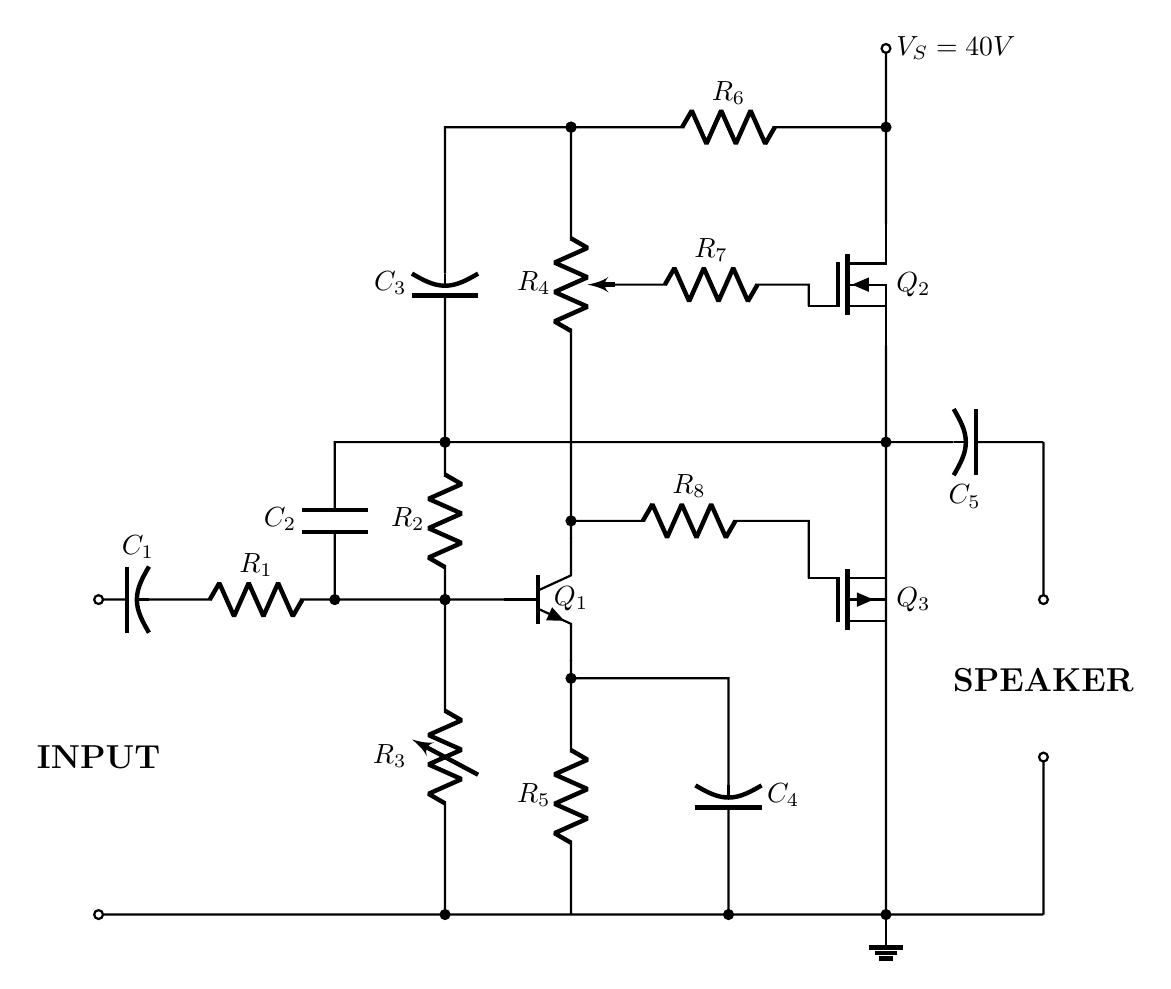
\begin{tikzpicture}[scale=2]
  \draw[color=black, thick]
    (0,0) to [short,o-] (6,0){} % Baseline for connection to ground
    % Input and ground
    (0,1) node[]{\large{\textbf{INPUT}}}
    % Connection of passive components
    (5,0) node[ground]{} node[circ](4.5,0){}
    (0,2) to [cC, l=$C_1$, o-] (0.5,2)
    to [R,l=$R_1$,](1.5,2)
    to node[short]{}(2.6,2)
    (1.5,2) to [C, l=$C_2$, *-] (1.5,3) -| (5,3)
    (2.2,2) to [R, l=$R_2$, *-*] (2.2,3)
    (2.2,3) to [cC, l=$C_3$, *-] (2.2,5) -| (3,5)
    % Transistor Bipolar Q1
    (3,0) to [R,l=$R_5$,-*] (3,1.5)
    to [Tnpn,n=npn1] (3,2.5)
    (npn1.E) node[right=3mm, above=5mm]{$Q_1$} % Labelling the NPN transistor
    (4,0) to [cC, l_=$C_4$, *-] (4, 1.5)--(3,1.5)
    (2.2,0) to [vR, l=$R_3$, *-*] (2.2,2)
    (3,2.5) to node[short]{}(3,3)
    (3,5) to [pR, n=pot1, l_=$R_4$, *-] (3,3)
    (3,5) to [R, l=$R_6$, *-] (5,5)
    to [short,*-o](5,5.5) node[right]{$V_S=40 V$}
    % Mosfet Transistors
    (5,3) to [Tnigfetd,n=mos1] (5,5)
    (mos1.B) node[anchor=west]{$Q_2$} % Labelling MOSFET Q2 Transistor
    (pot1.wiper) to [R, l=$R_7$] (4.5,4) -| (mos1.G)
    (5,1.5) to [Tpigfetd,n=mos2] (5,2.5)
    (5,0) to (mos2.S)
    (3,2.5) to [R, l=$R_8$, *-] (4.5,2.5)
    -| (mos2.G)
    (mos2.B) node[anchor=west]{$Q_3$} % Labelling MOSFET Q3 Transistor
    % Output
    (6,3) to [cC, l=$C_5$,-*](5,3)
    (6,3) to [short,-o] (6,2){}
    (mos1.S)--(mos2.D)
    (6,0) to [short,-o] (6,1){} node[above=7mm]{\large{\textbf{SPEAKER}}}
    ;
\end{tikzpicture}
\end{VerbatimOut}

\MyIO


\begin{VerbatimOut}{z.out}


\section{Kalman Filter System Model}

This Kalman filter system model was done by Burkart Lingner
\cite{lingner2010}.
\ix{Lingner, Burkart}

% An example using TikZ/PGF 2.00
%
% Features: Decorations, Fit, Layers, Matrices, Styles
% Tags: Block diagrams, Diagrams
% Technical area: Electrical engineering

%%%% \documentclass[a4paper,10pt]{article}
%%%% 
%%%% \usepackage[english]{babel}
%%%% \usepackage[T1]{fontenc}
%%%% \usepackage[ansinew]{inputenc}
%%%% 
%%%% \usepackage{lmodern}	% font definition
%%%% \usepackage{amsmath}	% math fonts
%%%% \usepackage{amsthm}
%%%% \usepackage{amsfonts}
%%%% 
%%%% \usepackage{tikz}
%%%% 
%%%% %%%<
%%%% \usepackage{verbatim}
%%%% \usepackage[active,tightpage]{preview}
%%%% \PreviewEnvironment{tikzpicture}
%%%% \setlength\PreviewBorder{5pt}%
%%%% %%%>
%%%% 
%%%% \begin{comment}
%%%% :Title: Kalman Filter System Model
%%%% :Slug: kalman-filter
%%%% :Author: Burkart Lingner
%%%% 
%%%% This is the system model of the (linear) Kalman filter. 
%%%% 
%%%% \end{comment}
%%%% 
%%%% 

\begin{figure}[htbp]
\caption{Kalman filter system model}
\centering
% The state vector is represented by a blue circle.
% "minimum size" makes sure all circles have the same size
% independently of their contents.
\tikzstyle{state}=[circle,
                                    thick,
                                    minimum size=1.2cm,
                                    draw=blue!80,
                                    fill=blue!20]

% The measurement vector is represented by an orange circle.
\tikzstyle{measurement}=[circle,
                                                thick,
                                                minimum size=1.2cm,
                                                draw=orange!80,
                                                fill=orange!25]

% The control input vector is represented by a purple circle.
\tikzstyle{input}=[circle,
                                    thick,
                                    minimum size=1.2cm,
                                    draw=purple!80,
                                    fill=purple!20]

% The input, state transition, and measurement matrices
% are represented by gray squares.
% They have a smaller minimal size for aesthetic reasons.
\tikzstyle{matrx}=[rectangle,
                                    thick,
                                    minimum size=1cm,
                                    draw=gray!80,
                                    fill=gray!20]

% The system and measurement noise are represented by yellow
% circles with a "noisy" uneven circumference.
% This requires the TikZ library "decorations.pathmorphing".
\tikzstyle{noise}=[circle,
                                    thick,
                                    minimum size=1.2cm,
                                    draw=yellow!85!black,
                                    fill=yellow!40,
                                    decorate,
                                    decoration={random steps,
                                                            segment length=2pt,
                                                            amplitude=2pt}]

% Everything is drawn on underlying gray rectangles with
% rounded corners.
\tikzstyle{background}=[rectangle,
                                                fill=gray!10,
                                                inner sep=0.2cm,
                                                rounded corners=5mm]

\begin{tikzpicture}[>=latex,text height=1.5ex,text depth=0.25ex]
    % "text height" and "text depth" are required to vertically
    % align the labels with and without indices.
  
  % The various elements are conveniently placed using a matrix:
  \matrix[row sep=0.5cm,column sep=0.5cm] {
    % First line: Control input
    &
        \node (u_k-1) [input]{$\mathbf{u}_{k-1}$}; &
        &
        \node (u_k)   [input]{$\mathbf{u}_k$};     &
        &
        \node (u_k+1) [input]{$\mathbf{u}_{k+1}$}; &
        \\
        % Second line: System noise & input matrix
        \node (w_k-1) [noise] {$\mathbf{w}_{k-1}$}; &
        \node (B_k-1) [matrx] {$\mathbf{B}$};       &
        \node (w_k)   [noise] {$\mathbf{w}_k$};     &
        \node (B_k)   [matrx] {$\mathbf{B}$};       &
        \node (w_k+1) [noise] {$\mathbf{w}_{k+1}$}; &
        \node (B_k+1) [matrx] {$\mathbf{B}$};       &
        \\
        % Third line: State & state transition matrix
        \node (A_k-2)         {$\cdots$};           &
        \node (x_k-1) [state] {$\mathbf{x}_{k-1}$}; &
        \node (A_k-1) [matrx] {$\mathbf{A}$};       &
        \node (x_k)   [state] {$\mathbf{x}_k$};     &
        \node (A_k)   [matrx] {$\mathbf{A}$};       &
        \node (x_k+1) [state] {$\mathbf{x}_{k+1}$}; &
        \node (A_k+1)         {$\cdots$};           \\
        % Fourth line: Measurement noise & measurement matrix
        \node (v_k-1) [noise] {$\mathbf{v}_{k-1}$}; &
        \node (H_k-1) [matrx] {$\mathbf{H}$};       &
        \node (v_k)   [noise] {$\mathbf{v}_k$};     &
        \node (H_k)   [matrx] {$\mathbf{H}$};       &
        \node (v_k+1) [noise] {$\mathbf{v}_{k+1}$}; &
        \node (H_k+1) [matrx] {$\mathbf{H}$};       &
        \\
        % Fifth line: Measurement
        &
        \node (z_k-1) [measurement] {$\mathbf{z}_{k-1}$}; &
        &
        \node (z_k)   [measurement] {$\mathbf{z}_k$};     &
        &
        \node (z_k+1) [measurement] {$\mathbf{z}_{k+1}$}; &
        \\
    };
    
    % The diagram elements are now connected through arrows:
    \path[->]
        (A_k-2) edge[thick] (x_k-1)	% The main path between the
        (x_k-1) edge[thick] (A_k-1)	% states via the state
        (A_k-1) edge[thick] (x_k)		% transition matrices is
        (x_k)   edge[thick] (A_k)		% accentuated.
        (A_k)   edge[thick] (x_k+1)	% x -> A -> x -> A -> ...
        (x_k+1) edge[thick] (A_k+1)
        
        (x_k-1) edge (H_k-1)				% Output path x -> H -> z
        (H_k-1) edge (z_k-1)
        (x_k)   edge (H_k)
        (H_k)   edge (z_k)
        (x_k+1) edge (H_k+1)
        (H_k+1) edge (z_k+1)
        
        (v_k-1) edge (z_k-1)				% Output noise v -> z
        (v_k)   edge (z_k)
        (v_k+1) edge (z_k+1)
        
        (w_k-1) edge (x_k-1)				% System noise w -> x
        (w_k)   edge (x_k)
        (w_k+1) edge (x_k+1)
        
        (u_k-1) edge (B_k-1)				% Input path u -> B -> x
        (B_k-1) edge (x_k-1)
        (u_k)   edge (B_k)
        (B_k)   edge (x_k)
        (u_k+1) edge (B_k+1)
        (B_k+1) edge (x_k+1)
        ;
    
    % Now that the diagram has been drawn, background rectangles
    % can be fitted to its elements. This requires the TikZ
    % libraries "fit" and "background".
    % Control input and measurement are labeled. These labels have
    % not been translated to English as "Measurement" instead of
    % "Messung" would not look good due to it being too long a word.
    \begin{pgfonlayer}{background}
        \node [background,
                    fit=(u_k-1) (u_k+1),
                    label=left:Entrance:] {};
        \node [background,
                    fit=(w_k-1) (v_k-1) (A_k+1)] {};
        \node [background,
                    fit=(z_k-1) (z_k+1),
                    label=left:Measure:] {};
    \end{pgfonlayer}
\end{tikzpicture}

\end{figure}
\end{VerbatimOut}

\MyIO


% Linguistics.
\ProvidesFile{ap-linguistics.tex}[2022-05-16 linguistics appendix]

\begin{VerbatimOut}{z.out}
\chapter{LINGUISTICS}
\ix{linguistics//Linguistics appendix}

See WIKIBOOKS \LaTeX/Linguistics \cite{wikibooks-latex-linguistics}
or google for the information you need.

The doulossil font
\cite{tambe2020}
is a TrueType font.
Version 0.1 on September 21, 2020 claimed
``it has characters that are not in other TeX IPA fonts''.
\end{VerbatimOut}

\MyIO


\begin{VerbatimOut}{z.out}


\section{Demonstrate the example and examples environments}

The example and examples environment
are defined
in the covington
\cite{covington2021}
package.

Demonstrate the example environment:
\begin{example}
  This is an example.
  This is an example.
\end{example}

Demonstrate the examples environment:
\begin{examples}
  \item First example.
  \item Second example.
\end{examples}
\end{VerbatimOut}

\MyIO


  


% Mathematics.
\ProvidesFile{ap-mathematics.tex}[2022-07-13 mathematics appendix]

\begin{VerbatimOut}{z.out}
\chapter{MATHEMATICS}
\ix{mathematics//Mathematics appendix}

\PurdueThesisLogo\ loads the \AMSmathLogo\ package
\cite{amslatex3project2019}
to do mathematics.
\end{VerbatimOut}

\MyIO




\begin{VerbatimOut}{z.out}

International standard ISO 80000-2:2019
\cite{iso8000022019}
states that \(\mit e\),~%
\(\mit i\),~%
\(\mit j\),~%
and \(\itpi\) should appear as
\(\mathup e\),~%
\(\mathup i\),~%
\(\mathup j\),~%
and~\(\mathup \pi\) because they are constants.
I had thesis.tex set up to do this automatically
and got complaints that i was not in a math italic font.
By default I'm now setting things up so e and pi
are set in an upright font automatically
and i and j are set in a math italic font.
So the new defaults, when typset in math mode, are
\begin{inlinetable}
  \begin{tabular}{@{}lllllllll@{}}
    \textbf{Description}&
      \textbf{In}& \textbf{Out}\qquad& \textbf{In}& \textbf{Out}\qquad&
      \textbf{In}& \textbf{Out}& \textbf{In}& \textbf{Out}\\
    \midrule
    New Default&               |e|&   \(e\)&    |i|&  \(i\)&  |j|&  \(j\)&  |\pi|&   \(\pi\)\\
    To Get Other Symbol\qquad& |\ite|& \(\ite\)\quad& |\i|& \(\i\)\quad& |\j|& \(\j\)\quad& |\itpi|& \(\itpi\)\\
    \bottomrule
  \end{tabular}
\end{inlinetable}
\end{VerbatimOut}

\MyIO


\begin{VerbatimOut}{z.out}
  
Euler's identity is
\begin{equation*}
  e^{\i\pi} + 1 = 0.
\end{equation*}
\end{VerbatimOut}

\MyIO


\begin{VerbatimOut}{z.out}

Here's a simple formula relating $e$,~$i$,~$\pi$, and~$\phi$,
the golden ratio
\begin{equation}
  e^{\i\pi} + 2\phi = \sqrt 5.
\end{equation}
I didn't notice anything on the web about putting the symbol for
the golden ratio in a special font even though it is a constant.
\end{VerbatimOut}

\MyIO


\begin{VerbatimOut}{z.out}
There are two types of mathematics in \LuaLaTeXLogo.
Text math is math that that is interspersed with text.
For example, \(a = b + c\), is text math.
Display math is math that is away from the text on
line(s) of it's own.
For example,
\begin{equation}
  a = b + c
\end{equation}
\end{VerbatimOut}

\MyIO


\begin{VerbatimOut}{z.out}
\newpage

\section{Standard Functions}

Standard functions should be in a roman font.
Like this: \(\cos\theta\).
Here is a list of standard function commands:

\begin{inlinetable}
  \begin{tabular}{@{}llll@{}}
    \verb+\arccos+& \verb+\csc+& \verb+\ker+&    \verb+\min+\\
    \verb+\arcsin+& \verb+\deg+& \verb+\lg+&     \verb+\Pr+\\
    \verb+\arctan+& \verb+\det+& \verb+\lim+&    \verb+\sec+\\
    \verb+\arg+&    \verb+\dim+& \verb+\liminf+& \verb+\sin+\\
    \verb+\cos+&    \verb+\exp+& \verb+\limsup+& \verb+\sinh+\\
    \verb+\cosh+&   \verb+\gcd+& \verb+\ln+&     \verb+\sup+\\
    \verb+\cot+&    \verb+\hom+& \verb+\log+&    \verb+\tan+\\
    \verb+\coth+&   \verb+\inf+& \verb+\max+&    \verb+\tanh+\\
  \end{tabular}
  \ix
  {%
    arccos//arcsin//arctan//arg//cos//cosh//cot//coth%
    //csc//deg//det//dim//exp//gcd//hom//inf%
    //ker//lg//lim//liminf//limsup//ln//log//max%
    //min//Pr//sec//sin//sinh//sup//tan//tanh%
  }
  \index{\verb+\arccos+} \index{\verb+\arcsin+} \index{\verb+\arctan+} \index{\verb+\arg+}
  \index{\verb+\cos+} \index{\verb+\cosh+} \index{\verb+\cot+} \index{\verb+\coth+}
  \index{\verb+\csc+} \index{\verb+\deg+} \index{\verb+\det+} \index{\verb+\dim+}
  \index{\verb+\exp+} \index{\verb+\gcd+} \index{\verb+\hom+} \index{\verb+\inf+}
  \index{\verb+\ker+} \index{\verb+\lg+} \index{\verb+\lim+} \index{\verb+\liminf+}
  \index{\verb+\limsup+} \index{\verb+\ln+} \index{\verb+\log+} \index{\verb+\max+}
  \index{\verb+\min+} \index{\verb+\Pr+} \index{\verb+\sec+} \index{\verb+\sin+}
  \index{\verb+\sinh+} \index{\verb+\sup+} \index{\verb+\tan+} \index{\verb+\tanh+}
\end{inlinetable}
\end{VerbatimOut}

\MyIO


\begin{VerbatimOut}{z.out}
\newpage

\section{English Words in Math}

English words in math should be in a roman font like this:\\
Let the maximum value of \(a\) be \(a_\text{max}\).\\
\(a_\text{max} \ge a_\text{min}\) should always be true.\\
The temperature in the attic is \(t_\text{attic}\).
\end{VerbatimOut}

\MyIO


\begin{VerbatimOut}{z.out}
\section{Text Math}

Use |\(| to start text math
and |\)| to end text math.
Some people use |$| to start and end text math---I
don't recommend that because \LaTeX\
can give better error messages
if you use |\(|
and |\)|.
\end{VerbatimOut}

\MyIO


\begin{VerbatimOut}{z.out}
\section{Displayed Equations}

Do not use \verb+$$+ to start or end displayed math like \TeX\ uses
\cite{gratzer2016}.

The \AMSmathLogo\ package provides a number
of additional displayed equation structures
beyond the ones provided in basic \LaTeX.
The augmented set includes
\cite{amslatex3project2019b}:

\begin{inlinetable}
  \begin{tabular}{@{}ll@{}}
    \toprule
    \textbf{Environment}& \textbf{Used for}\\
    \midrule
    \tt equation& used for single equations\\
    \tt multline& split single equations over multiple lines\\
    \tt gather& collect but do not align multiple equations\\
    \tt align& align multiple equations\\
    \tt alignat& aligns multiple equations at multiple places\\
    \tt flalign& aligns multiple equations at multiple places on full length lines\\
    \tt split& split a single equation over multiple lines\\
    \bottomrule
  \end{tabular}
\end{inlinetable}

All but \verb+split+ can be followed by \verb+*+ to not number equations.
\end{VerbatimOut}

\MyIO


\begin{VerbatimOut}{z.out}

\subsection{\texttt{equation} environment}

The \verb+equation+ environment is used for single equations.

\begin{equation}
  E = mc^2
\end{equation}
\end{VerbatimOut}

\MyIO


\begin{VerbatimOut}{z.out}

The \verb+equation*+ environment does single, unnumbered equations.

\begin{equation*}
  a = b_0c + \frac12 de^2 + {\textstyle \frac12} fg^2
    + h_1 + h_2 + \cdots + h_n
    \qquad \text{for \(c \ne d\) and \(g < \infty\)}
\end{equation*}
\end{VerbatimOut}

\MyIO


\begin{VerbatimOut}{z.out}

\textcite{greene-2021-03-14}
wrote
\begin{quote}
  For
  \href{https://twitter.com/hashtag/PiDay?src=hashtag\_click\#PiDay}{\#PiDay},
  one of the coolest formulae for today's honoree:
  \[
    \frac 1\pi
    =
    \frac {\sqrt8} {9801}
    \sum_{n=0}^\infty
    \frac  {(4n!) (1103+26390n)}  {(n!)^4 396^{4n}}
  \]
\end{quote}
\end{VerbatimOut}

\MyIO


\begin{VerbatimOut}{z.out}

International standard ISO 80000-2:2019
\cite{iso8000022019}
states that the ``$d\/$'' in math differentials
should be typeset as ``$\di$''.
So,
\begin{equation*}
  \text{use } \int x\di x\qquad\qquad \text{instead of } \int x\,dx
\end{equation*}
\end{VerbatimOut}

\MyIO


\begin{VerbatimOut}{z.out}

The formula for Bekenstein-Hawking entropy:

\begin{equation*}
  S_\text{BH}
  =
  \frac A {4L_P^2}
  = \frac {c^3A} {4G\hbar}
\end{equation*}
\end{VerbatimOut}

\MyIO


\begin{VerbatimOut}{z.out}

Type in the math and let \LaTeX\ worry about the spacing.
You only need to do fine tuning by hand if it looks bad.

Another \verb+equation*+ environment,
note the spacing before the large close parenthesis:

\begin{equation*}
  \frac ab
    = ab^{-1}
    % Parens are the wrong size.
    = (\sqrt{\frac ab})^2
    % Parens are the right size but closing paren is too close to radical.
    = \left( \sqrt\frac ab \right)^2
    % Parens are right size but a negative thin space puts closing paren on top of radical.
    = \left( \sqrt\frac ab \!\right)^2
    % Parens are right size but a thin space puts closing paren too close to radical.
    = \left( \sqrt\frac ab \,\right)^2
    % Parens are right size but a medium space puts closing paren too close to radical.
    = \left( \sqrt\frac ab \:\right)^2
    % Parens are right size and I think a thick space looks the best.
    = \left( \sqrt\frac ab \;\right)^2
\end{equation*}
\end{VerbatimOut}

\MyIO


\begin{VerbatimOut}{z.out}

\begin{equation*}
  (\cos x)^2 + (\sin x)^2 = \cos^2 x + \sin^2 x = 1
\end{equation*}
\end{VerbatimOut}

\MyIO


\begin{VerbatimOut}{z.out}

\begin{equation}
  x \mod 2 =
  \begin{cases}
    0& \text{if $x$ is even}\\
    1& \text{if $x$ is odd}\\
  \end{cases}
\end{equation}
\end{VerbatimOut}

\MyIO


\begin{VerbatimOut}{z.out}

The first six derivatives of distance are velocity, acceleration, jerk, snap, crackle,
and pop
\cite{reid2013}.

\begin{equation}
  % Every array element should be in \displaystyle (a big font).
  \AtBeginEnvironment{array}{\everymath{\displaystyle}}
  % Set space between columns to zero, use {} = ... to add a little space before the = "by hand".
  \arraycolsep = 0pt
  \text{distance derivitives} = \left\{\ %
    \begin{array}{llllllll}
      % I'm formatting the first 4 lines different from the last 3 so this will fit on one page.
      x&      {}=\text{distance}&     {}=vt\\[2pt]
      v&      {}=\text{velocity}&     {}=\frac{\di x}{\di t}\\[9pt]
      a&      {}=\text{acceleration}& {}=\frac{\di v}{\di t}& {}=\frac{\di^2x}{\di t^2}\\[9pt]
      \mit j& {}=\text{jerk}&         {}=\frac{\di a}{\di t}& {}=\frac{\di^2v}{\di t^2}&
        {}=\frac{\di^3x}{\di t^3}\\[9pt]
      s
        & {}=\text{snap}
        & {}=\frac{\di \mit j}{\di t}
        & {}=\frac{\di^2a}{\di t^2}
        & {}=\frac{\di^3v}{\di t^3}
        & {}=\frac{\di^4x}{\di t^4}\\[9pt]
      c
        & {}=\text{crackle}
        & {}=\frac{\di s}{\di t}
        & {}=\frac{\di^2\mit j}{\di t^2}
        & {}=\frac{\di^3a}{\di t^3}
        & {}=\frac{\di^4v}{\di t^4}
        & {}=\frac{\di^5x}{\di t^5}\\[9pt]
      p
        & {}=\text{pop}
        & {}=\frac{\di c}{\di t}
        & {}=\frac{\di^2s}{\di t^2}
        & {}=\frac{\di^3\mit j}{\di t^3}
        & {}=\frac{\di^4a}{\di t^4}
        & {}=\frac{\di^5v}{\di t^5}
        & {}=\frac{\di^6x}{\di t^6}
    \end{array}
  \right.
\end{equation}
\end{VerbatimOut}

\MyIO


\begin{VerbatimOut}{z.out}

\subsection{\texttt{multline} environment}

The \verb+multline+ environment is used
to split single equations over multiple lines.

\begin{multline}
  S = a + b + c + d + e + f + g + h + i + j\\
  + k + l + m + n + o + p\\
  + q + r + s + t + u + v + w + x + y + z
\end{multline}
\end{VerbatimOut}

\MyIO


\begin{VerbatimOut}{z.out}

\begin{multline}
  S = a + b + c + d + e\\
  + f + g + h + i + j\\
  + k + l + m + n + o\\
  + p + q + r + s + t\\
  + u + v + w + x + y\\
  + z
\end{multline}
\end{VerbatimOut}

\MyIO


\begin{VerbatimOut}{z.out}

% Calculate width of space before equation plus equation number.
% (All digits are the same width.)
\newdimen{\tdimen}
\settowidth{\tdimen}{\kern\multlinetaggap (L.5)}
\begin{multline}
  S = a + b + c + d + e\\
  \makebox[\textwidth]{\hfill $+ f + g + h + i + j$\hfill\hfill\hfill\hfill\kern\tdimen}\\
  \makebox[\textwidth]{\hfill\hfill${} + k + l + m + n + o$\hfill\hfill\hfill\kern\tdimen}\\
  \makebox[\textwidth]{\hfill\hfill\hfill${} + p + q + r + s + t$\hfill\hfill\kern\tdimen}\\
  \makebox[\textwidth]{\hfill\hfill\hfill\hfill${} + u + v + w + x + y$\hfill\kern\tdimen}\\
  + z
\end{multline}
\end{VerbatimOut}

\MyIO


\begin{VerbatimOut}{z.out}

\subsection{\texttt{gather} environment}

The \verb+gather+ environment collects but does not align multiple equations.

\begin{gather}
  a = b + c + d + e + f + g + h + i + j + k + l\\
  m = n + o + p + q + r + s + t + u + v + w + x + y + z
\end{gather}
\end{VerbatimOut}

\MyIO


\begin{VerbatimOut}{z.out}

\begin{gather}
  a = b + c + d + e + f + g + h + i + j + k + l\notag\\
  m = n + o + p + q + r + s + t + u + v + w + x + y + z
\end{gather}
\end{VerbatimOut}

\MyIO


\begin{VerbatimOut}{z.out}

\begin{gather*}
  \alpha = \beta + \gamma + \delta + \eta\\
  \theta = \iota + \kappa + \lambda + \mu + \nu + \rho + \tau
\end{gather*}
\end{VerbatimOut}

\MyIO


\begin{VerbatimOut}{z.out}

\begin{gather}
  x_\text{min} + x_\text{max} \le \sum_{i=1}^n x_i\\
  x_\text{min} + x_\text{max}
    = \sum_{i=1}^n x_i - \sum_{i=2}^{n-1} x_i\quad\text{if $x$ is sorted}\\
  x_\text{min} \le \left(\sum_{i=1}^n x_i\right) / n
\end{gather}
\end{VerbatimOut}

\MyIO


\begin{VerbatimOut}{z.out}

\subsection{\texttt{align} environment}

The \verb+align+ environment aligns multiple equations.

\begin{align}
  a &= b + c + d\\
  e &= f + g + h + i + j
\end{align}
\end{VerbatimOut}

\MyIO


\begin{VerbatimOut}{z.out}

\begin{align}
  x = \frac{-b \pm \sqrt{b^2-4ac}}{2a}\notag\\
  % Put a thin space before the b^2 to improve the appearance.
  x = \frac{-b \pm \sqrt{\,b^2-4ac}}{2a}
\end{align}
\end{VerbatimOut}
\ix{align environment}
\index{\verb+\begin{align}+}
\ix{thin space}
\index{\verb+\,+}

\MyIO


\begin{VerbatimOut}{z.out}

Quadratic formula proof
\cite{khan2018}:
\ix{quadratic formula}

% The align environment requires the amsmath package.
% Use \addtolength{\jot}{6pt} to increase the space between rows in an amsmath multi-line math formula.
% That's not done here so everything will fit on one page.
\begin{align}
  ax^2 + bx + c &= 0\\
  ax^2 + bx &= -c\notag\\
  % The "\," adds a thinspace of horizontal space.
  x^2 + \frac ba\,x &= -\frac ca\notag\\
  x^2 + \frac ba\,x + \frac{b^2}{4a^2} &= \frac{b^2}{4a^2} - \frac ca\notag\\
  \left(x + \frac b{2a}\right)^2 &= \frac{b^2}{4a^2} - \frac ca\notag\\
  \left(x + \frac b{2a}\right)^2 &= \frac{b^2}{4a^2} - \frac{4ac}{4a^2}\notag\\
  \left(x + \frac b{2a}\right)^2 &= \frac{b^2-4ac}{4a^2}\notag\\
  \sqrt{\left(x + \frac b{2a}\right)^2}
    &= \sqrt{\left(\frac{b^2-4ac}{4a^2}\right)}\notag\\
  x + \frac b{2a} &= \pm \frac{\sqrt{\,b^2-4ac}}{\sqrt{4a^2}}\notag\\
  x + \frac b{2a} &= \pm \frac{\sqrt{\,b^2-4ac}}{2a}\notag\\
  x &= - \frac b{2a} \pm \frac{\sqrt{\,b^2-4ac}}{2a}\notag\\
  x &= \frac{-b \pm \sqrt{\,b^2-4ac}}{2a}
\end{align}
\end{VerbatimOut}

\MyIO


\begin{VerbatimOut}{z.out}

\subsection{\texttt{alignat} environment}
\index{\verb+\begin{aligo}+@\verb+\begin{alignat}+}
\ix{alignat environment}

The \verb+alignat+ environment aligns multiple equations at multiple places.
\begin{alignat}{2}
  a &= b& \qquad\qquad& \text{set $a$}\\
  c &= d& &             \text{you guessed it, set $c$}\notag\\
  g &= h& &             \text{and finally, set $g$}
\end{alignat}
\index{\verb+\begin{aligo}+@\verb+\begin{alignat}+}
\ix{alignat environment}

I like to align input columns on the input if possible
and will sometimes use windows over~250 characters wide to do so.
If that won't work I sometimes do,
for example,
\begin{alignat}{2}
  a
    &= b
    & \qquad\qquad
    & \text{set $a$}\\
  c
    &= d
    &
    &\text{you guessed it, set $c$}\notag\\
  g
    &= h
    &
    &\text{and finally, set $g$}
\end{alignat}
\index{\verb+\begin{aligo}+@\verb+\begin{alignat}+}
\ix{alignat environment}

Do whatever works best for you.

\end{VerbatimOut}

\MyIO


\begin{VerbatimOut}{z.out}

Quadratic formula proof
\cite{khan2018}:

% Make changes to \jot be local to the group that starts on the next line.
{
  % Increase distance between lines by 6pt.
  \addtolength{\jot}{6pt}
  \begin{alignat}{2}
    ax^2 + bx + c
      &= 0
      &
      &\text{subtract $c$}\\
    ax^2 + bx
      &= -c
      &
      &\text{divide by $a$}\notag\\
    % The "\," adds a thinspace of horizontal space.
    x^2 + \frac ba\,x
      &= -\frac ca
      &
      &\text{add $\displaystyle\frac{b^2}{4a^2}$}\notag\\
    x^2+\frac ba\,x+\frac{b^2}{4a^2}
      &= \frac{b^2}{4a^2}-\frac ca
      &
      &\text{factor left hand side}\notag\\
    \left(x+\frac b{2a}\right)^2
      &= \frac{b^2}{4a^2}-\frac ca
      &
      &\text{multiply right-most term by $\displaystyle\frac{4a}{4a}$}\notag\\
    \left(x + \frac b{2a}\right)^2
      &= \frac{b^2}{4a^2}-\frac{4ac}{4a^2}
      &
      &\text{use common denominator}\notag\\
    \left(x + \frac b{2a}\right)^2
      &= \frac{b^2-4ac}{4a^2}
      &
      &\text{take square root of each side}\notag\\
    \sqrt{\left(x + \frac b{2a}\right)^2}
      &= \sqrt{\left(\frac{b^2-4ac}{4a^2}\right)}
      &
      &\text{compute square root of each side}\notag\\
    x + \frac b{2a}
      &= \pm \frac{\sqrt{\,b^2-4ac}}{\sqrt{4a^2}}
      &
      &\text{simplify right hand denominator}\notag\\
    x + \frac b{2a}
      &= \pm \frac{\sqrt{\,b^2-4ac}}{2a}
      &
      &\text{subtract $\displaystyle\frac b{2a}$ from each side}\notag\\
    x
      &= -\frac b{2a} \pm \frac{\sqrt{\,b^2-4ac}}{2a}
      &\qquad
      &\text{use common denominator}\notag\\
    x
      &= \frac{-b \pm \sqrt{\,b^2-4ac}}{2a}
  \end{alignat}
}
\end{VerbatimOut}

\MyIO


\begin{VerbatimOut}{z.out}

\index{\verb+\begin{flalign}+}
\todoindex{Verb+Begin-Ocurly-flalign-Ccurly+}
\ix{falign environment}
\subsection{\texttt{flalign} environment}

The \verb+flalign+ environment aligns multiple equations at multiple places
on full length lines.

\begin{flalign}
  a &= b&   &   & u &= v\\
  c &= d& m &= n& w &= x\notag\\
  g &= h&   &   & y &= z
\end{flalign}
\end{VerbatimOut}

\MyIO


\begin{VerbatimOut}{z.out}

\index{\verb+\begin{split}+}
\todoindex{Verb+Begin-Ocurly-split-Ccurly+}
\ix{split environment}
\subsection{\texttt{split} environment}

The \verb+split+ environment ???.
\end{VerbatimOut}

\MyIO
\index{\verb+\begin{split}+}
\todoindex{Verb+Begin-Ocurly-split-Ccurly+}
\ix{split environment}


\begin{VerbatimOut}{z.out}
\section{Theorem-like environments}

These theorem-like environments are defined
in the amsthm package or in\\  % break line here so we don't go past right margin
\verb+PurdueThesis.cls+.
\end{VerbatimOut}

\MyIO


\begin{VerbatimOut}{z.out}

\index{\verb+\begin{definition}+}
\todoindex{Verb+Begin-Ocurly-definition-Ccurly+}
\ix{definition environment}
\begin{definition}
  This is an example definition.
  This is an example definition.
  This is an example definition.
  This is an example definition.
  This is an example definition.
\end{definition}

\index{\verb+\begin{observation}+}
\todoindex{Verb+Begin-Ocurly-observation-Ccurly+}
\ix{observation environment}
\begin{observation}
  This is an example observation.
  This is an example observation.
  This is an example observation.
  This is an example observation.
  This is an example observation.
\end{observation}

\index{\verb+\begin{proof}+}
\todoindex{Verb+Begin-Ocurly-proof-Ccurly+}
\ix{proof environment}
\begin{proof}
  This is an example proof.
  This is an example proof.
  This is an example proof.
  This is an example proof.
  If \(a = b\) and \(b = c\) then \(a = c\).
\end{proof}

\index{\verb+\begin{proposition}+}
\todoindex{Verb+Begin-Ocurly-proposition-Ccurly+}
\ix{proposition environment}
\begin{proposition}
  This is an example proposition.
  This is an example proposition.
  This is an example proposition.
  This is an example proposition.
  This is an example proposition.
\end{proposition}

\index{\verb+\begin{theorem}+}
\todoindex{Verb+Begin-Ocurly-theorem-Ccurly+}
\ix{theorem environment}
\begin{theorem}
  This is an example theorem.
  This is an example theorem.
  This is an example theorem.
  This is an example theorem.
  This is an example theorem.
\end{theorem}
\end{VerbatimOut}

\MyIO


\begin{VerbatimOut}{z.out}


\section{Examples}

\subsection{Bayes' Theorem}
\ix{Bayes' Theorem}

Bayes' Theorem
\cite{bayes}:

{
  \UndefineShortVerb{\|}
\[
  \text{P}(\text A|\text B)
    % The "\," puts a thin horizontal space there, 1/6 of an "em".
    % An "em" is roughly the width of a lowercase "m".
    = \frac{\text P(\text B|\text A)\,\text P(\text A)}{\text P(\text B)}
\]
}
\end{VerbatimOut}

\MyIO


\begin{VerbatimOut}{z.out}

\subsection{Nicomachus's theorem}
\ix{Nicomachus's theorem}

Nicomachus's theorem
\cite{wikipedia-nicomachus}
states that
the sum of the first~\(n\) cubes is the square of the~\(n\)th triangular number.
That is,
\[
  1^3 + 2^3 + 3^3 + \cdots + n^3 = (1 + 2 + 3 + \cdots + n)^2.
\]
The same equation may be written more compactly using the mathematical notation for summation:
\[
  \sum_{k=1}^n k^3 = \left(\sum_{k=1}^n k\right)^2.
\]
Also see the diagram on that web page.
\end{VerbatimOut}

\MyIO


\begin{VerbatimOut}{z.out}

\subsection{Prime Number Theorem}
\ix{Prime Number Theorem}

\textcite{li2013}
suggested using a functional equation
from the Prime Number Theorem proof
as an example:
\begin{equation}
  \int_1^x
    \sum_{p\le u}
    \left\lfloor\frac{\log u}{\log p}\right\rfloor
    \log p
    \,\text{d}u
    =
    \frac1{2\pi i}
    \int_{c-i\infty}^{c+i\infty}
    \frac{x^{s+1}}{s(s+1)}
    \left(-\frac{\zeta'(s)}{\zeta(s)}\right)
    \text{d}s
\end{equation}
\end{VerbatimOut}

\MyIO


\begin{VerbatimOut}{z.out}

\subsection{Quantum Mechanics}
\ix{Quantum Mechanics}

\textcite{greene-2021-04-04}
wrote
\ix{Greene, Brian Randolph}
\begin{quotation}
  Quantum Mechanics in a nutshell:
  A particle goes from here to there
  by sampling every possible trajectory from here to there.

  \[
    \langle x_f,t_f \vert x,t_{\mathit i} \rangle
    =
    \sum_{\text p \in \text{paths}} e^{\mathit iS(\text p) \si{\planckbar}}
  \]
\end{quotation}
\end{VerbatimOut}

\MyIO


%  https://tex.stackexchange.com/questions/96568/how-can-i-align-multiple-cases-environment-simultaneously
\begin{VerbatimOut}{z.out}
\subsection{Question in String Theory / Mass of States / Number Operator}


\textcite{yourlazyphysicist2017}
wrote
``I have the following definition of the space-time coordinates'':

\newcommand{\fpt}{{4\pi T}}
\newcommand{\oh}{\frac12}
\newcommand{\snnz}{\sum_{n\ne0}}
\newcommand{\tms}{\tau - \sigma}
\newcommand{\tps}{\tau + \sigma}
\begin{align}
    \text{closed string: }&
        \begin{cases}
            \displaystyle
            X^\mu_R
                = \oh x^\mu
                + \frac1\fpt (\tms) p^\mu
                + \frac i{\sqrt\fpt} \snnz \frac1n \alpha^\mu_n e^{-in(\tms)},\\
            \displaystyle
            X^\mu_L
                = \oh x^\mu
                + \frac1\fpt (\tps) p^\mu
                + \frac i{\sqrt\fpt} \snnz \frac1n \tilde\alpha^\mu_n e^{-in(\tps)}.
        \end{cases}\\[6pt]
    \text{open string: }&
        \begin{cases}
            \displaystyle
            X^\mu_N
                = x^\mu
                + \frac1{\pi T}p^\mu\tau
                + \frac i{\sqrt{\pi T}} \snnz \frac1n \alpha^\mu_n e^{-in\tau} \cos(n\sigma),\\
            \displaystyle
            X^\mu_D
                = x^\mu
                + \frac i{\sqrt{\pi T}} \snnz \frac1n \alpha^\mu_n e^{-in\tau} \sin(n\sigma).
        \end{cases}
\end{align}
\end{VerbatimOut}

\MyIO



% https://www.google.com/url?sa=i&rct=j&q=&esrc=s&source=images&cd=&cad=rja&uact=8&ved=0ahUKEwiSzf370-jmAhXIGs0KHRHyAZQQMwiCASgNMA0&url=https%3A%2F%2Fwww.chegg.com%2Fhomework-help%2Fquestions-and-answers%2Fequations-displacement-atoms-along-linear-chain-d2u-u-m-mass-atoms-c-force-constant-neares-q26052186&psig=AOvVaw1eYq-Q0El0Tbjgbp_Lu2Vv&ust=1578183004388936&ictx=3&uact=3

% M\frac{d^2\mu_n}{dt^2} = C(u_{n_1} - 2u_n + u_{n-1}).

% a^{b} same as a^b     c^{de} f^{g^h} ij^{kl}^{mn}

% superscripts
% subscripts

% operators

%\sum
%\prod

%\alpha
%\beta
%\gamma
%\delta
%\epsilor
%\varepsilon
%\zero
%\eta
%\theta
%\vartheta
%\iota
%\kappa
%\lambda
%\mu
%\nu\xi
%\varrho
%\sigma
%\varsigma
%\tau
%\upsilan
%\pha
%\varphi
%\chi
%\psi
%\omega

%\Gamma
%\Delta
%\Theta
%\Lambda
%\Xi
%\Pi
%\Sigmo
%\Upsilan
%\Phi
%\Psi
%\Omega

%mixed greek and text

%x_min, x_max

%\ldots

%\to

%1 + \frac14 + \frac19 + \cdots = \frac\pi6

%fractions

% frac{\ln x}{\ln\alpha} = log_\alpha x

% \sum_{i=1}^n = 1 + 2 + \cdots + n = \frac{n(n+1)}{2}


% xxxx     \end{verbatim}
% xxxx % Requires \usepackage{amsmath}; use align* for no equation number.
% xxxx \begin{align}
% xxxx   a = {}& b + c\\
% xxxx   x = {}& y + z
% xxxx \end{align}
% xxxx     \vskip\baselineskip
% xxxx     \hrule
% xxxx     \vskip0.5\baselineskip
% xxxx     \filbreak
% xxxx
% xxxx     \begin{verbatim}
% xxxx \[
% xxxx   Z =
% xxxx     \left(
% xxxx       \begin{array}{cc}
% xxxx         a& b\\
% xxxx         c& d
% xxxx       \end{array}
% xxxx     \right)
% xxxx \]
% xxxx     \end{verbatim}
% xxxx \[
% xxxx   Z =
% xxxx     \left(
% xxxx       \begin{array}{cc}
% xxxx         a& b\\
% xxxx         c& d
% xxxx       \end{array}
% xxxx     \right)
% xxxx \]
% xxxx     \vskip\baselineskip
% xxxx     \hrule
% xxxx     \vskip0.5\baselineskip
% xxxx     \filbreak
% xxxx
% xxxx     \begin{verbatim}
% xxxx \begin{equation}
% xxxx   \begin{split}
% xxxx     a = {}& b + c\\
% xxxx       & {} + d + e
% xxxx   \end{split}
% xxxx \end{equation}
% xxxx     \end{verbatim}
% xxxx \begin{equation}
% xxxx   \begin{split}
% xxxx     a = {}& b + c\\
% xxxx       & {} + d + e
% xxxx     \end{split}
% xxxx \end{equation}
% xxxx     \vskip\baselineskip
% xxxx     \hrule
% xxxx     \vskip0.5\baselineskip
% xxxx     \filbreak
% xxxx
% xxxx     \begin{verbatim}
% xxxx \[
% xxxx   (\cos x)^2 + (\sin x)^2 = 1
% xxxx \]
% xxxx     \end{verbatim}
% xxxx \[
% xxxx   (\cos x)^2 + (\sin x)^2 = 1
% xxxx \]
% xxxx     \vskip\baselineskip
% xxxx     \hrule
% xxxx     \vskip0.5\baselineskip
% xxxx     \filbreak
% xxxx
% xxxx     \begin{verbatim}
% xxxx If $X = \cos x$ and $Y = \sin x$ then $X^2 + Y^2 = 1$.
% xxxx     \end{verbatim}
% xxxx If $X = \cos x$ and $Y = \sin x$ then $X^2 + Y^2 = 1$.
% xxxx     \vskip\baselineskip
% xxxx     \hrule
% xxxx     \vskip0.5\baselineskip
% xxxx     \filbreak
% xxxx
% xxxx


% Music.
\ProvidesFile{ap-music.tex}[2022-05-16 music appendix]

\begin{VerbatimOut}{z.out}
\chapter{MUSIC}
\ix{music//Music appendix}

To get the following printed music score I did the following steps.
\begin{itemize}
  \item
    Get the ``Example of LilyPond input file''
    from the Wikipedia LilyPond page
    \cite{wikipedia-lilypond}
    and put it in a \verb+fib.ly+ file.
  \item
    Ran \verb+lilypond fib.ly+ and got the following \verb+fib.pdf+ file:
\end{itemize}
\ix{LilyPond music typesetting software}

\noindent \includegraphics[scale=0.77]{gr-fib.pdf}
\end{VerbatimOut}

\MyIO


% IMPORTANT
% The examples in ap-physics require LuaLaTeX but LuaLaTeX
% screws up the spacing in the List of Figures.  So, the
% ap-physics file is not included.
%
% For some reason, ap-physics doesn't work when using BibTeX.
% Just enclosing \ProvidesFile{ap-physics.tex}[2022-07-12 Physics appendix]

\begin{VerbatimOut}{z.out}
\chapter{PHYSICS}
\ix{physics//Physics appendix}

Feynman diagrams\ix{Feynman diagram}
show what happens
when elementary particles collide
\cite{wikipedia-feynman-diagram}.
The Feynman diagrams below are from the
\citetitle{ellis2016} documentation \cite{ellis2016}.
\textbf{%
  You must use \texttt{lualatex} instead
  of \texttt{pdflatex}
  to process documents that use the \texttt{tikz-feynman} package.%
}

The input
in the documentation
is different than here because a different random number generator
is used \cite{menke2019}.
I expect this to be corrected.
In the meantime try replacing \texttt{vertical}
with \texttt{vertical'}
and/or switch some \texttt{fermion}
to \texttt{anti} \texttt{fermion} lines \cite{ellis2017}.
\end{VerbatimOut}

\MyIO


\begin{VerbatimOut}{z.out}
\feynmandiagram [large, vertical'=e to f] {
  a -- [fermion] b -- [photon, momentum=\(k\)] c -- [fermion] d,
  b -- [fermion, momentum'=\(p_{1}\)] e -- [fermion, momentum'=\(p_{2}\)] c,
  e -- [gluon] f,
  h -- [anti fermion] f -- [anti fermion] i,
};
\end{VerbatimOut}

\MyIO


\begin{VerbatimOut}{z.out}
\feynmandiagram [horizontal=a to b] {
  i1 -- [anti fermion] a -- [anti fermion] i2,
  a -- [photon] b,
  f1 -- [fermion] b -- [fermion] f2,
};
\end{VerbatimOut}

\MyIO
 in braces, i..e.,
%     {
%       \ProvidesFile{ap-physics.tex}[2022-07-12 Physics appendix]

\begin{VerbatimOut}{z.out}
\chapter{PHYSICS}
\ix{physics//Physics appendix}

Feynman diagrams\ix{Feynman diagram}
show what happens
when elementary particles collide
\cite{wikipedia-feynman-diagram}.
The Feynman diagrams below are from the
\citetitle{ellis2016} documentation \cite{ellis2016}.
\textbf{%
  You must use \texttt{lualatex} instead
  of \texttt{pdflatex}
  to process documents that use the \texttt{tikz-feynman} package.%
}

The input
in the documentation
is different than here because a different random number generator
is used \cite{menke2019}.
I expect this to be corrected.
In the meantime try replacing \texttt{vertical}
with \texttt{vertical'}
and/or switch some \texttt{fermion}
to \texttt{anti} \texttt{fermion} lines \cite{ellis2017}.
\end{VerbatimOut}

\MyIO


\begin{VerbatimOut}{z.out}
\feynmandiagram [large, vertical'=e to f] {
  a -- [fermion] b -- [photon, momentum=\(k\)] c -- [fermion] d,
  b -- [fermion, momentum'=\(p_{1}\)] e -- [fermion, momentum'=\(p_{2}\)] c,
  e -- [gluon] f,
  h -- [anti fermion] f -- [anti fermion] i,
};
\end{VerbatimOut}

\MyIO


\begin{VerbatimOut}{z.out}
\feynmandiagram [horizontal=a to b] {
  i1 -- [anti fermion] a -- [anti fermion] i2,
  a -- [photon] b,
  f1 -- [fermion] b -- [fermion] f2,
};
\end{VerbatimOut}

\MyIO

%     }
% doesn't help so it is only loaded if we are using BibLaTeX.
%
% Physics-related exmples.
\ProvidesFile{ap-physics.tex}[2022-07-12 Physics appendix]

\begin{VerbatimOut}{z.out}
\chapter{PHYSICS}
\ix{physics//Physics appendix}

Feynman diagrams\ix{Feynman diagram}
show what happens
when elementary particles collide
\cite{wikipedia-feynman-diagram}.
The Feynman diagrams below are from the
\citetitle{ellis2016} documentation \cite{ellis2016}.
\textbf{%
  You must use \texttt{lualatex} instead
  of \texttt{pdflatex}
  to process documents that use the \texttt{tikz-feynman} package.%
}

The input
in the documentation
is different than here because a different random number generator
is used \cite{menke2019}.
I expect this to be corrected.
In the meantime try replacing \texttt{vertical}
with \texttt{vertical'}
and/or switch some \texttt{fermion}
to \texttt{anti} \texttt{fermion} lines \cite{ellis2017}.
\end{VerbatimOut}

\MyIO


\begin{VerbatimOut}{z.out}
\feynmandiagram [large, vertical'=e to f] {
  a -- [fermion] b -- [photon, momentum=\(k\)] c -- [fermion] d,
  b -- [fermion, momentum'=\(p_{1}\)] e -- [fermion, momentum'=\(p_{2}\)] c,
  e -- [gluon] f,
  h -- [anti fermion] f -- [anti fermion] i,
};
\end{VerbatimOut}

\MyIO


\begin{VerbatimOut}{z.out}
\feynmandiagram [horizontal=a to b] {
  i1 -- [anti fermion] a -- [anti fermion] i2,
  a -- [photon] b,
  f1 -- [fermion] b -- [fermion] f2,
};
\end{VerbatimOut}

\MyIO


% Notes and footnotes are optional.
% Reference: TM2017 page 34.
% I have not implemented this yet.  Mark Senn 2002-06-03

% A vita is optional for masters theses
% and required for doctoral dissertations.
% Reference: TM2017 page 13.
\ProvidesFile{ap-vita.tex}[2022-05-16 vita appendix]

\begin{vita}
\ix{vita}
\index{\verb+\begin{vita}+}
  
[Put a brief autobiographical sketch here.]

\end{vita}


% Listing or including publications(s) is optional.
\include{ap-publications}

% Print the index.
% The index is optional.
\pdfbookmark{INDEX}{index}
\begin{singlespace}
  \printindex
\end{singlespace}

% If \ZZshowcolophon is true, print the colophon.
\pdfbookmark{COLOPHON}{colophon}
\ifthen{\equal{true}{\ZZshowcolophon}}
{\ProvidesFile{ap-colophon.tex}[2022-07-12 colophon appendix]

\begin{VerbatimOut}{z.out}
\chapter*{COLOPHON}
\label{ap:colophon}

\ix{colophon}

This is the colophon.
The colophon describes how a document was produced
\cite{diggypod-colophon}.

This document was compiled using \PurdueThesisVersion\ on \ZZDateRun\ at \ZZTimeRun\ with

\begin{inlinetable}
  \begin{tabular}{@{}ll@{}}
    \toprule
    \textbf{Control Sequence}& \textbf{Value}\\
    \midrule
    \multicolumn{2}{@{}l}{INPUT (in thesis.tex file)\hfil}\\
    |\ZZinstitution|& \ZZinstitution\\
    |\ZZcampus|& \ZZcampus\\
    |\ZZprogram|& \ZZprogram\\
    |\ZZdegree|& \ZZdegree\\
    |\ZZauthor|& \ZZauthor\\
    |\ZZdocument|& \ZZdocument\\
    |\ZZgraduation|& \ZZgraduation\\
    |\ZZtitle|& \ZZtitle\\
    \noalign{\vspace*{6pt}}
    |\ZZshowcolophon|& \ZZshowcolophon\\
    |\ZZshowdiagonalline|& \ZZshowdiagonalline\\
    |\ZZshowgridlines|& \ZZshowgridlines\\
    |\ZZshowmarginlines|& \ZZshowmarginlines\\
    |\ZZshowtimestamp|& \ZZshowtimestamp\\
    |\ZZtodonotes|& \ZZtodonotes\\
    \noalign{\vspace*{12pt}}
    \multicolumn{2}{@{}l}{SHORTENED (for debugging)\hfil}\\
    |\ZZins|& \ZZins\\
    |\ZZcam|& \ZZcam\\
    |\ZZpro|& \ZZpro\\
    |\ZZdeg|& \ZZdeg\\
    \noalign{\vspace*{12pt}}
    \multicolumn{2}{@{}l}{DERIVED (for debugging)\hfil}\\
    |\ZZinscam|& \ZZinscam\\
    |\ZZinscampro|& \ZZinscampro\\
    |\ZZinscamprodeg|& \ZZinscamprodeg\\
    \noalign{\vspace*{12pt}}
    \multicolumn{2}{@{}l}{COMPUTED\hfil}\\
    |\ZZBibProcessor|& |\ZZBibProcessor| used to be computed,\\
    &                  now \BibLaTeXLogo\ is used all the time\\
    |\blx@bbxfile| (bibliography style)& \csname blx@bbxfile\endcsname\\
    |\blx@cbxfile| (citation style)&  \csname blx@cbxfile\endcsname\\
    \bottomrule
  \end{tabular}
\end{inlinetable}
\end{VerbatimOut}

\MyIO
}

% LaTeX won't read after the \end{document} command.
% You can put notes to yourself or LaTeX input not
% ready for use after "\end{document}" if you'd like.
\end{document}
